\documentclass[english,xcolor=svgnames]{beamer}


\usepackage{mathptmx}
\usepackage[OT1]{fontenc}
% \usepackage[latin9]{inputenc}
\usepackage{amsmath}
\usepackage{amssymb}
\usepackage{amsthm}
\usepackage{mathrsfs}
\usepackage{amsfonts}
\usepackage{eurosym}
\usepackage{bm}

\usepackage{booktabs}
\usepackage{tabularx}
\usepackage{subcaption}
\usepackage[makeroom,thicklines]{cancel}

\usepackage{multirow}
\usepackage{rotating}
\usepackage{array}
\usepackage{float}



\makeatletter

 \newcommand\makebeamertitle{\frame{\maketitle}}%
 \AtBeginDocument{
   \let\origtableofcontents=\tableofcontents
 \def\tableofcontents{\@ifnextchar[{\origtableofcontents}{\gobbletableofcontents}}
   \def\gobbletableofcontents#1{\origtableofcontents}
 }
 
 \usetheme{Boadilla}
\setbeamertemplate{footline}[frame number]{}
\usefonttheme{structuresmallcapsserif}
\setbeamercolor{title}{fg=blue}
\setbeamercolor{frametitle}{fg=blue}
\setbeamercolor{caption name}{fg=blue}
\setbeamercovered{transparent}


\beamertemplatenavigationsymbolsempty

\usepackage{booktabs}
\usepackage{tabularx}
\renewcommand{\tabularxcolumn}[1]{>{\centering\arraybackslash}m{#1}}
%\newcolumntype{L}{>{\centering}X}
%\newcolumntype{H}{>{\lrbox0}c<{\endlrbox}@{}}

%\let\estinput=\input
%\newcommand{\estwide}[3]{
%          \vspace{.75ex}{
%               \begin{tabularx}
%               {\textwidth}{@{\hskip\tabcolsep\extracolsep\fill}l*{#2}{#3}}
%               \toprule
%               \estinput{#1}
%               \bottomrule
%               \addlinespace[.75ex]
%               \end{tabularx}
%               }
%          }
%
%		\newcommand{\figtext}[1]{
%		     %\vspace{-1.9ex}
%		     \captionsetup{justification=justified,font=footnotesize}
%		     \caption*{\hspace{6pt}\hangindent=1.5em #1}
%		     }
%		\newcommand{\fignote}[1]{\figtext{\emph{Note:~}~#1}}
%
\usepackage{collcell}
%\makeatother
% \newcolumntype{G}{>{\collectcell\@gobble}c<{\endcollectcell}@{}}
% \makeatother
% \def\eatcell#1\unskip{}
% \newcolumntype{E}{>{\eatcell}c@{}}
%\usepackage{tabulary}
%\usepackage{multirow}
%\usepackage{dcolumn}
%\usepackage{pdflscape}
%\usepackage{pdfpages}
% \usepackage{epsfig}
% \usepackage{epstopdf}
% \usepackage{eso-pic}
\usepackage{graphicx}
%\usepackage{arydshln}
\usepackage[compatibility=false,font={sc,rm,color=blue},justification=centering,labelformat=empty, textfont=Large, margin=2pt]{caption}
\captionsetup[figure]{belowskip=0pt}

\newcommand{\rot}[2]{\rule{1em}{0pt}%
\makebox[0cm][c]{\rotatebox{#1}{\ #2}}}

\usepackage{siunitx} %For aligning decimals
\sisetup{ detect-mode, 
          group-digits            = false ,
          input-signs             = ,
          input-symbols           = ()[]-+* ,
          input-open-uncertainty  = ,
          input-close-uncertainty = ,
          table-align-text-post   = false, 
          table-number-alignment = center
}
\selectcolormodel{cmyk}
\usepackage{color,soul}
\usepackage{colortbl}
\usepackage{tikz}
\usetikzlibrary{matrix,shapes,arrows,intersections,calc}
\usepackage{verbatim}
\setbeamercovered{invisible}
\setbeamercolor{math text displayed}{fg=blue}
\setbeamercolor{math text inlined}{fg=blue}

%\let\olditem\item
%\renewcommand{\item}{\setlength{\itemsep}{\fill}\olditem}
\AtBeginDocument{\setlength\belowdisplayskip{0pt}}


\usepackage[english]{babel}
\usepackage{booktabs}
\usepackage{tablefootnote}
\usepackage{calc,hhline,ifthen,lscape} 

%\usepackage{enumitem}
%\let\olditem\item
%\renewcommand{\item}{\setlength{\itemsep}{\fill}\olditem}

% new math commands
\newcommand{\E}{\mathbb{E}}

\newcommand{\sym}[1]{\rlap{$#1$}} %For sym in STATA tables

\setbeamertemplate{frametitle}[default][center]

% \makeglossaries
% 
% \usepackage{pgfpages}
% \pgfpagesuselayout{resize to}[a4paper, landscape, border shrink=5mm]
\usepackage[absolute,overlay]{textpos}

\usepackage{epstopdf}


%\setlength{\itemsep}{\fill}



% ===========================================================
% ===========================================================
% ===========================================================
% Improves spacing of itemize and enumerate environment

\makeatletter
\renewcommand{\itemize}[1][]{%
  \beamer@ifempty{#1}{}{\def\beamer@defaultospec{#1}}%
  \ifnum \@itemdepth >2\relax\@toodeep\else
    \advance\@itemdepth\@ne
    \beamer@computepref\@itemdepth% sets \beameritemnestingprefix
    \usebeamerfont{itemize/enumerate \beameritemnestingprefix body}%
    \usebeamercolor[fg]{itemize/enumerate \beameritemnestingprefix body}%
    \usebeamertemplate{itemize/enumerate \beameritemnestingprefix body begin}%
    \list
      {\usebeamertemplate{itemize \beameritemnestingprefix item}}
      {\def\makelabel##1{%
          {%
            \hss\llap{{%
                \usebeamerfont*{itemize \beameritemnestingprefix item}%
                \usebeamercolor[fg]{itemize \beameritemnestingprefix item}##1}}%
          }%
        }%
      }
  \fi%
  \setlength\itemsep{\fill}
    \ifnum \@itemdepth >1
        \vfill
    \fi%  
  \beamer@cramped%
  \raggedright%
  \beamer@firstlineitemizeunskip%
}

\def\enditemize{\ifhmode\unskip\fi\endlist%
  \usebeamertemplate{itemize/enumerate \beameritemnestingprefix body end}
  \ifnum \@itemdepth >1
        \vfil
  \fi%  
  }
\makeatother


\makeatletter
\def\enumerate{%
	\ifnum\@enumdepth>2\relax\@toodeep
	\else%
	\advance\@enumdepth\@ne%
	\edef\@enumctr{enum\romannumeral\the\@enumdepth}%
	\advance\@itemdepth\@ne%
	\fi%
	\beamer@computepref\@enumdepth% sets \beameritemnestingprefix
	\edef\beamer@enumtempl{enumerate \beameritemnestingprefix item}%
	\@ifnextchar[{\beamer@@enum@}{\beamer@enum@}}
\def\beamer@@enum@[{\@ifnextchar<{\beamer@enumdefault[}{\beamer@@@enum@[}}
\def\beamer@enumdefault[#1]{\def\beamer@defaultospec{#1}%
	\@ifnextchar[{\beamer@@@enum@}{\beamer@enum@}}
\def\beamer@@@enum@[#1]{% partly copied from enumerate.sty
	\@enLab{}\let\@enThe\@enQmark
	\@enloop#1\@enum@
	\ifx\@enThe\@enQmark\@warning{The counter will not be printed.%
		^^J\space\@spaces\@spaces\@spaces The label is: \the\@enLab}\fi
	\def\insertenumlabel{\the\@enLab}
	\def\beamer@enumtempl{enumerate mini template}%
	\expandafter\let\csname the\@enumctr\endcsname\@enThe
	\csname c@\@enumctr\endcsname7
	\expandafter\settowidth
	\csname leftmargin\romannumeral\@enumdepth\endcsname
	{\the\@enLab\hspace{\labelsep}}%
	\beamer@enum@}
\def\beamer@enum@{%
	\beamer@computepref\@itemdepth% sets \beameritemnestingprefix
	\usebeamerfont{itemize/enumerate \beameritemnestingprefix body}%
	\usebeamercolor[fg]{itemize/enumerate \beameritemnestingprefix body}%
	\usebeamertemplate{itemize/enumerate \beameritemnestingprefix body begin}%
	\expandafter
	\list
	{\usebeamertemplate{\beamer@enumtempl}}
	{\usecounter\@enumctr%
		\def\makelabel##1{{\hss\llap{{%
						\usebeamerfont*{enumerate \beameritemnestingprefix item}%
						\usebeamercolor[fg]{enumerate \beameritemnestingprefix item}##1}}}}}%
	\setlength\itemsep{\fill}
	\ifnum \@itemdepth >1
	\vfill
	\fi%  
	\beamer@cramped%
	\raggedright%
	\beamer@firstlineitemizeunskip%
}
\def\endenumerate{\ifhmode\unskip\fi\endlist%
	\usebeamertemplate{itemize/enumerate \beameritemnestingprefix body end}
	\ifnum \@itemdepth >1
	\vfil
	\fi%  
}
\makeatother

% ===========================================================
% ===========================================================
% ===========================================================


%\usepackage[colorlinks=true]{hyperref}

\hypersetup{colorlinks = true,linkcolor = blue, bookmarksopen=true, bookmarksopenlevel=1}

%\hypersetup{bookmarksopen=true, bookmarksopenlevel=1}



\begin{document}

\title{Macroeconomics of Consumption with Heterogeneity}
\vspace{1cm}
\author[shortname]{
\begin{tabular}{cc}
Juan Herre\~{n}o & Johannes Wieland \\ 
\end{tabular}\\
}



\date{UCSD, Spring \the\year}

\setbeamertemplate{footline}{}
\makebeamertitle
\setbeamertemplate{footline}[frame number]{}

\addtocounter{framenumber}{-1}



%\begin{frame}
%\frametitle[alignment=center]{Reminders}
%\begin{enumerate}
%	\item First project draft due May 1.
%	\item Participation.
%\end{enumerate}
%\end{frame}


%%%%%%%%%%%%%%%%%%%%%%%%%%%%%%%%%%%%%%%%%%%%%%%%%%
\AtBeginSection[]{
\setbeamertemplate{footline}{}
  \frame<beamer>{ 

    \frametitle{Outline}   

    \tableofcontents[currentsection,hideallsubsections] 
  }
\setbeamertemplate{footline}[frame number]{}
\addtocounter{framenumber}{-1}
}

\AtBeginSubsection[]{
\setbeamertemplate{footline}{}
  \frame<beamer>{ 

    \frametitle{Outline}   

    \tableofcontents[currentsection,currentsubsection] 
  }
  \setbeamertemplate{footline}[frame number]{}
  \addtocounter{framenumber}{-1}
}



\setbeamertemplate{footline}{}
\begin{frame}
\frametitle{Outline}   
\tableofcontents[hideallsubsections] 
\end{frame}
\addtocounter{framenumber}{-1}
\setbeamertemplate{footline}[frame number]{}

%%%%%%%%%%%%%%%%%%%%%%%%%%%%%%%%%%%%%%%%%%%%%%%%%%
\section{Introduction}
%%%%%%%%%%%%%%%%%%%%%%%%%%%%%%%%%%%%%%%%%%%%%%%%%%

\begin{frame}
    \frametitle{Big Picture}
    \begin{itemize}
        \item At the heart of the NK transmission mechanism is the Euler equation. 
        \item Empirical evidence suggests that consumer behavior is much more nuanced than PIH / intertemporal substitution behavior.
        \item What are the lessons from these data for policy?
        \item Today: explore these questions in HANK style models.
	\end{itemize}
\end{frame}


%%%%%%%%%%%%%%%%%%%%%%%%%%%%%%%%%%%%%%%%%%%%%%%%%%
\section{Auclert, Rognlie, Straub (2018)}
%%%%%%%%%%%%%%%%%%%%%%%%%%%%%%%%%%%%%%%%%%%%%%%%%%


\begin{frame}
    \frametitle{Simplified Consumer Problem}
    \begin{itemize}
        \item Preferences:
        \begin{align*}
        	\E \sum_{t=0}^{\infty} \beta^t u(c_{it})
        \end{align*}
        \item After-tax income: 
        \begin{align*}
        	z_{it}\equiv \tau_t \left(\frac{W_t}{P_t}e_{it}n_{it}\right)^{1-\lambda} = \frac{e_{it}^{1-\lambda}}{\int e_{it}^{1-\lambda}} Z_t
        \end{align*}
        \item Budget constraint:
        \begin{align*}
        	c_{it} + \sum_j a_{it}^j = z_{it} + (1+r_{t-1})\sum_j a_{i,t-1}^j
        \end{align*}
        \item Nests: RA, TA, HA, HA-IL
	\end{itemize}
\end{frame}


\begin{frame}
    \frametitle{Optimal Policy Rules}
    \begin{itemize}
        \item Budget constraint with $Z_t=Y_t-T_t$:
        \begin{align*}
        	c_{it} + \sum_j a_{it}^j = \frac{e_{it}^{1-\lambda}}{\int e_{it}^{1-\lambda}} (Y_t-T_t) + (1+r_{t-1})\sum_j a_{i,t-1}^j
        \end{align*}
        \item Idiosyncratic states: $e_{it}$.
        \item Assume aggregate variables follow a known sequence $\{Y_t-T_t, r_t\}_{t=0}^{\infty}$.
        \item Conditional on knowing these sequences, can solve for individual consumption and assets given any initial state $\{a_0^j\},e_{i0}$:
        \begin{align*}
        	c_t(\{a^j\},e),\;\{a_t^j(\{a^j\},e)\},\qquad t\ge 0
        \end{align*}
        \item Why? Distribution only enters consumers problem through effect on $\{Y_t-T_t, r_t\}_{t=0}^{\infty}$. No longer have infinite state space.
        \item Then aggregate all consumption decisions to get:
        \begin{align*}
            C_t &=\int c_t(\{a^j\},e) d\Psi_t(\{a^j\},e) =  \mathbb{C}(\{Y_{t+s}-T_{t+s},r_{t+s}\}_{s=0}^{\infty})
        \end{align*}
	\end{itemize}
\end{frame}


\begin{frame}
    \frametitle{New Keynesian Model in Sequence Space}
    \begin{itemize}
        \item Consumption function:
        \begin{align*}
            C_t &= \mathbb{C}(\{Y_{t+s}-T_{t+s},r_{t+s}\}_{s=0}^{\infty}) \\
            &\equiv \mathbb{C}(\bm{Y}-\bm{T},\bm{r})
        \end{align*}
        \item NKPC:
        \begin{align*}
            \pi_t &= \mathbb{S}(\bm{Y} - \bm{Y}^*) 
        \end{align*}
        \item Interest rate rule:
        \begin{align*}
            \bm{r} &= \bm{\Phi}_Y (\bm{Y} - \bm{Y}^*) +  \bm{\Phi}_\pi \bm{\pi} + \bm{\epsilon}^r 
        \end{align*}
        \item Excess demand:
        \begin{align*}
%            \begin{pmatrix} ED_t \\ ED_{t+1} \\ \vdots \end{pmatrix}= 
            \bm{ED} &= \pmb{\mathbb{C}}(\bm{Y}-\bm{T},\bm{r}) + \bm{G} - \bm{Y} =\bm{0}
        \end{align*}
%        \item In equilibrium, $\bm{ED}=\bm{0}$.
    \end{itemize}
\end{frame}


\begin{frame}
    \frametitle{Linearize to Solve with Linear Algebra}
    \begin{itemize}
        \item Linearized Model:
        \begin{align*}
            \bm{\hat{C}} &= (\nabla_{\bm{Y}}\pmb{\mathbb{C}}) (\bm{\hat{Y}} - \bm{\hat{T}}) + (\nabla_{\bm{r}}\pmb{\mathbb{C}})\bm{\hat{r}} \\
            \bm{\hat{\pi}} &= (\nabla_{\bm{Y}}\pmb{\mathbb{S}})(\bm{\hat{Y}} - \bm{\hat{Y}}^*)  \\
            \bm{\hat{r}} &= \bm{\Phi}_Y (\bm{\hat{Y}} - \bm{\hat{Y}}^*) +  \bm{\Phi}_\pi \bm{\hat{\pi}} + \bm{\epsilon}^r 
        \end{align*}
        where the Jacobians of the model look like:
        \begin{align*}
            \nabla_{\bm{Y}}\pmb{\mathbb{C}} = 
            \begin{pmatrix}
                \frac{\partial C_{0}}{\partial Y_0} & \frac{\partial C_{0}}{\partial Y_1} & \hdots \\
                \frac{\partial C_{1}}{\partial Y_0} & \frac{\partial C_{1}}{\partial Y_1} & \hdots \\
                \frac{\partial C_{2}}{\partial Y_0} & \frac{\partial C_{2}}{\partial Y_1} & \hdots \\
                \vdots & \vdots & \ddots \\
            \end{pmatrix}
        \end{align*}
        \item Equilibrium:
         \begin{align*}
             \bm{\hat{Y}} &=  [ \bm{\Phi}_Y  +  \bm{\Phi}_\pi (\nabla_{\bm{Y}}\pmb{\mathbb{S}}) ]^{-1} \{[ \bm{\Phi}_Y  +  \bm{\Phi}_\pi (\nabla_{\bm{Y}}\pmb{\mathbb{S}}) ]^{-1} - [I - \nabla_{\bm{Y}}\pmb{\mathbb{C}}]^{-1}(\nabla_{\bm{r}}\pmb{\mathbb{C}})  \}^{-1}  \times\\ 
             &\times[I - \nabla_{\bm{Y}}\pmb{\mathbb{C}}]^{-1} [\bm{\hat{G}} - (\nabla_{\bm{Y}}\pmb{\mathbb{C}})\bm{\hat{T}} + (\nabla_{\bm{r}}\pmb{\mathbb{C}})\bm{\epsilon}^r ]  
         \end{align*}
    \end{itemize}
\end{frame}


\begin{frame}
    \frametitle{Demand and Supply Elasticities Determine GE}
    \begin{itemize}
        \item Define:
        \begin{itemize}
            \item Demand multiplier $\bm{\mu}^D \equiv [I - \nabla_{\bm{Y}}\pmb{\mathbb{C}}]^{-1}$
            \item Demand elasticity $\bm{\eta^D} \equiv -\nabla_{\bm{r}}\pmb{\mathbb{C}}$
            \item Supply elasticity $\bm{\eta^S} \equiv [ \bm{\Phi}_Y  +  \bm{\Phi}_\pi (\pmb{\nabla_{\bm{Y}}\pmb{\mathbb{S}}}) ]^{-1}$
        \end{itemize}
    \end{itemize}
    \begin{align*}
        \bm{\hat{Y}} &=  \underbrace{\bm{\eta^S} [ \bm{\eta^S} + \bm{\mu}^D\bm{\eta^D}  ]^{-1}}_{\text{Demand Incidence}}  \bm{\mu}^D  \underbrace{[\bm{\hat{G}} - (\nabla_{\bm{Y}}\pmb{\mathbb{C}})\bm{\hat{T}} + \bm{\eta^D}\bm{\epsilon}^r ]}_{\text{PE Excess Demand}}  \\
        & + \underbrace{\bm{\mu}^D\bm{\eta^D} [ \bm{\eta^S} + \bm{\mu}^D\bm{\eta^D}  ]^{-1}  }_{\text{Supply Incidence}}   \underbrace{\bm{\hat{Y}}^*}_{\text{PE Excess Supply}}  
    \end{align*}
    Implications:
    \begin{itemize}
        \item GE effects determined by a standard incidence formula.  
        \item[$\Rightarrow$] Matrices of micro elasticities are sufficient statistics for GE effects. 
%        \\
%        Auclert, Rognlie, Straub (2018, 2020a, 2020b), Auclert, Bardoczy, Rognlie, Straub (2020)
%        \item[$\Rightarrow$] Model tells us which PE elasticities matter.
    \end{itemize}
\end{frame}


\begin{frame}
    \frametitle{Intertemporal Keynesian Cross}
    \begin{itemize}
        \item Also assume no real rate change, so $\bm{\eta^S}$ blows up in some meaningful sense.
        \begin{align*}
        \bm{\hat{Y}} &=    [I - \nabla_{\bm{Y}}\pmb{\mathbb{C}}]^{-1} [\bm{\hat{G}} - (\nabla_{\bm{Y}}\pmb{\mathbb{C}})\bm{\hat{T}}] 
    \end{align*}
    \item This is the Intertemporal Keynesian Cross.
       \item Balanced budget: $\bm{\hat{G}}$ = $\bm{\hat{T}}$
         \begin{align*}
        \bm{\hat{Y}}  & = [I - \nabla_{\bm{Y}}\pmb{\mathbb{C}}]^{-1}  [\bm{I} - (\nabla_{\bm{Y}}\pmb{\mathbb{C}})]\bm{\hat{G}}  \\
                &= \bm{\hat{G}}
    \end{align*}
    \item The balanced budget multiplier is 1.
    \end{itemize}
\end{frame}


\begin{frame}
    \frametitle{Fiscal Policies}
    \begin{itemize}
        \item Proposition 4: In the RA model, the G-multiplier is 1.
        \begin{itemize}
        	\item Proof: The G-multiplier is 1 when budget is balanced, and we know for the RA model the timing of T does not matter.
        \end{itemize}
        \item Proposition 5: in the TA model with $\mu$ constrained agents,
        \begin{align*}
        \bm{\hat{Y}} &=    \frac{1}{1-\mu} [\bm{\hat{G}} - \mu \bm{\hat{T}}] 
    \end{align*}
    \begin{itemize}
        	\item Deficit-financed fiscal expansion ($\hat{T}_0<\hat{G}_0$) has impact multiplier greater than 1.
        \end{itemize}
    \end{itemize}
\end{frame}


\begin{frame}
    \frametitle{Measuring $\nabla_{\bm{Y}}\pmb{\mathbb{C}}$}
    \begin{itemize}
        \item Demand multiplier: $\bm{\mu}^D \equiv [I - \nabla_{\bm{Y}}\pmb{\mathbb{C}}]^{-1}$
        where
        \begin{align*}
            \nabla_{\bm{Y}}\pmb{\mathbb{C}} = 
            \begin{pmatrix}
                \frac{\partial C_{0}}{\partial Y_0} & \frac{\partial C_{0}}{\partial Y_1} & \hdots \\
                \frac{\partial C_{1}}{\partial Y_0} & \frac{\partial C_{1}}{\partial Y_1} & \hdots \\
                \frac{\partial C_{2}}{\partial Y_0} & \frac{\partial C_{2}}{\partial Y_1} & \hdots \\
                \vdots & \vdots & \ddots \\
            \end{pmatrix}\\
        \end{align*}
        Columns are PE IRFs of average consumption to income changes at different horizons.
        \item What evidence do we have?
%        \item Difficult to discipline entire matrix based on available micro data.
    \end{itemize}
\end{frame}


\begin{frame}
    \frametitle{Lottery Studies}
    \begin{tabular}{ll}
    \raisebox{-.5\height}{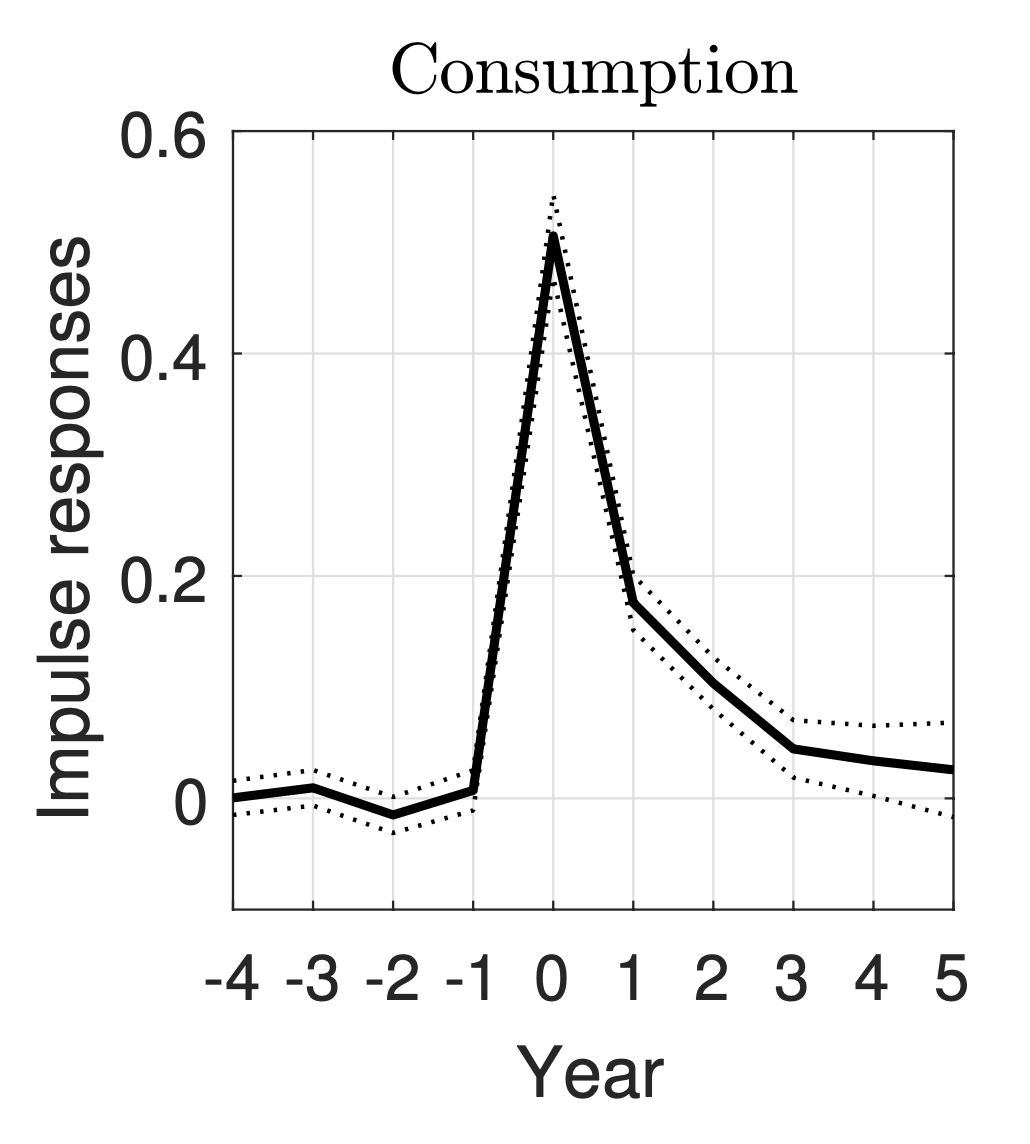
\includegraphics[scale=0.35]{figures/LotteryMPCestimate.png}}
     &  \parbox{0.4\textwidth}{
     		
            \begin{itemize}
                \item Provides estimate of first column of $\nabla_{\bm{Y}}\pmb{\mathbb{C}}$. 
                \item Need a model to extrapolate. 
%                \item Key 
            \end{itemize} Source: Fagereng, Holm, Natvik (2018) } 
%            \\
%             & 
%    $\bullet$  \\
 %    \begin{itemize}
%        \item Provides estimate of first column.
%        \item Need a model to extrapolate.
%    \end{itemize}
    \end{tabular}
\end{frame}


\begin{frame}
    \frametitle{iMPCs in the Models}
    \centering
    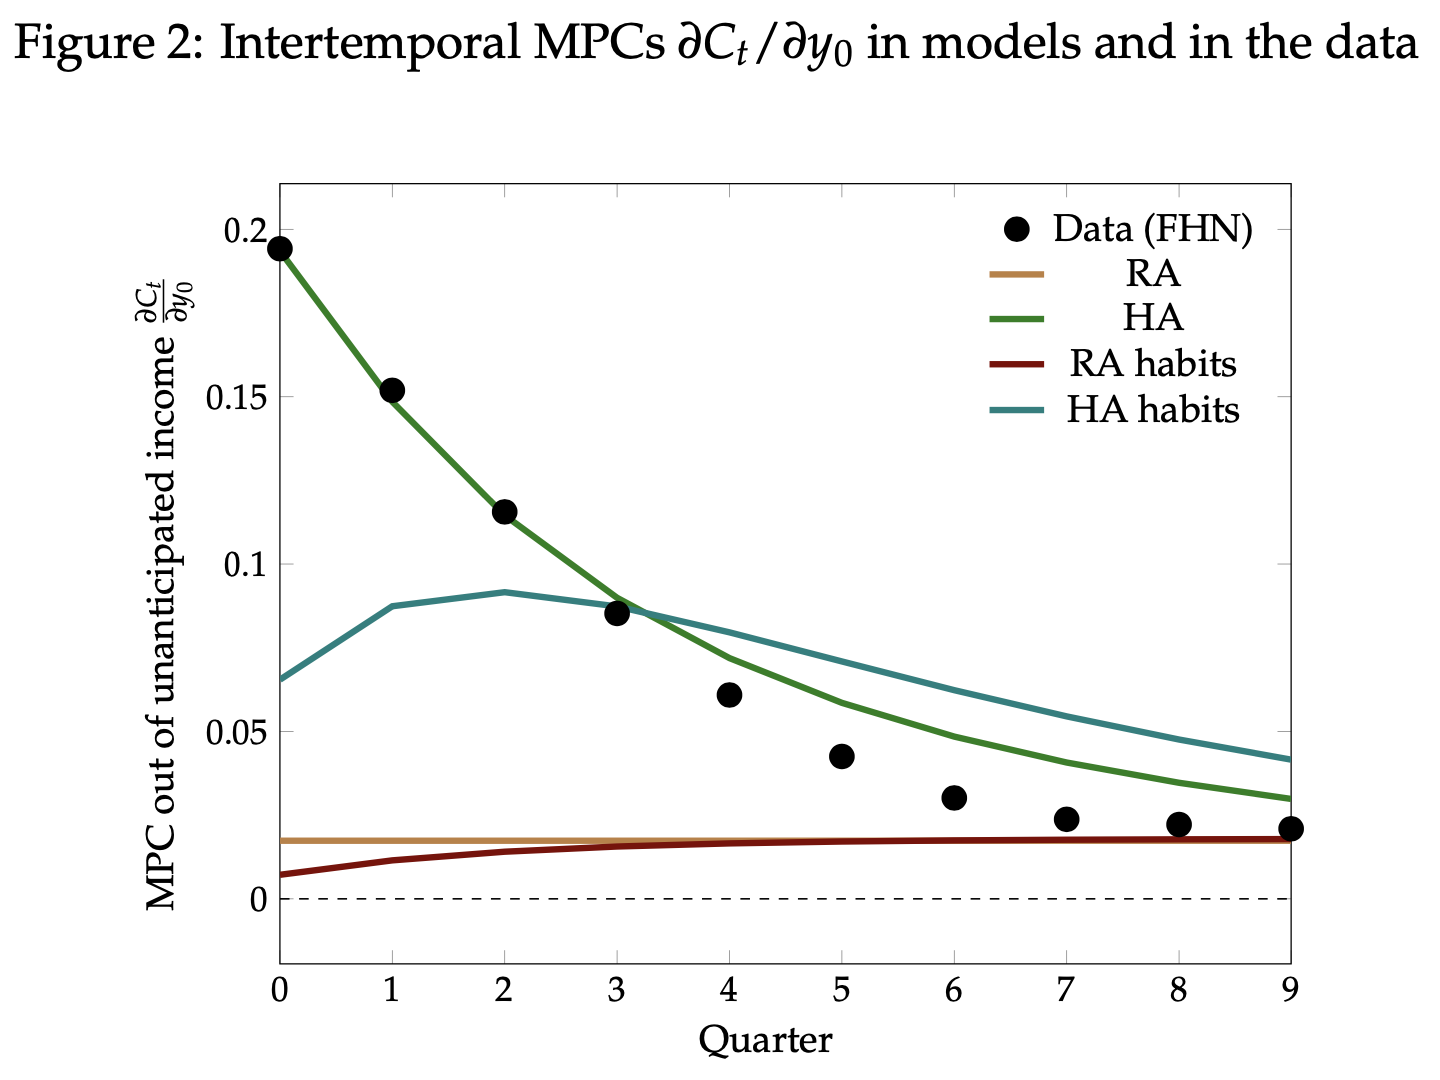
\includegraphics[scale=0.4]{figures/ARSFIG2.png}
\end{frame}

%\begin{frame}
%    \frametitle{Bonus: Durables}
%    Own figure
%\end{frame}

\begin{frame}
    \frametitle{Model Extrapolation}
    \centering
    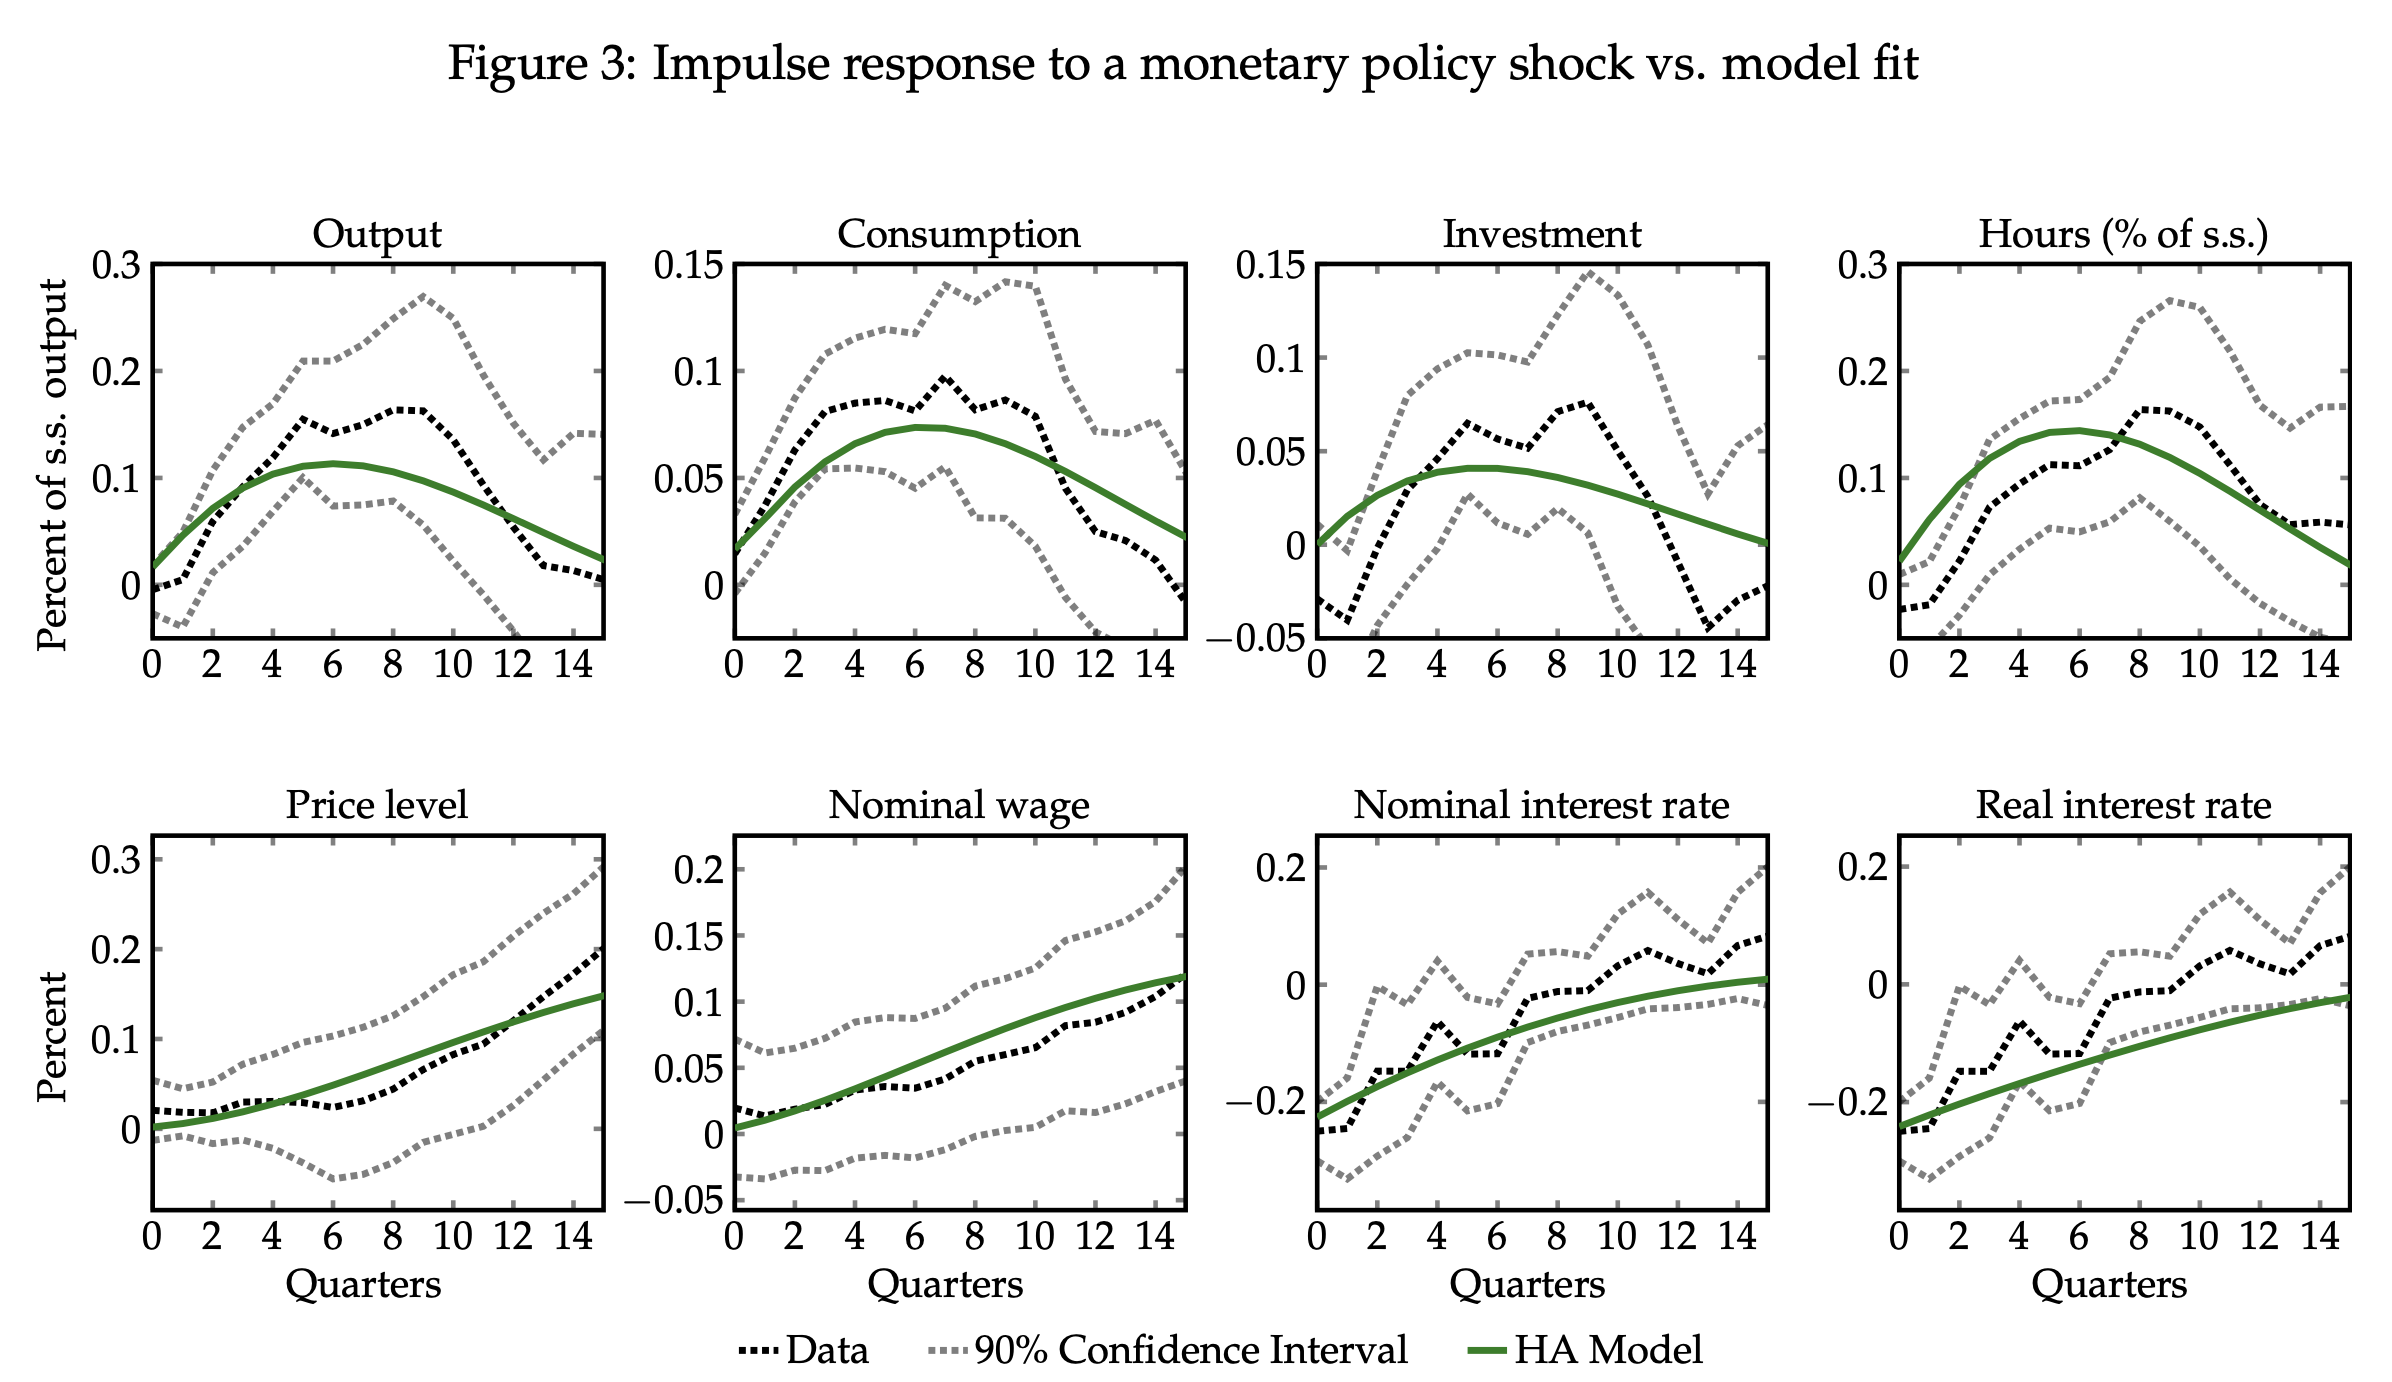
\includegraphics[scale=0.3]{figures/ARSFIG3.png}
\end{frame}


\begin{frame}
    \frametitle{Fiscal Policies: All Models}
    \centering
    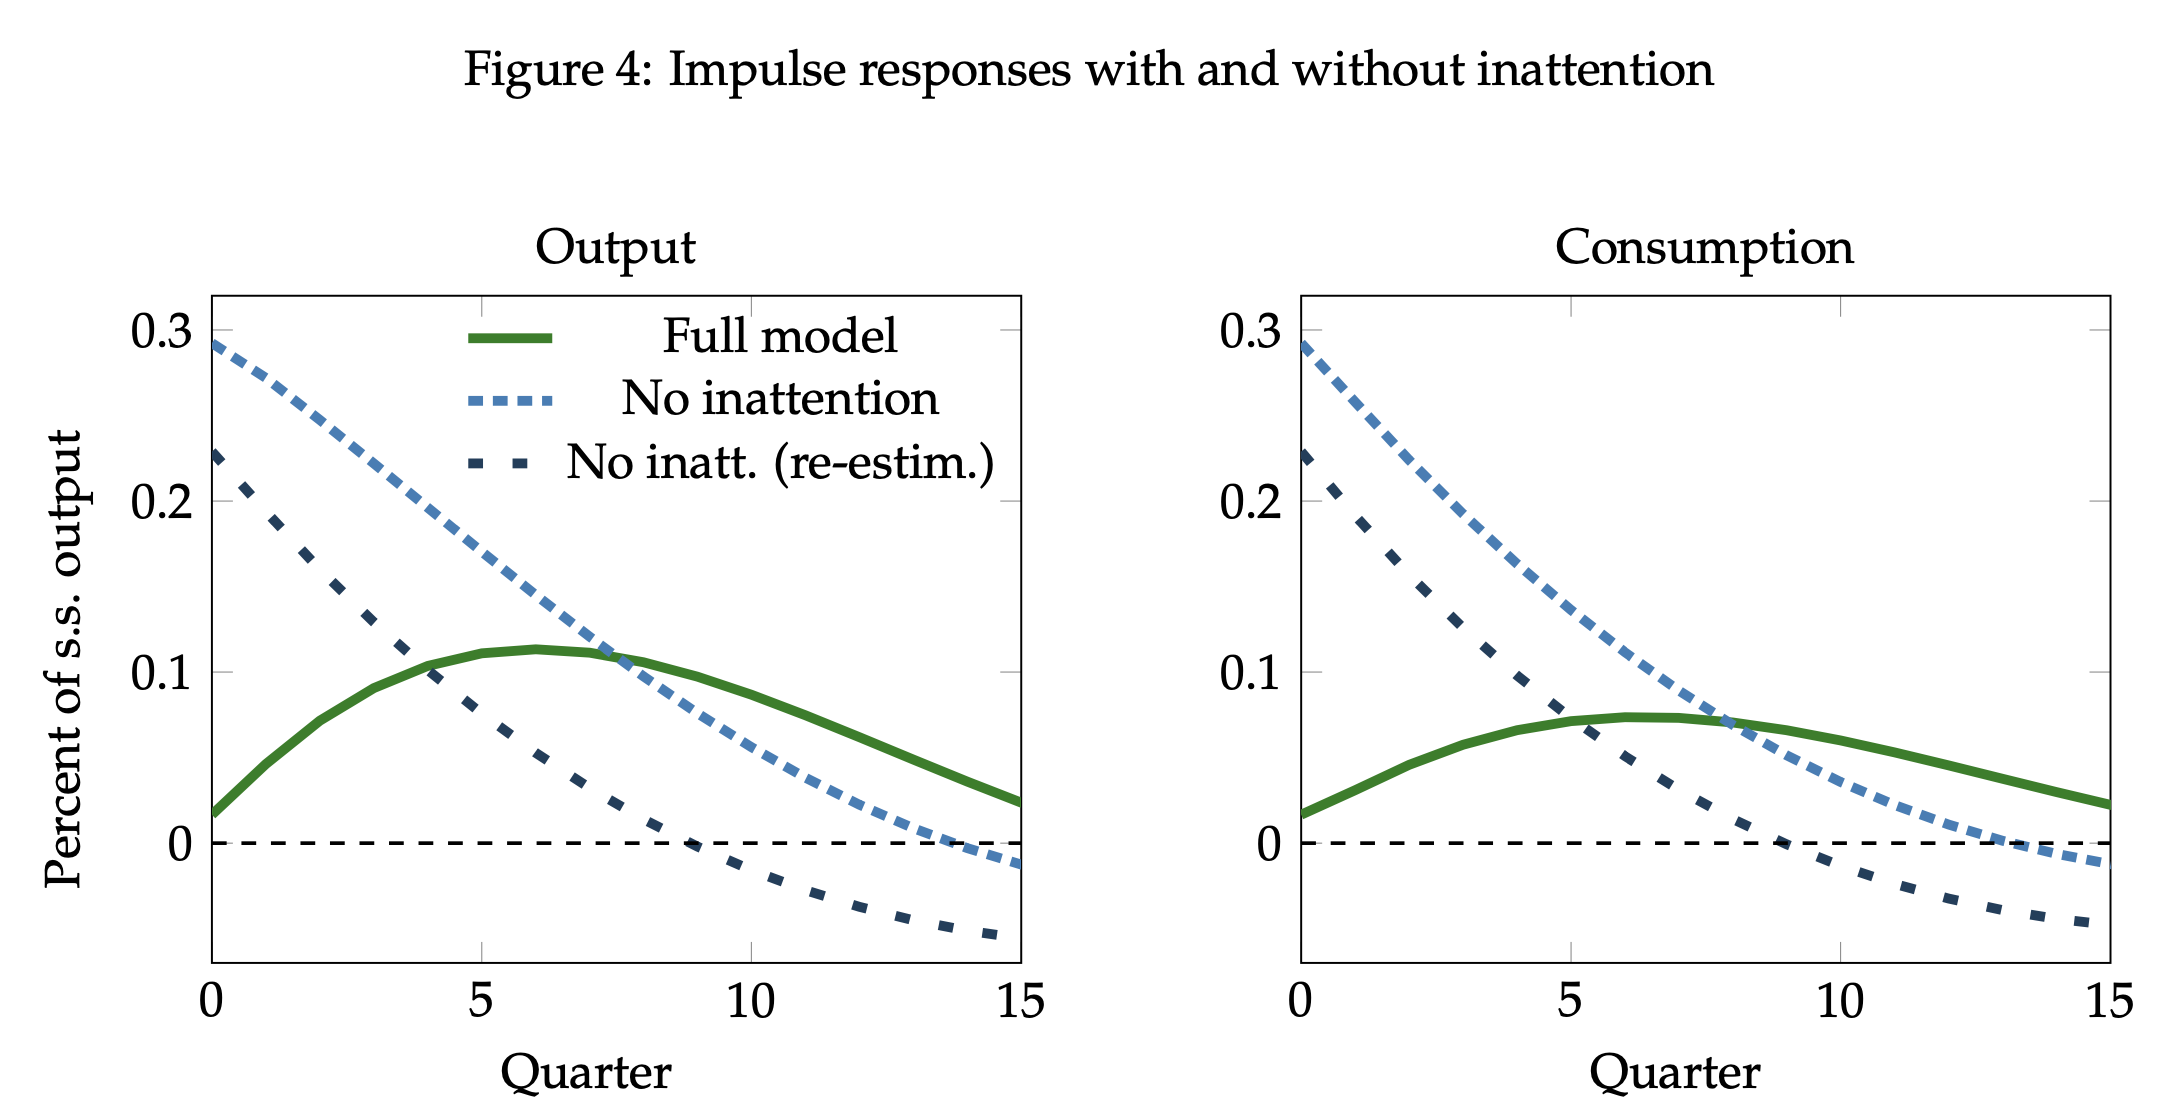
\includegraphics[scale=0.3]{figures/ARSFIG4.png}
\end{frame}

%\begin{frame}
%    \frametitle{Bonus: Regional Estimates?}
%    Own figure
%\end{frame}


\begin{frame}
    \frametitle{Quantitative Model}
    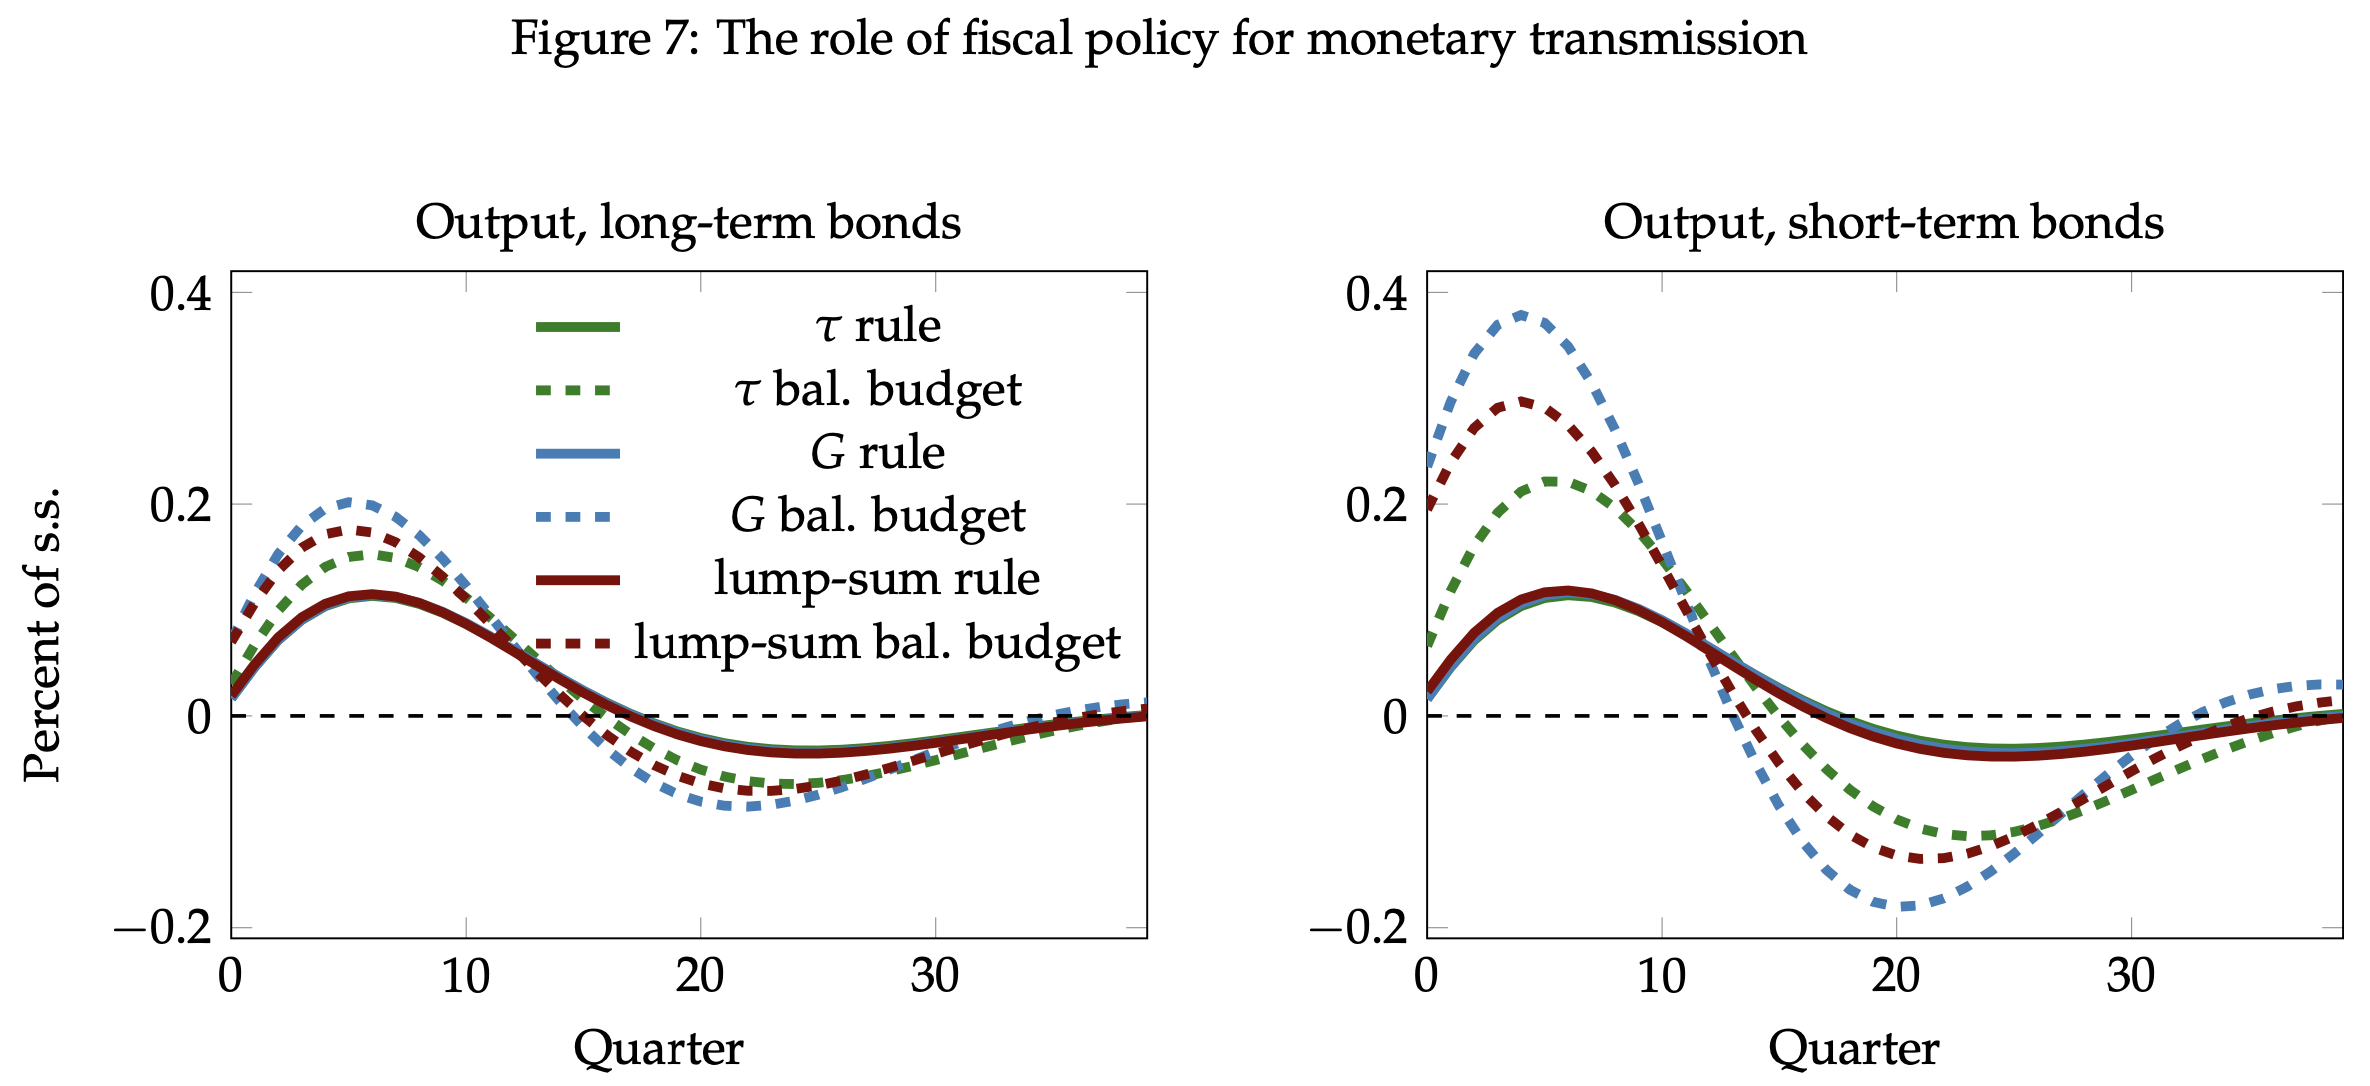
\includegraphics[scale=0.3]{figures/ARSFIG7.png}
    \begin{itemize}
    	\item What does this tell us about supply elasticities?
    \end{itemize}
\end{frame}

\begin{frame}
    \frametitle{Private Deficits}
    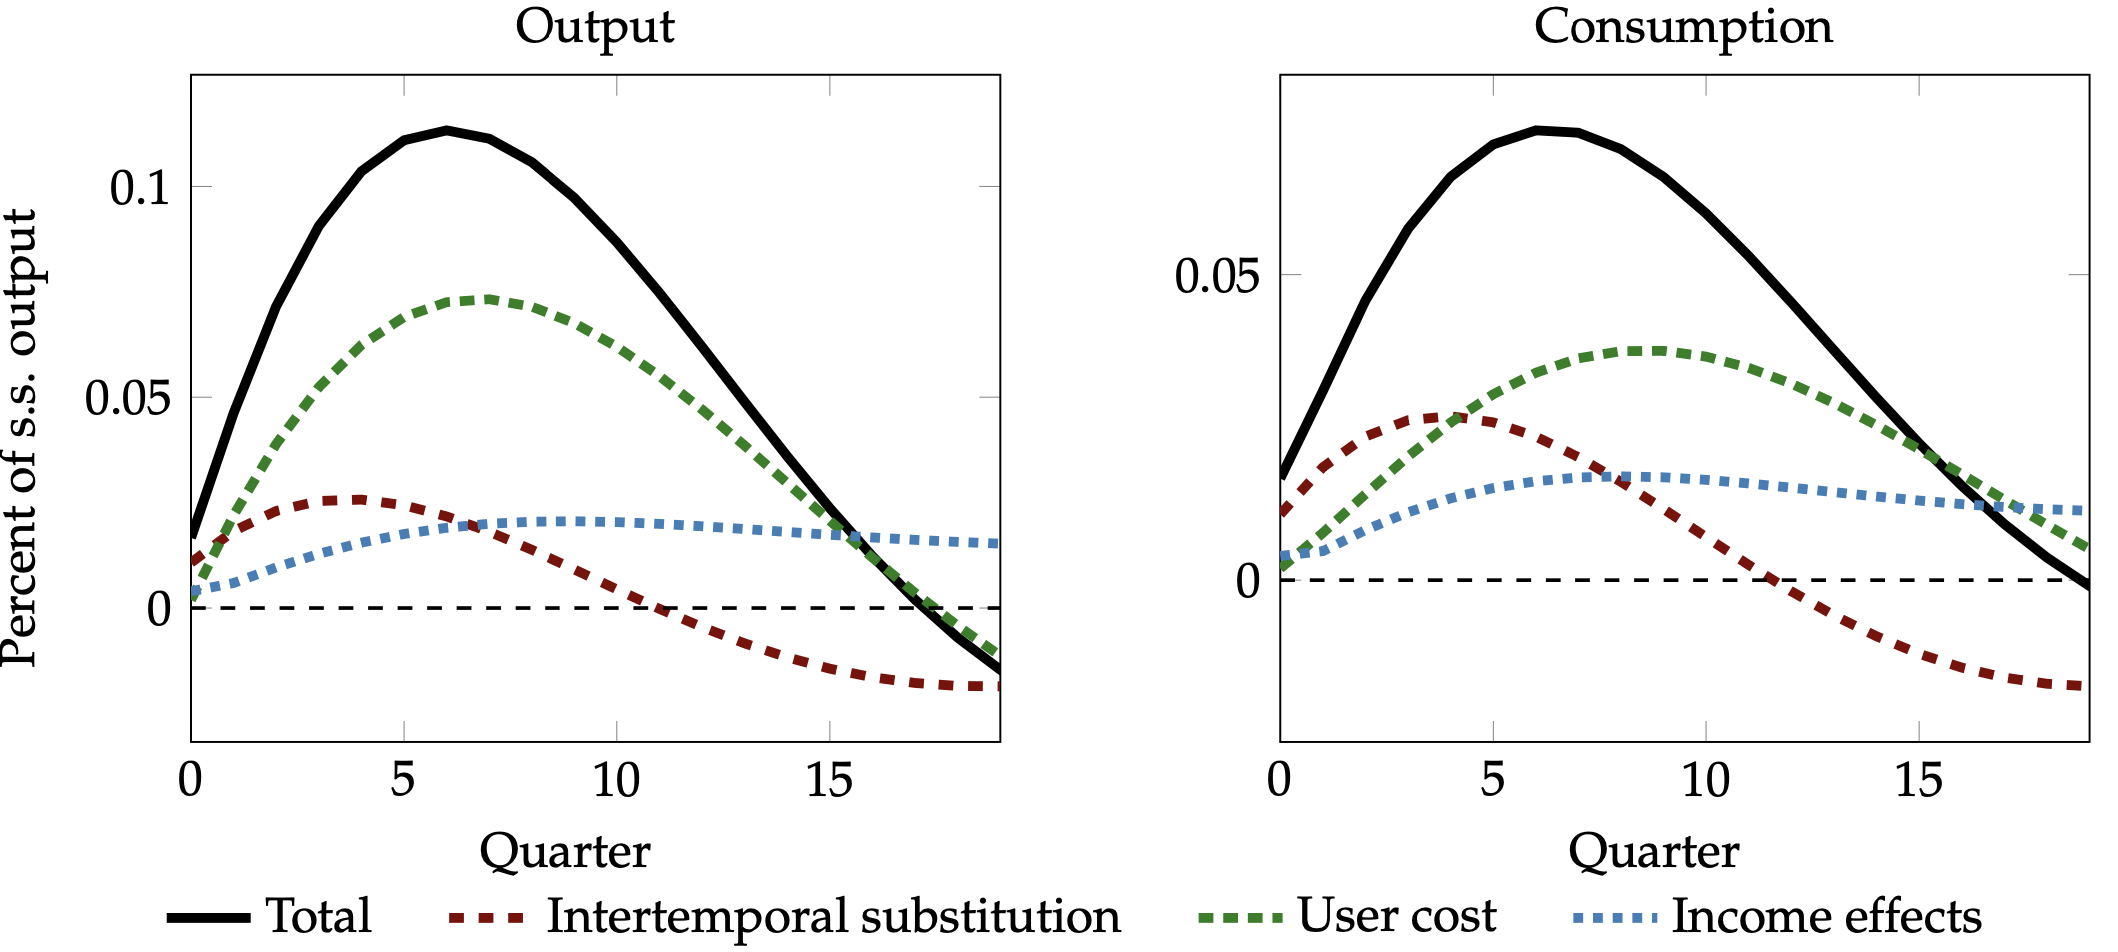
\includegraphics[scale=0.3]{figures/ARSFIG8.png}
    \begin{itemize}
    	\item Why so much amplification?
    \end{itemize}
\end{frame}


%%%%%%%%%%%%%%%%%%%%%%%%%%%%%%%%%%%%%%%%%%%%%%%%%%
\section{Auclert, Rognlie, Straub (2020)}
%%%%%%%%%%%%%%%%%%%%%%%%%%%%%%%%%%%%%%%%%%%%%%%%%%

\begin{frame}
    \frametitle{New Keynesian Model in Sequence Space}
    \begin{itemize}
        \item Consumption function:
        \begin{align*}
            C_t &= \mathbb{C}(\{Y_{t+s}-T_{t+s},r_{t+s}\}_{s=0}^{\infty}) \\
            &\equiv \mathbb{C}(\bm{Y}-\bm{T},\bm{r})
        \end{align*}
        \item NKPC:
        \begin{align*}
            \pi_t &= \mathbb{S}(\bm{Y} - \bm{Y}^*) 
        \end{align*}
        \item Interest rate rule:
        \begin{align*}
            \bm{r} &= \bm{\Phi}_Y (\bm{Y} - \bm{Y}^*) +  \bm{\Phi}_\pi \bm{\pi} + \bm{\epsilon}^r 
        \end{align*}
        \item Excess demand:
        \begin{align*}
%            \begin{pmatrix} ED_t \\ ED_{t+1} \\ \vdots \end{pmatrix}= 
            \bm{ED} &= \pmb{\mathbb{C}}(\bm{Y}-\bm{T},\bm{r}) + \bm{G} - \bm{Y} =\bm{0}
        \end{align*}
%        \item In equilibrium, $\bm{ED}=\bm{0}$.
    \end{itemize}
\end{frame}

\begin{frame}
    \frametitle{Linearize to Solve with Linear Algebra}
    \begin{itemize}
        \item Linearized Model:
        \begin{align*}
            \bm{\hat{C}} &= (\nabla_{\bm{Y}}\pmb{\mathbb{C}}) (\bm{\hat{Y}} - \bm{\hat{T}}) + (\nabla_{\bm{r}}\pmb{\mathbb{C}})\bm{\hat{r}} \\
            \bm{\hat{\pi}} &= (\nabla_{\bm{Y}}\pmb{\mathbb{S}})(\bm{\hat{Y}} - \bm{\hat{Y}}^*)  \\
            \bm{\hat{r}} &= \bm{\Phi}_Y (\bm{\hat{Y}} - \bm{\hat{Y}}^*) +  \bm{\Phi}_\pi \bm{\hat{\pi}} + \bm{\epsilon}^r 
        \end{align*}
        \item Equilibrium:
         \begin{align*}
             \bm{\hat{Y}} &=  [ \bm{\Phi}_Y  +  \bm{\Phi}_\pi (\nabla_{\bm{Y}}\pmb{\mathbb{S}}) ]^{-1} \{[ \bm{\Phi}_Y  +  \bm{\Phi}_\pi (\nabla_{\bm{Y}}\pmb{\mathbb{S}}) ]^{-1} - [I - \nabla_{\bm{Y}}\pmb{\mathbb{C}}]^{-1}(\nabla_{\bm{r}}\pmb{\mathbb{C}})  \}^{-1}  \times\\ 
             &\times[I - \nabla_{\bm{Y}}\pmb{\mathbb{C}}]^{-1} [\bm{\hat{G}} - (\nabla_{\bm{Y}}\pmb{\mathbb{C}})\bm{\hat{T}} + (\nabla_{\bm{r}}\pmb{\mathbb{C}})\bm{\epsilon}^r ]  
         \end{align*}
         \item Kaplan, Moll, and Violante (2018):
         \begin{itemize}
         	\item Small direct effect $\nabla_{\bm{r}}\pmb{\mathbb{C}}$
         	\item Large indirect effect $[I - \nabla_{\bm{Y}}\pmb{\mathbb{C}}]^{-1}$
         	\item Product roughly constant $[I - \nabla_{\bm{Y}}\pmb{\mathbb{C}}]^{-1}(\nabla_{\bm{r}}\pmb{\mathbb{C}})$
         \end{itemize}
         \item[$\Rightarrow$] Should we care about the decomposition?
    \end{itemize}
\end{frame}


\begin{frame}
    \frametitle{Add Investment}
    \begin{itemize}
        \item Yes:
        \begin{align*}
             \bm{\hat{Y}} &=  [ \bm{\Phi}_Y  +  \bm{\Phi}_\pi (\nabla_{\bm{Y}}\pmb{\mathbb{S}}) ]^{-1} \times \\
             &\times \{[ \bm{\Phi}_Y  +  \bm{\Phi}_\pi (\nabla_{\bm{Y}}\pmb{\mathbb{S}}) ]^{-1} - [I - \nabla_{\bm{Y}}\pmb{\mathbb{C}} - \nabla_{\bm{Y}}\pmb{\mathbb{I}} ]^{-1}(\nabla_{\bm{r}}\pmb{\mathbb{C}} + \nabla_{\bm{r}}\pmb{\mathbb{I}})  \}^{-1}  \times\\ 
             &\times[I - \nabla_{\bm{Y}}\pmb{\mathbb{C}}- \nabla_{\bm{Y}}\pmb{\mathbb{I}}]^{-1} [\bm{\hat{G}} - (\nabla_{\bm{Y}}\pmb{\mathbb{C}})\bm{\hat{T}} + (\nabla_{\bm{r}}\pmb{\mathbb{C}}+\nabla_{\bm{r}}\pmb{\mathbb{I}})\bm{\epsilon}^r ]  
         \end{align*}
        \item Key challenge: How to set up model to match 
        \begin{itemize}
        	\item Immediate consumption response to higher income (``jump'').
        	\item Delayed consumption, investment, output response to lower real interest rate (``hump'').
        \end{itemize}
    \end{itemize}
\end{frame}


\begin{frame}
    \frametitle{The Challenge}
    \begin{center}
    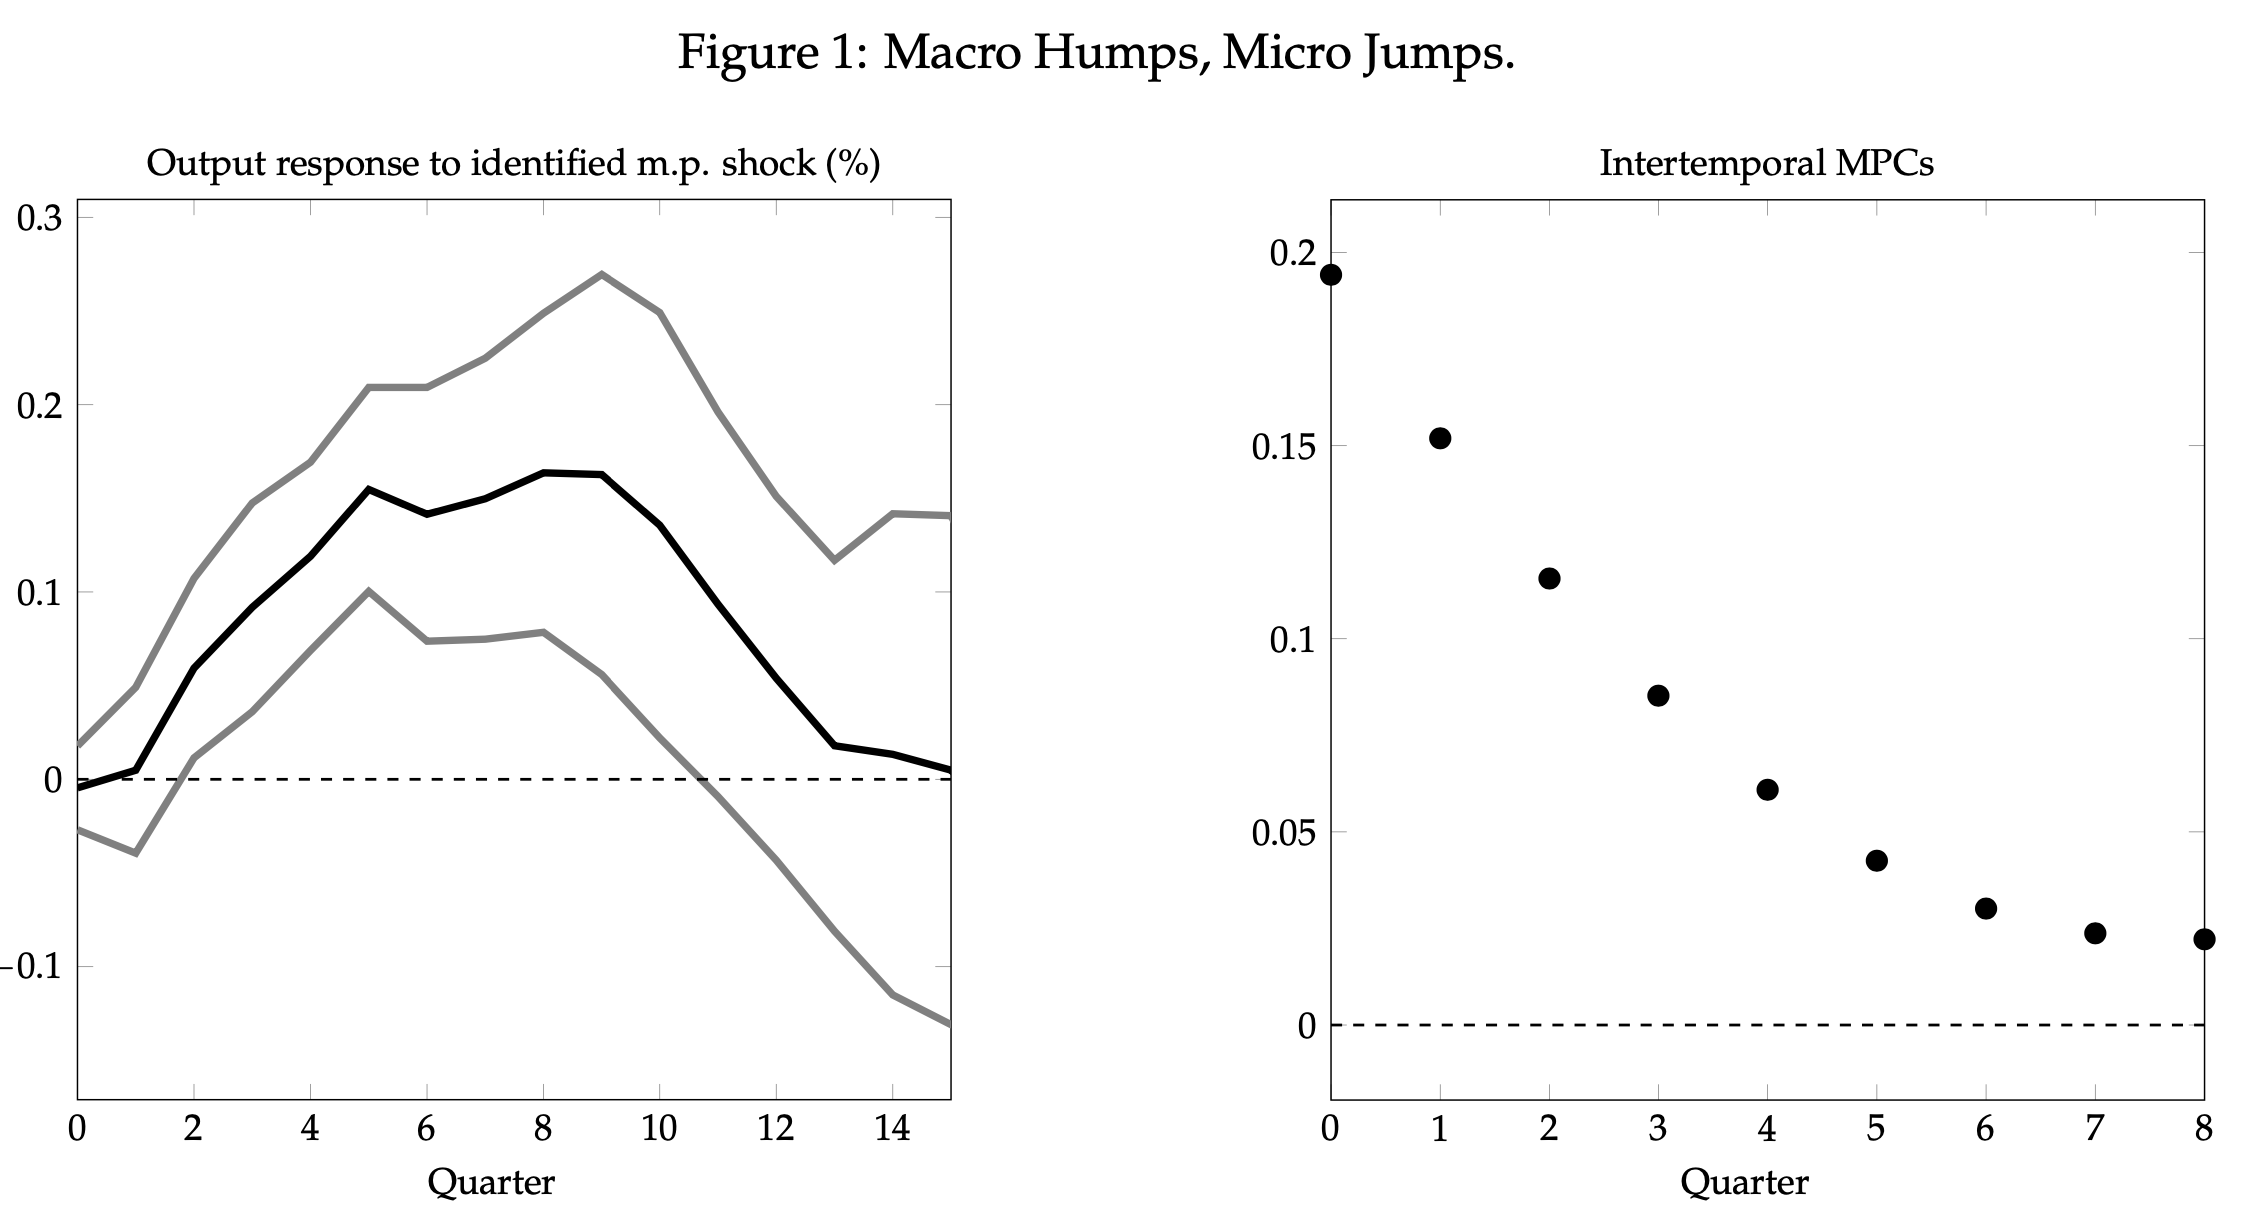
\includegraphics[scale=0.3]{figures/ARSFIG1.png}
    \end{center}
\end{frame}

\begin{frame}
    \frametitle{Model}
    \begin{itemize}
        \item Household problem:
        \begin{align*}
        	V_t(l,s) = &\max_{c,l'}u(c)+\beta\E[V_{t+1}(l',s')|s] \\
        	&c'+l' \le (1+r_t)l + y_t e(s) \\
        	& l'\ge 0
        \end{align*}
        \item Standard sequence space result:
        \begin{align*}
        	C_t = \mathcal{C}(\{y_s,r_s\}_{s\ge 0}), \;t\ge 0
        \end{align*}
    \end{itemize}
\end{frame}

\begin{frame}
    \frametitle{Matching Micro Data}
    \begin{center}
    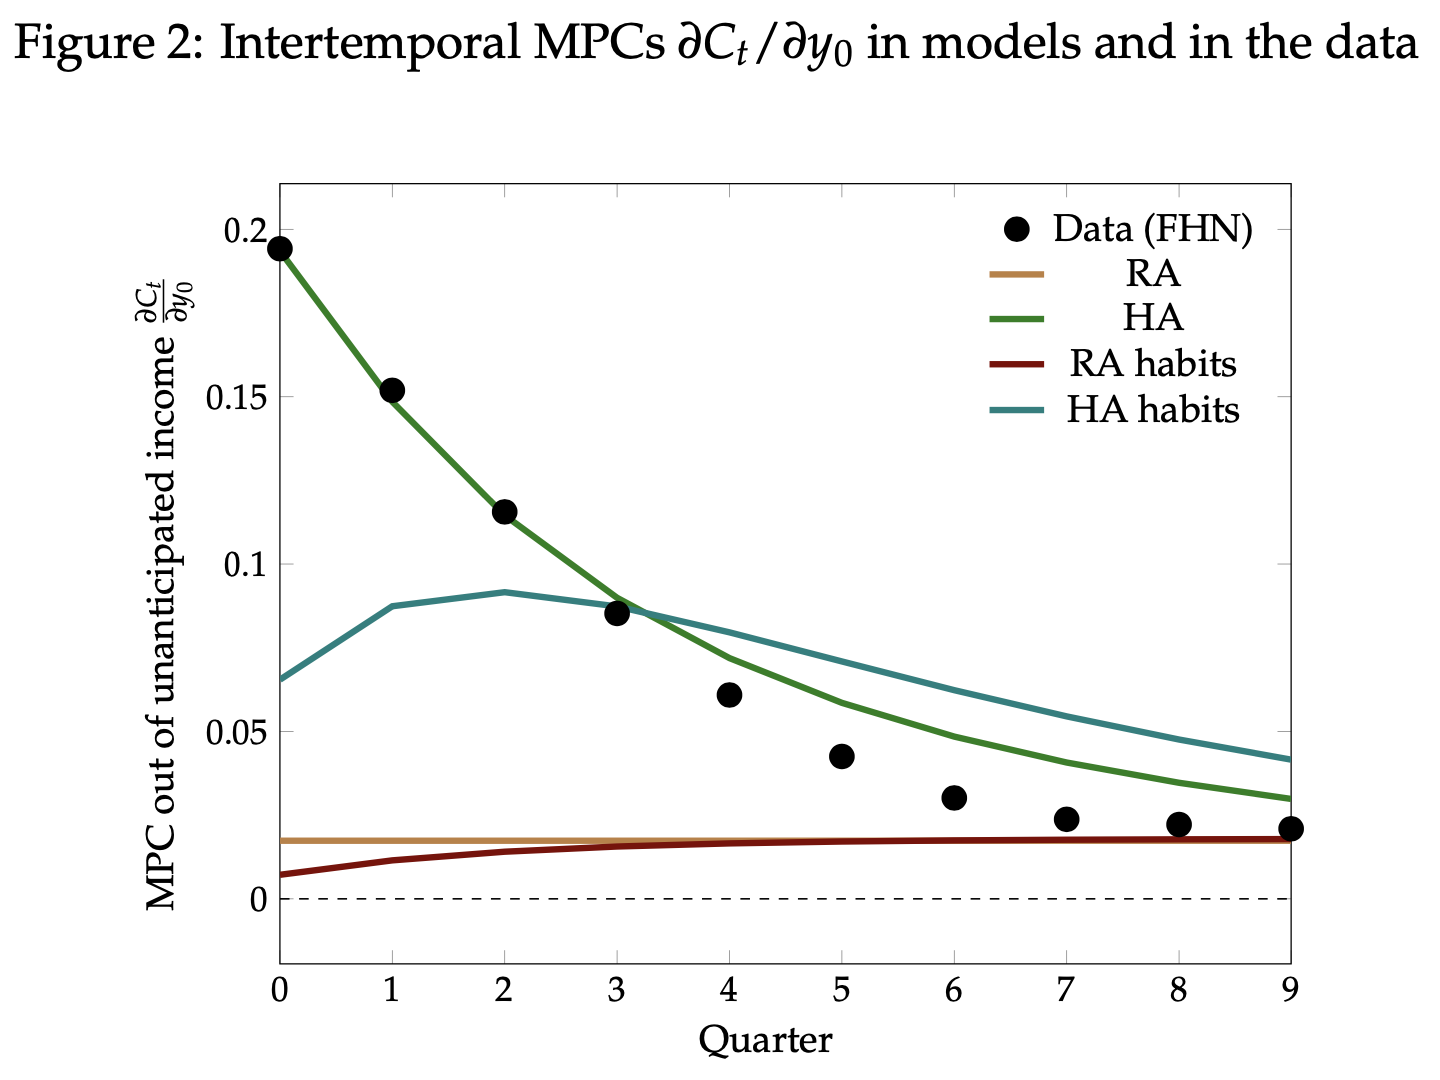
\includegraphics[scale=0.4]{figures/ARSFIG2.png}
    \end{center}
    \begin{itemize}
    	\item Why does habit model have difficulty?
    \end{itemize}
\end{frame}

\begin{frame}
    \frametitle{Inattention}
    \begin{itemize}
        \item Households know current micro state $e(s)$.
        \item Households update info about aggregate shocks with iid probability $1-\theta$ each period.
        \item Households know current $r_t,Y_t$ but forecast $r_{t+s},Y_{t+s}$ using info from $t-k$. 
        \item[$\Rightarrow$] Households always on budget constraint.
        \item Optimize subject to information from $k$ periods ago:
        \begin{align*}
        	V_t(l,s,k) = &\max_{c,l'}u(c)+\beta\E_{t-k}[\theta V_{t+1}(l',s',k+1) + (1-\theta) V_{t+1}(l',s',0)|s] 
        \end{align*}
    \end{itemize}
\end{frame}

\begin{frame}
    \frametitle{Estimation}
    \begin{itemize}
        \item Two-step procedure.
        \item Calibrate household problem to micro data, so only need to compute household sequence space Jacobians once.
        \item Estimate information and macro parameters to match estimated IRF to monetary policy shocks.
        \item Sticky info micro Jacobian at $t$ to shock at time $s$:
        \begin{align*}
        	\mathcal{J}_{t,s}^{o,i} = \begin{cases}
        		\theta\mathcal{J}_{t-1,s-1}^{o,i} + (1-\theta)\mathcal{J}_{t,s}^{o,i,FI} & t>0, s>0 \\
        		\mathcal{J}_{t,s}^{o,i,FI} & s=0 \\
        		(1-\theta)\mathcal{J}_{t,s}^{o,i,FI} & t=0, s>0
        	\end{cases}
        \end{align*}
    \end{itemize}
\end{frame}




\begin{frame}
    \frametitle{Calibration}
    \begin{center}
    	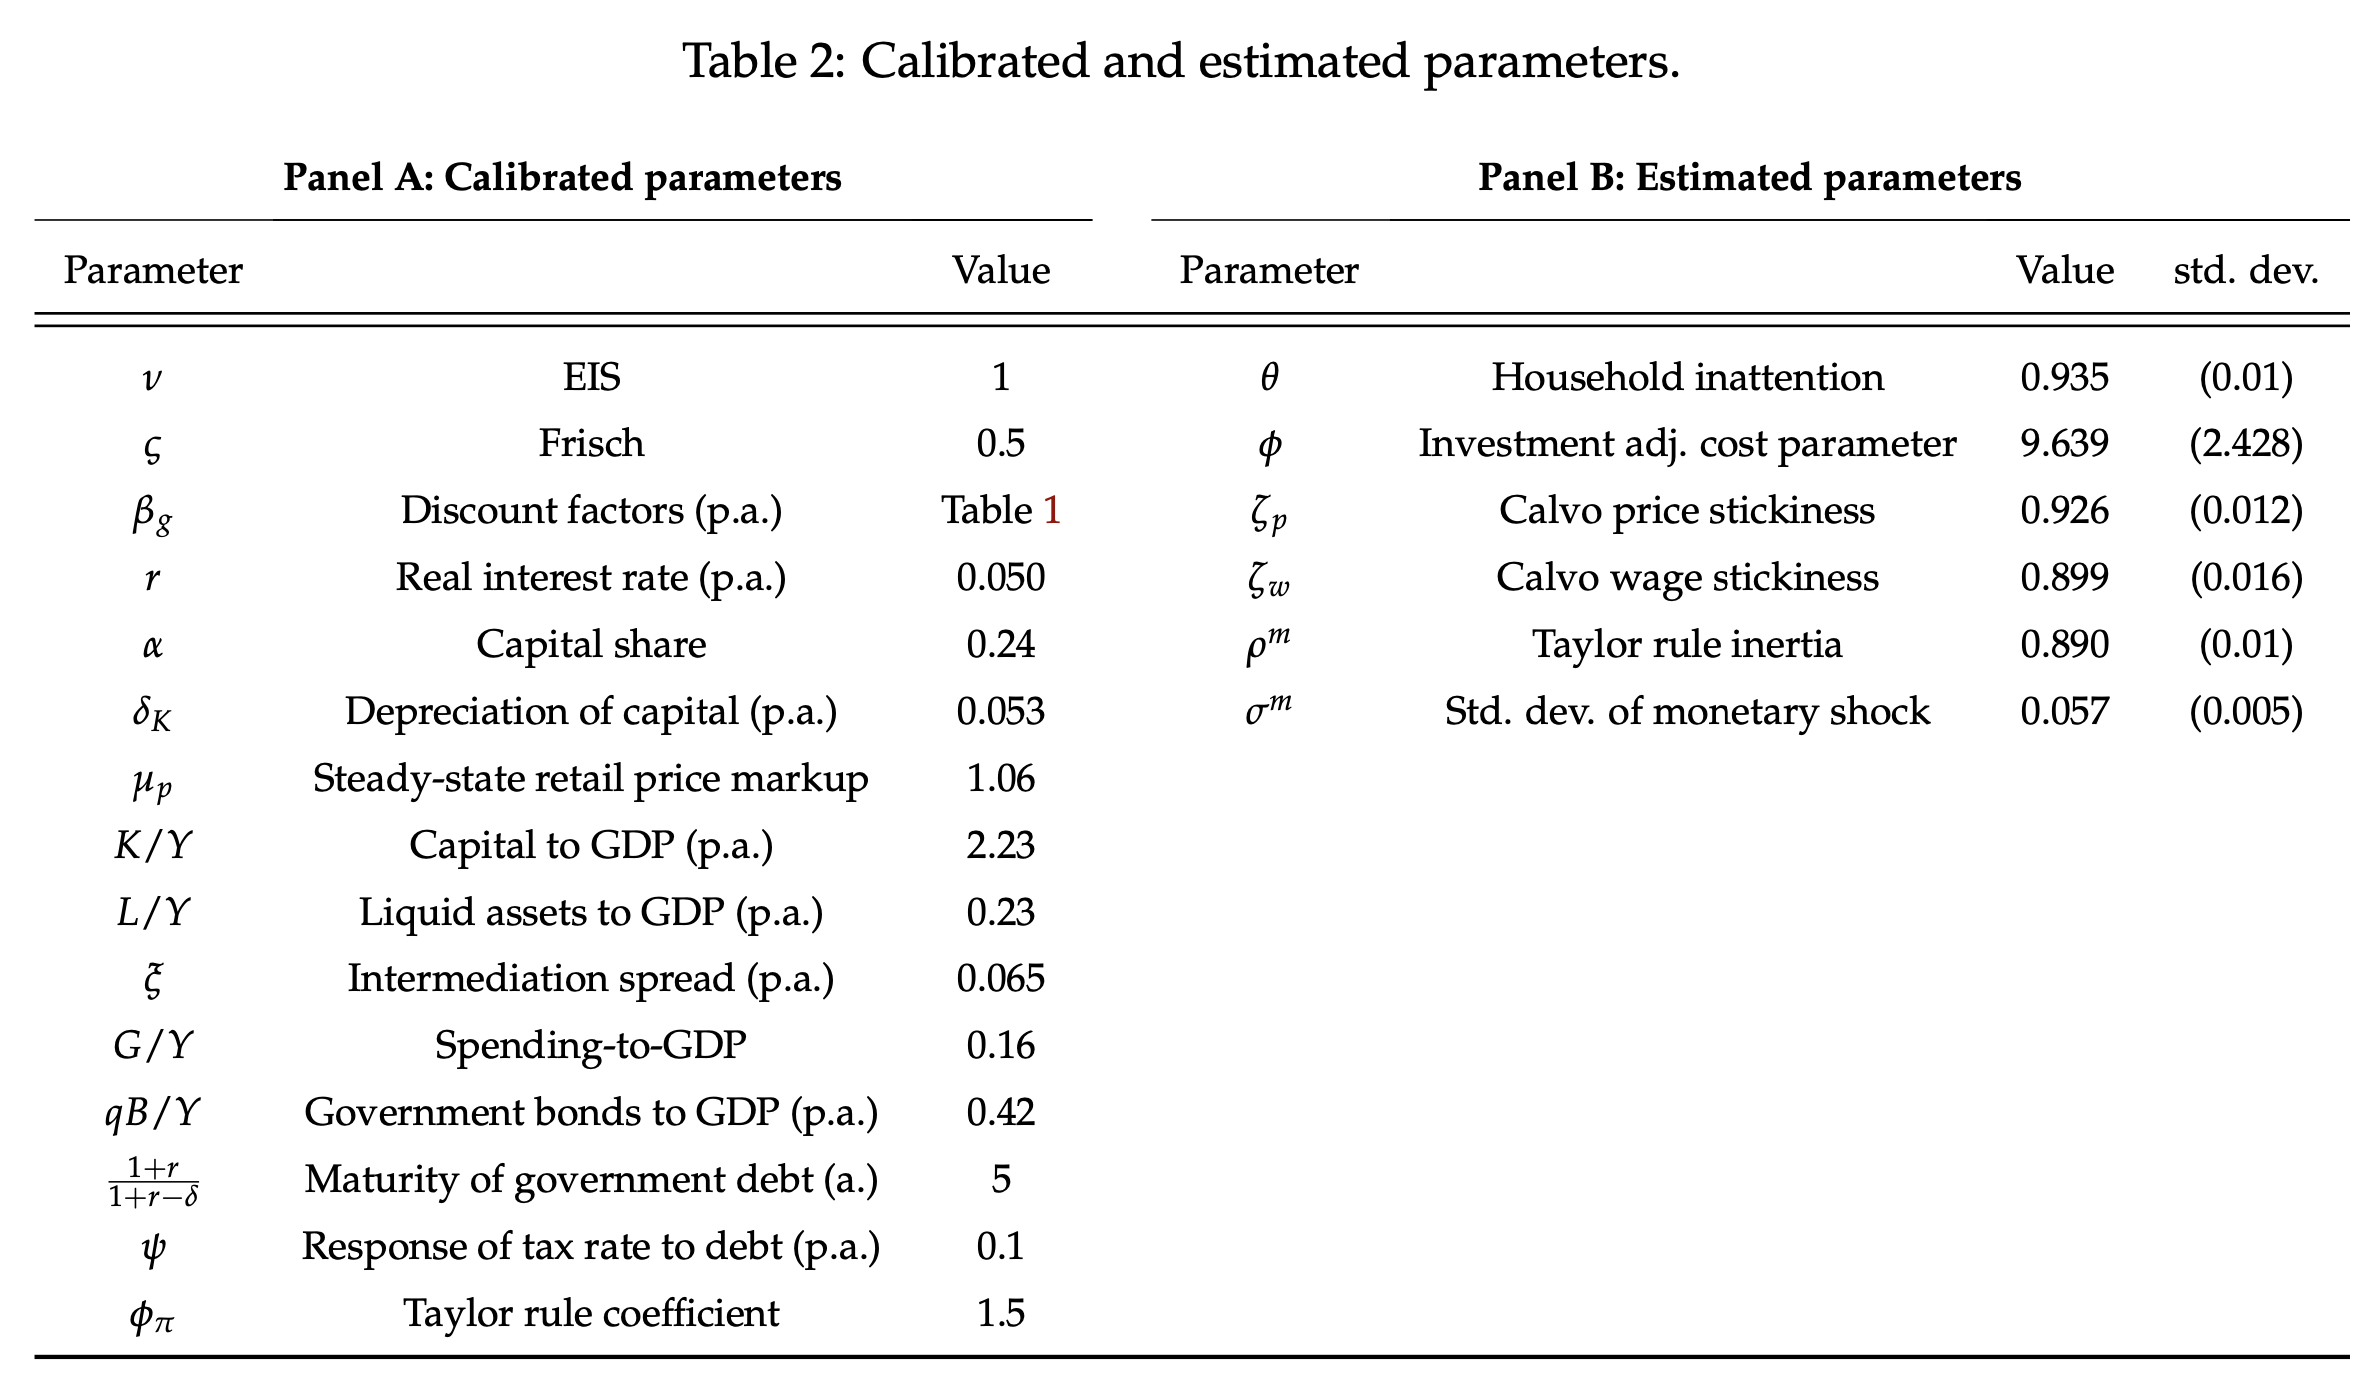
\includegraphics[scale=0.25]{figures/ARSTAB2.png}	
    \end{center}
\end{frame}


\begin{frame}
    \frametitle{Matching the Humps}
    \begin{center}
    	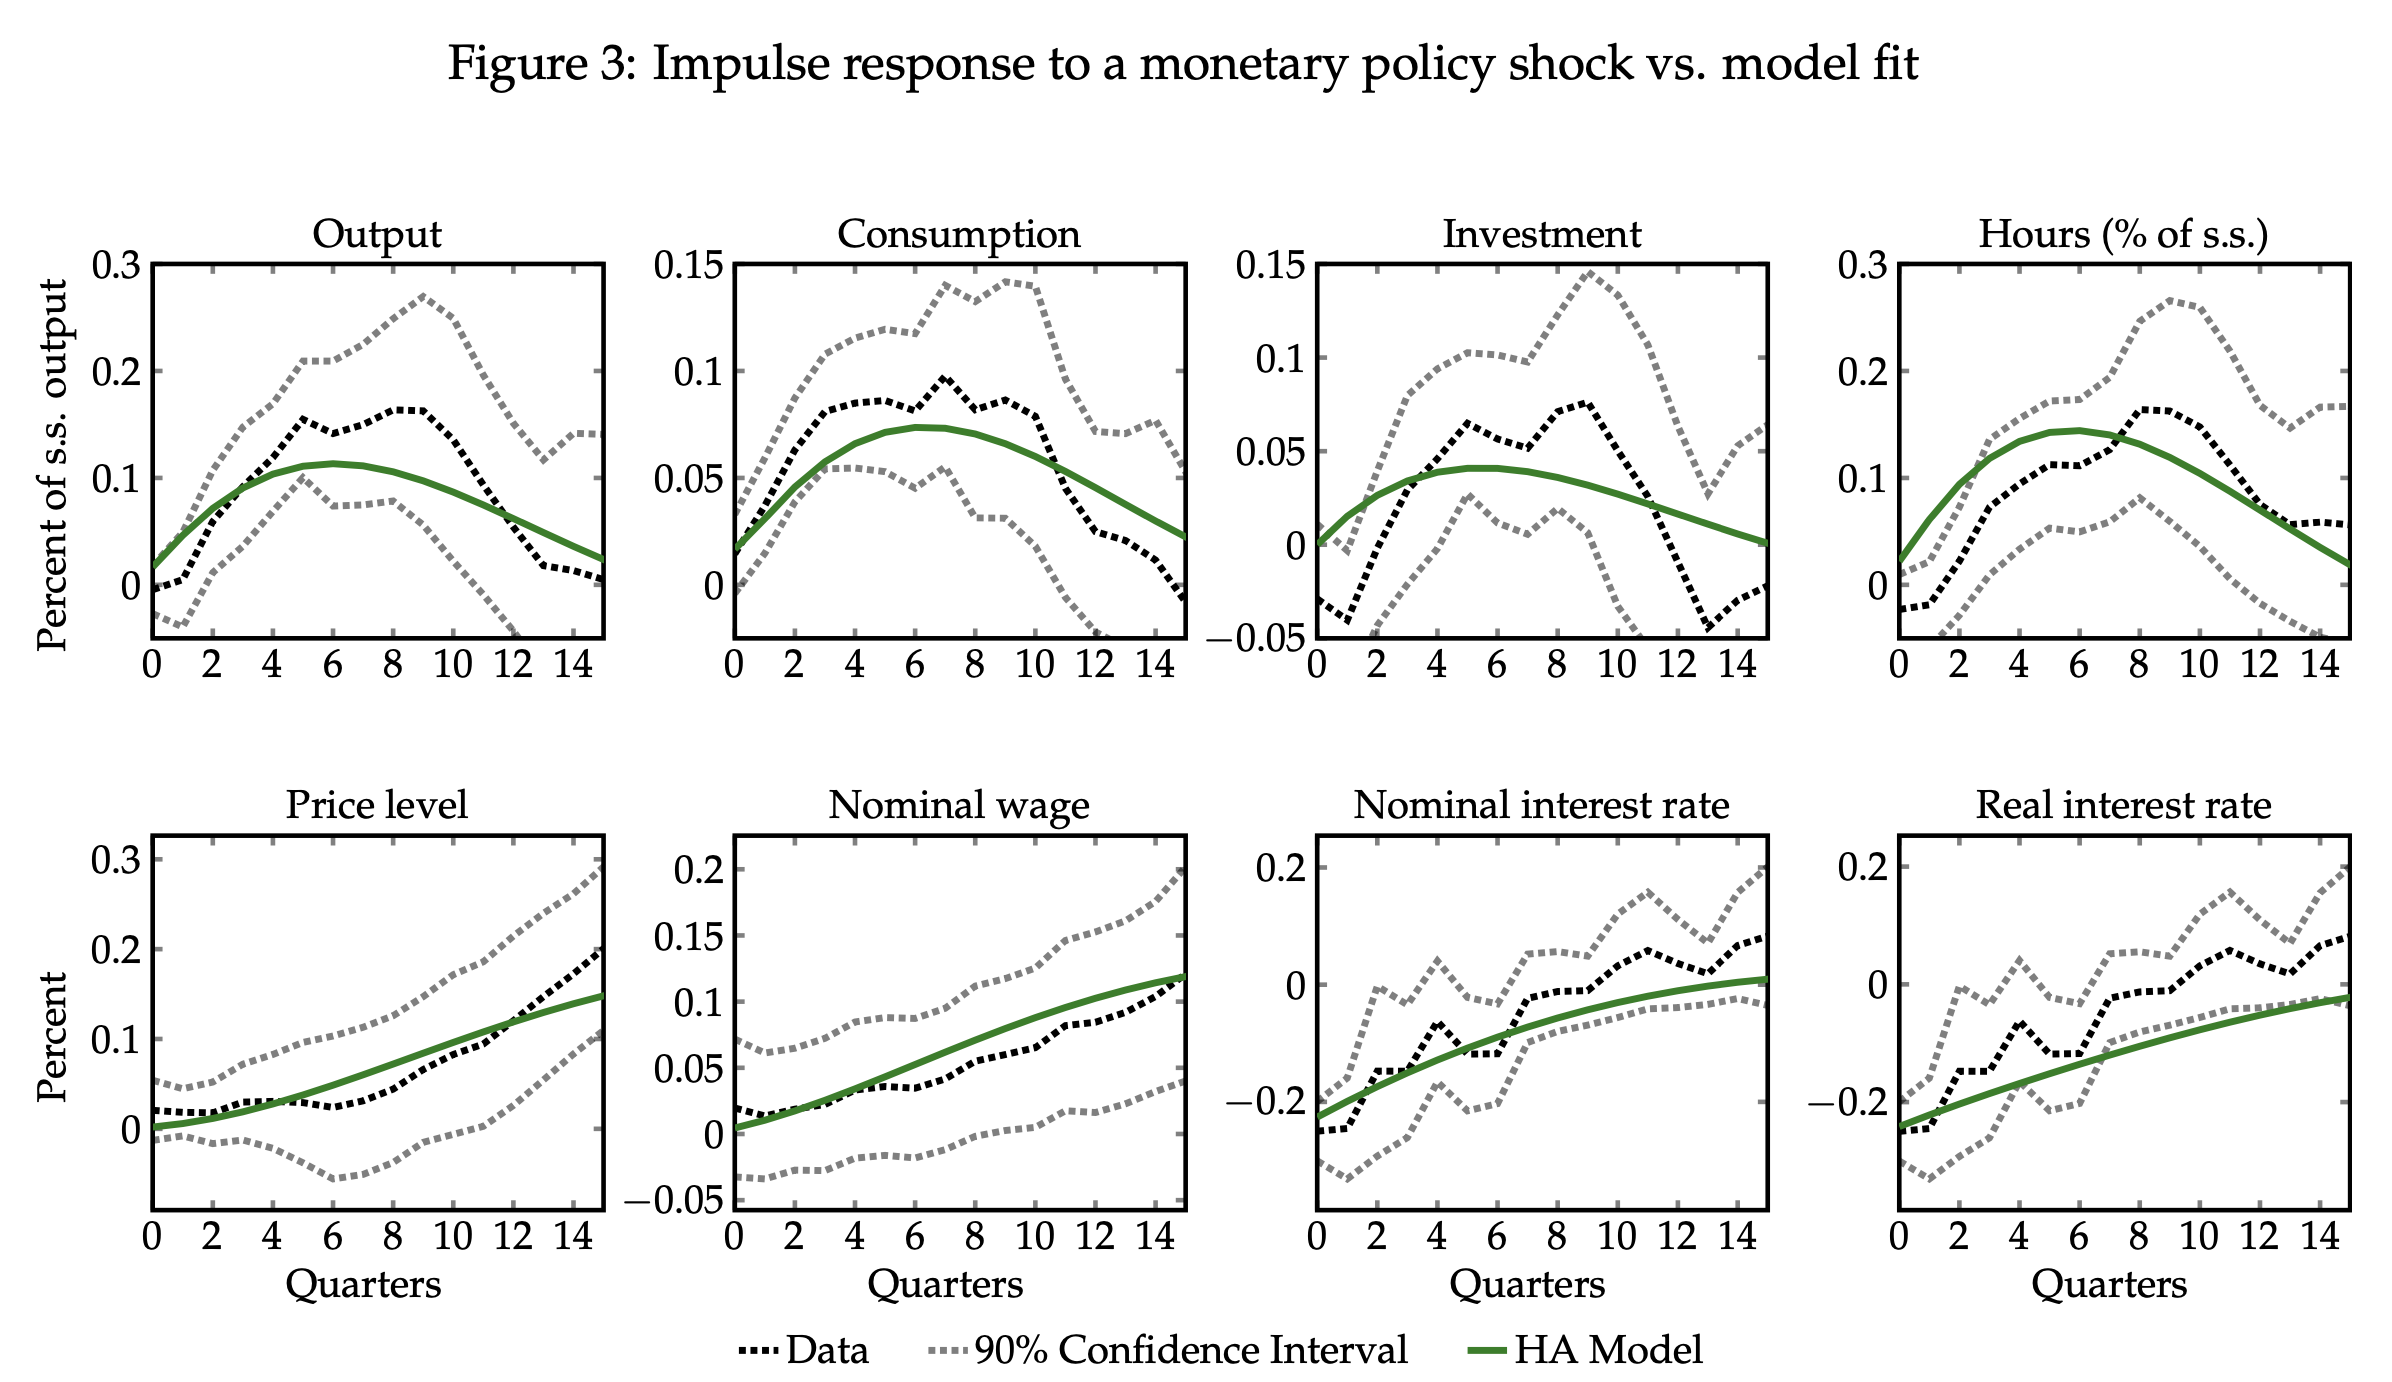
\includegraphics[scale=0.25]{figures/ARSFIG3.png}	
    \end{center}
\end{frame}

\begin{frame}
    \frametitle{Role of Inattention}
    \begin{center}
    	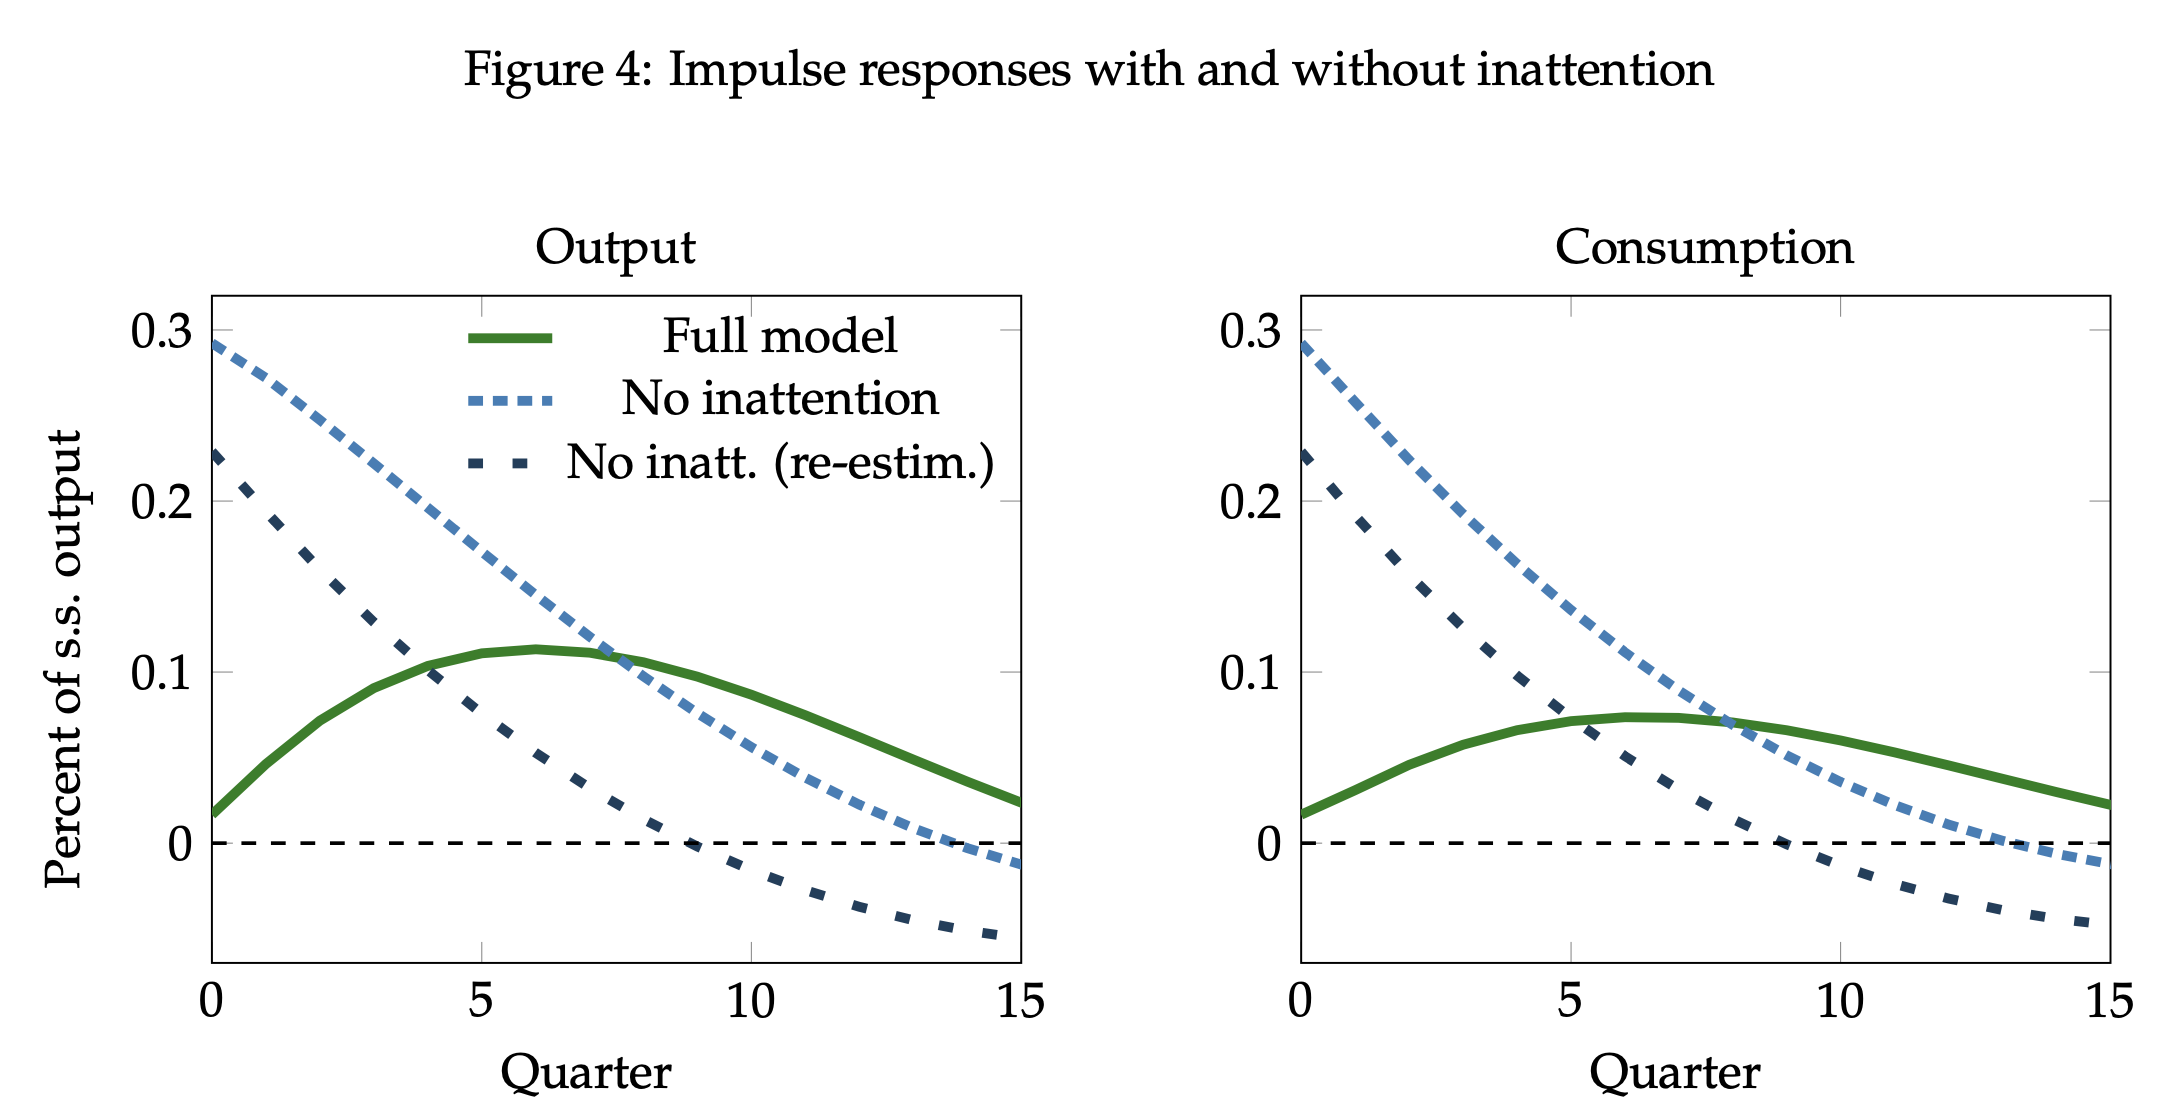
\includegraphics[scale=0.3]{figures/ARSFIG4.png}	
    \end{center}
\end{frame}


\begin{frame}
    \frametitle{Importance of Investment}
    \begin{center}
    	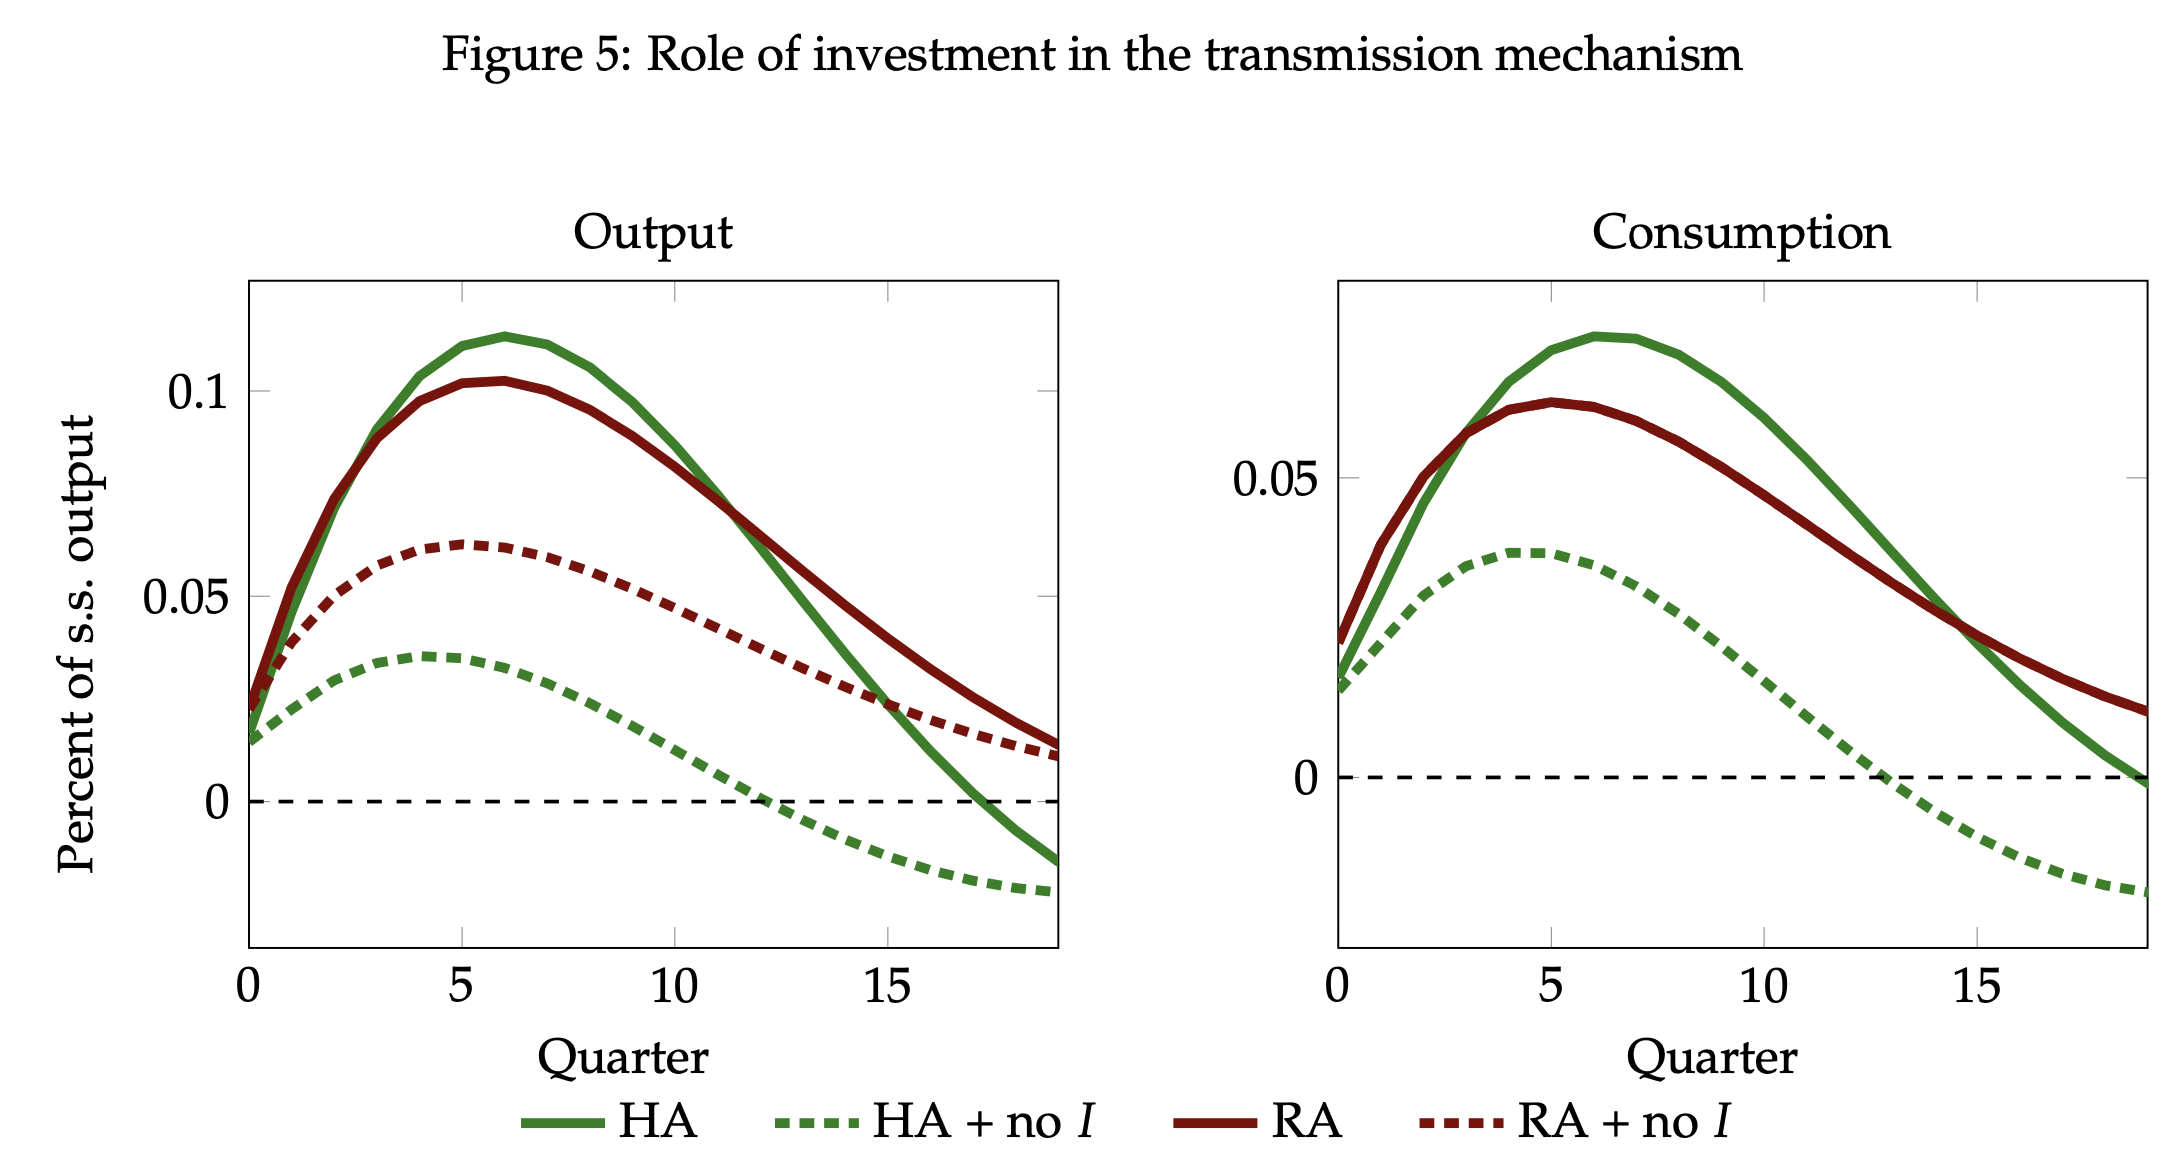
\includegraphics[scale=0.3]{figures/ARSFIG5.png}	
    \end{center}
\end{frame}

\begin{frame}
    \frametitle{Direct vs Indirect Effects}
    \begin{center}
    	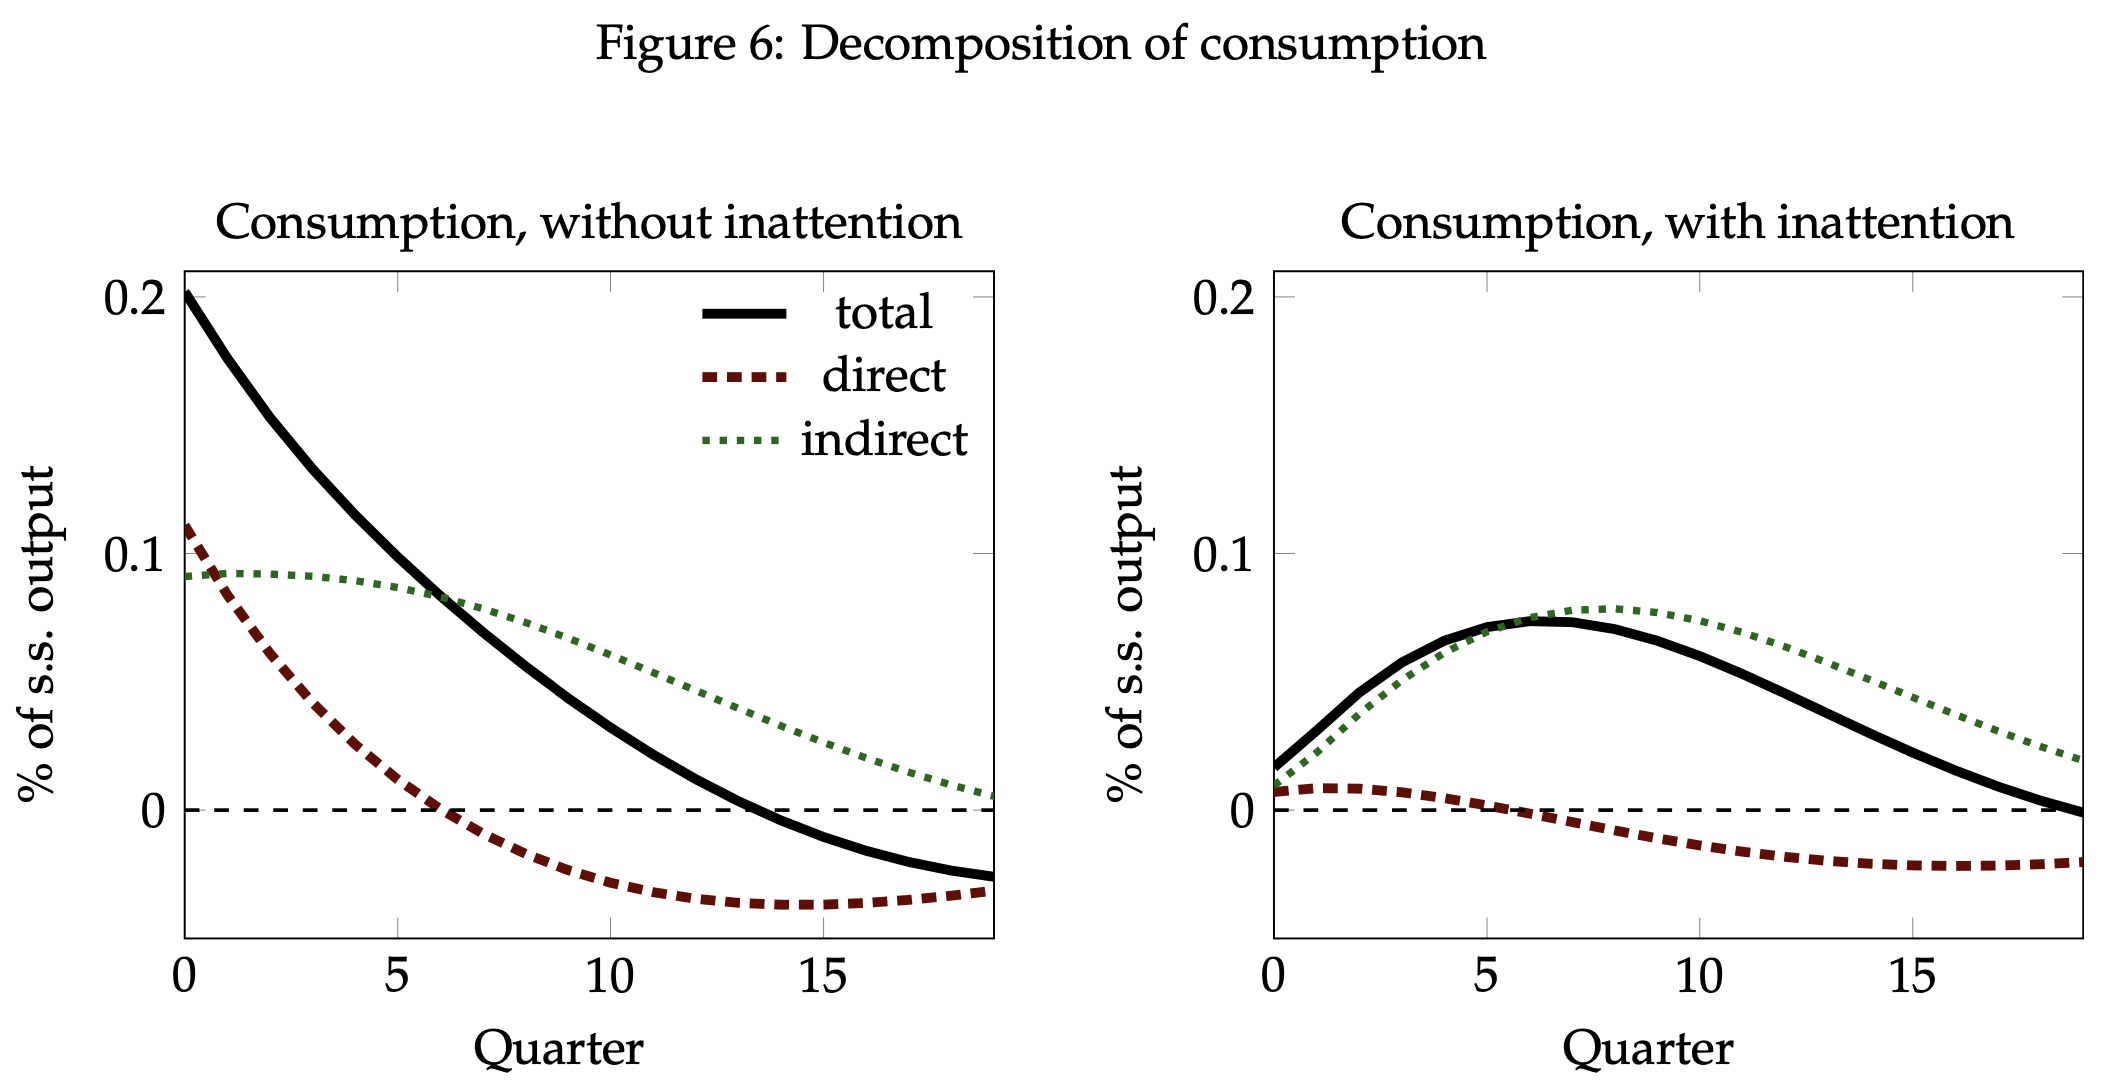
\includegraphics[scale=0.3]{figures/ARSFIG6.png}	
    \end{center}
\end{frame}

\begin{frame}
    \frametitle{Aside: Role of Fiscal Policy}
    \begin{center}
    	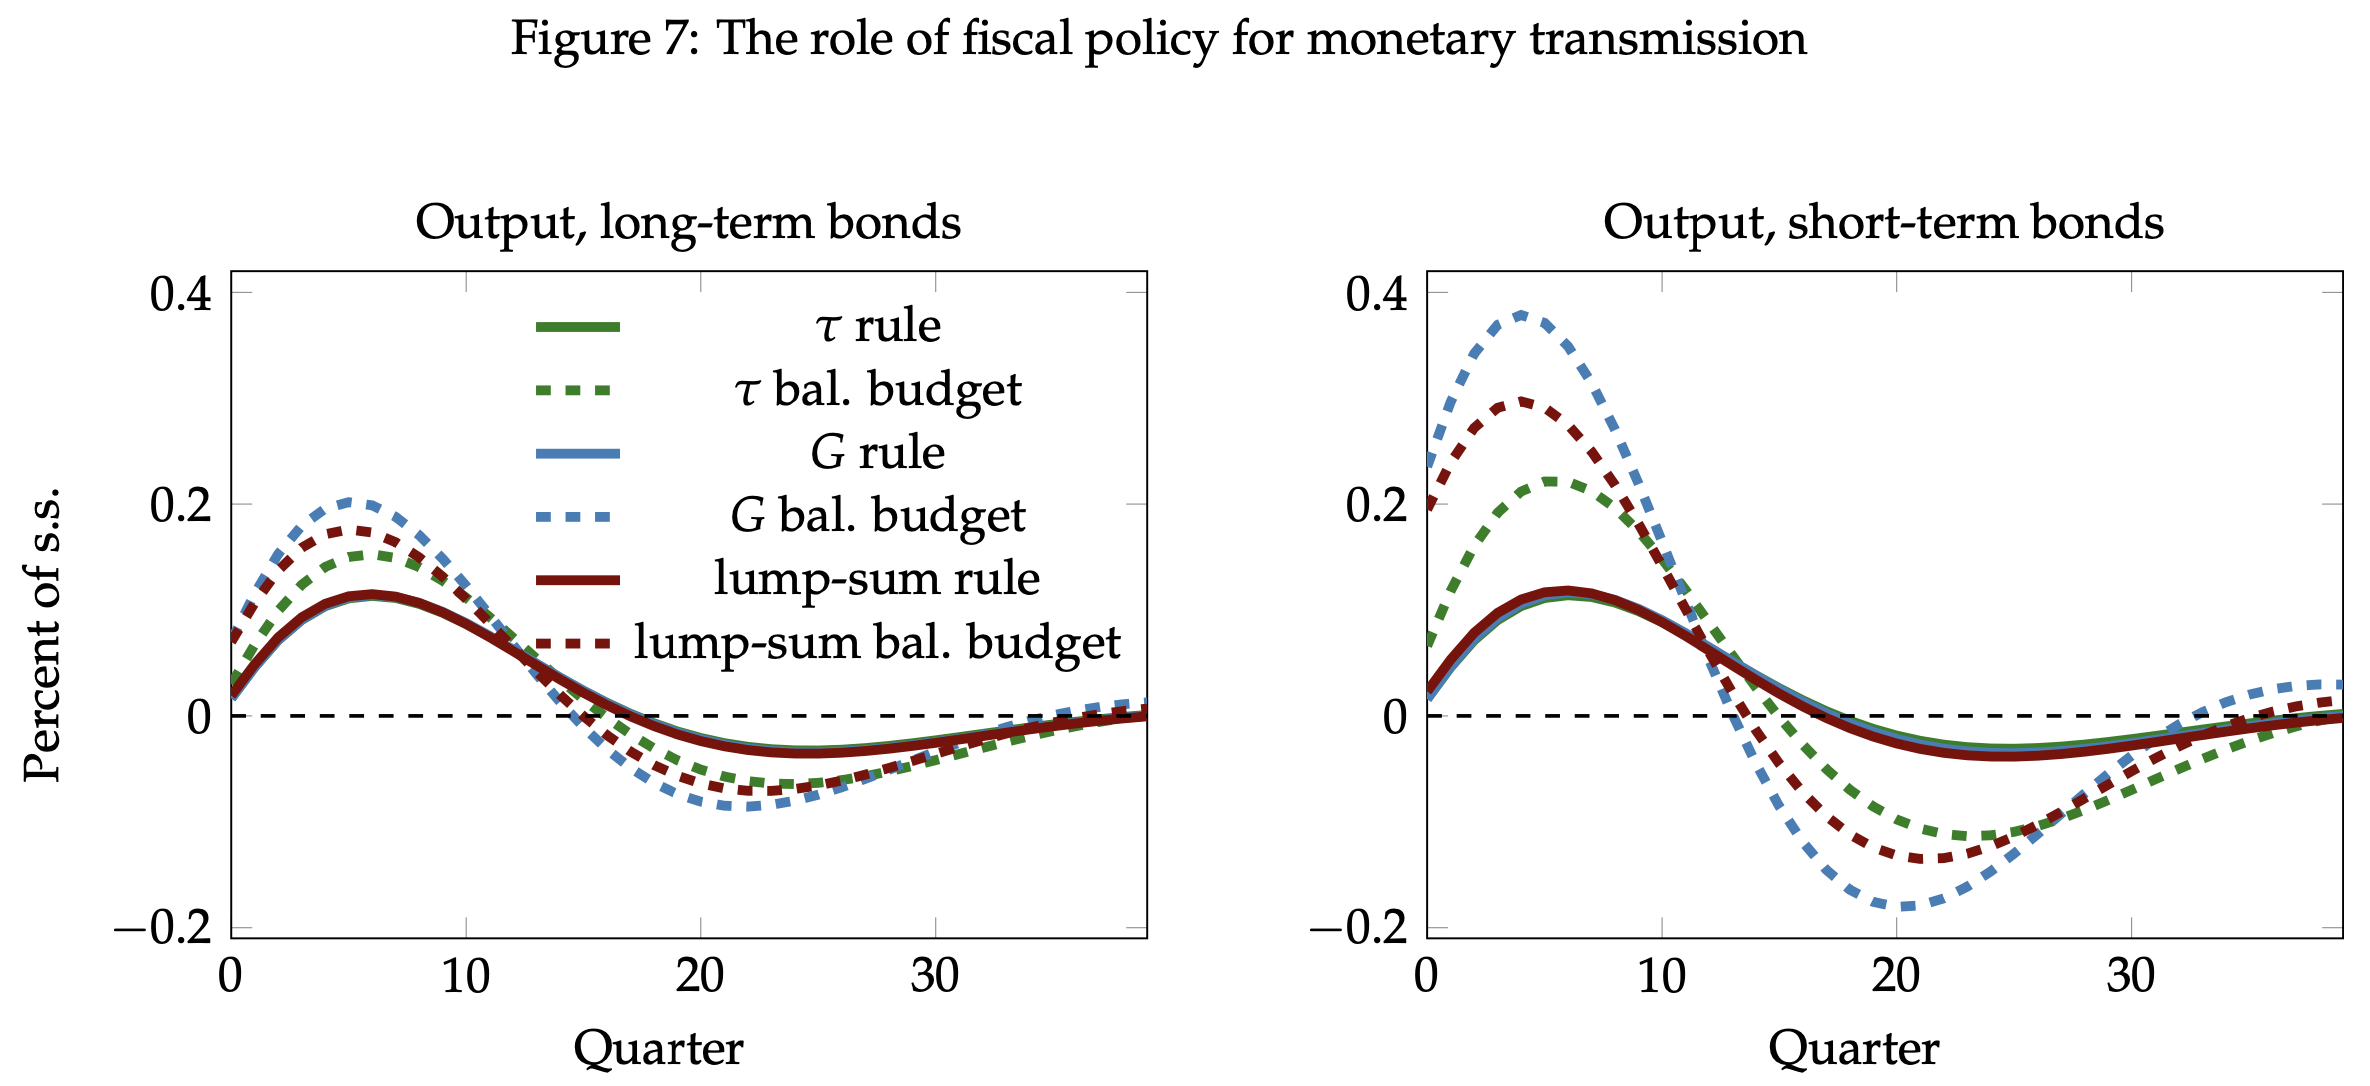
\includegraphics[scale=0.25]{figures/ARSFIG7.png}	
    \end{center}
\end{frame}

\begin{frame}
    \frametitle{Starting the Transmission Mechanism}
    \begin{center}
    	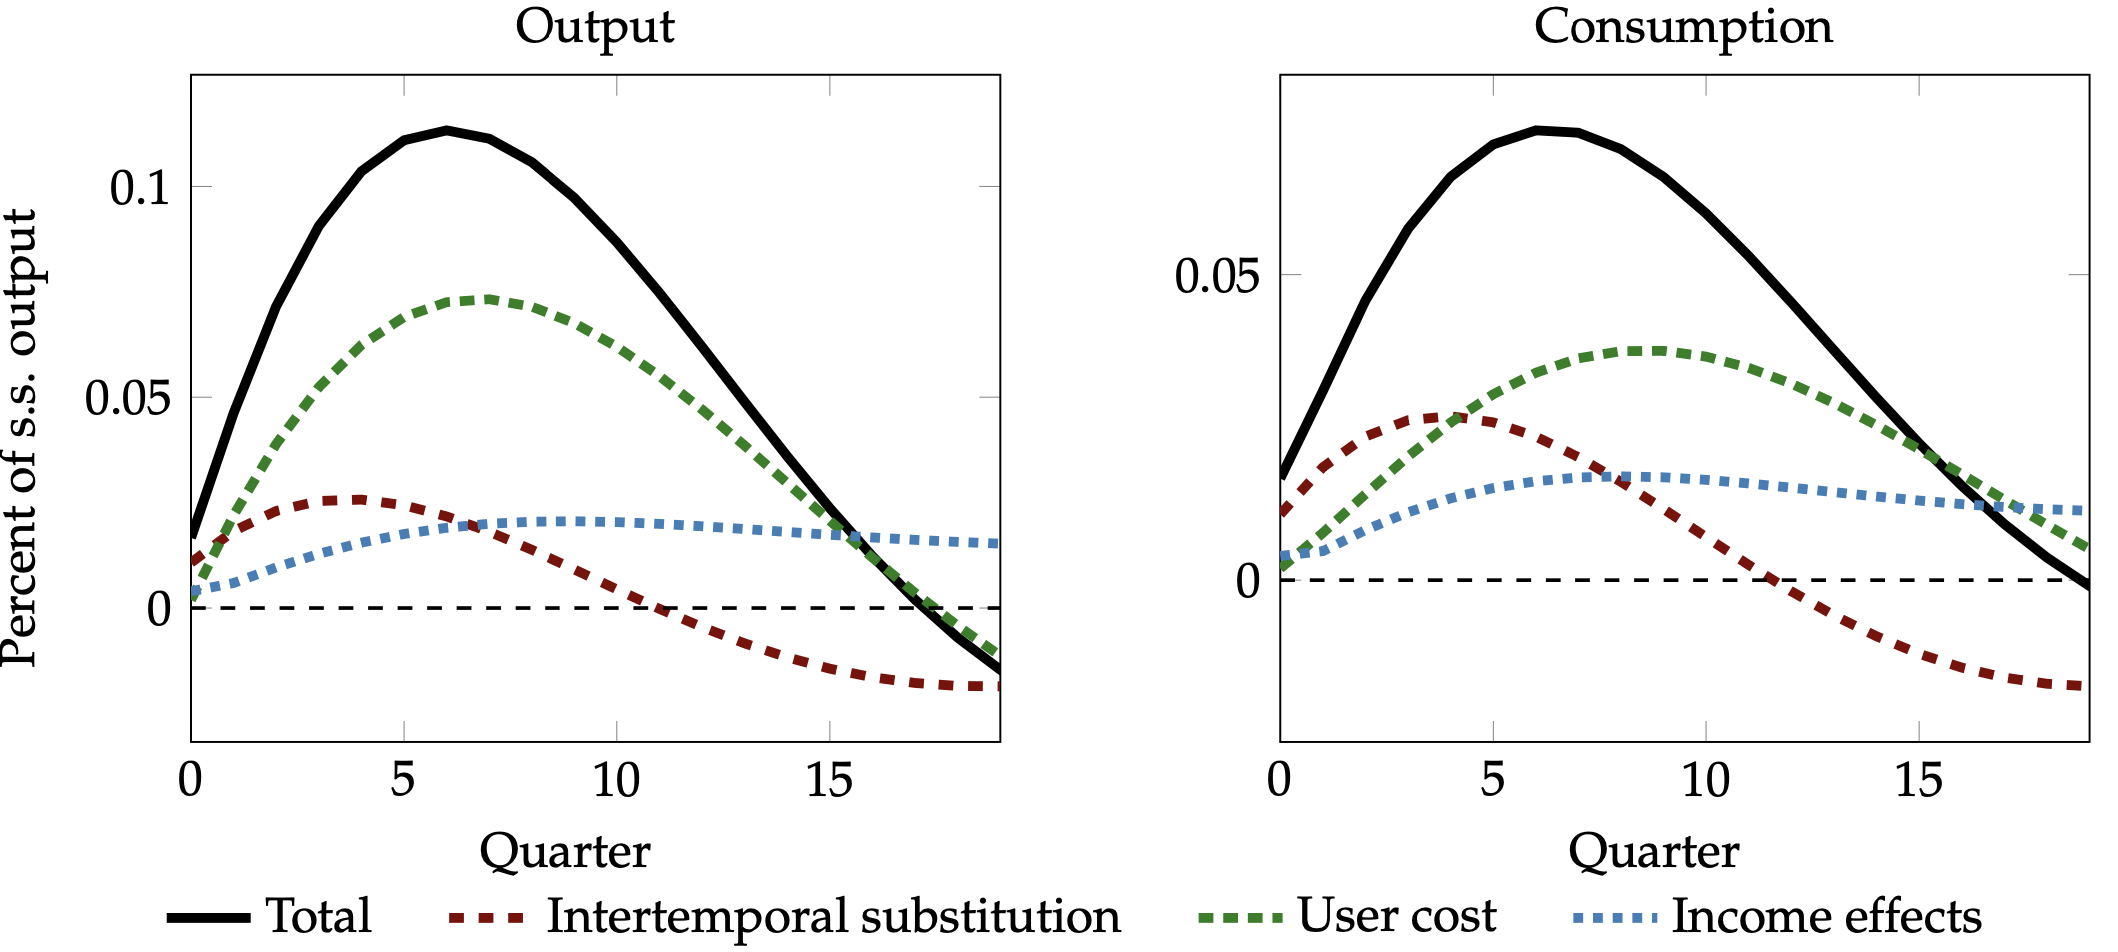
\includegraphics[scale=0.3]{figures/ARSFIG8.png}	
    \end{center}
\end{frame}


\begin{frame}
    \frametitle{Reassessing the Importance of Investment}
    \begin{center}
    	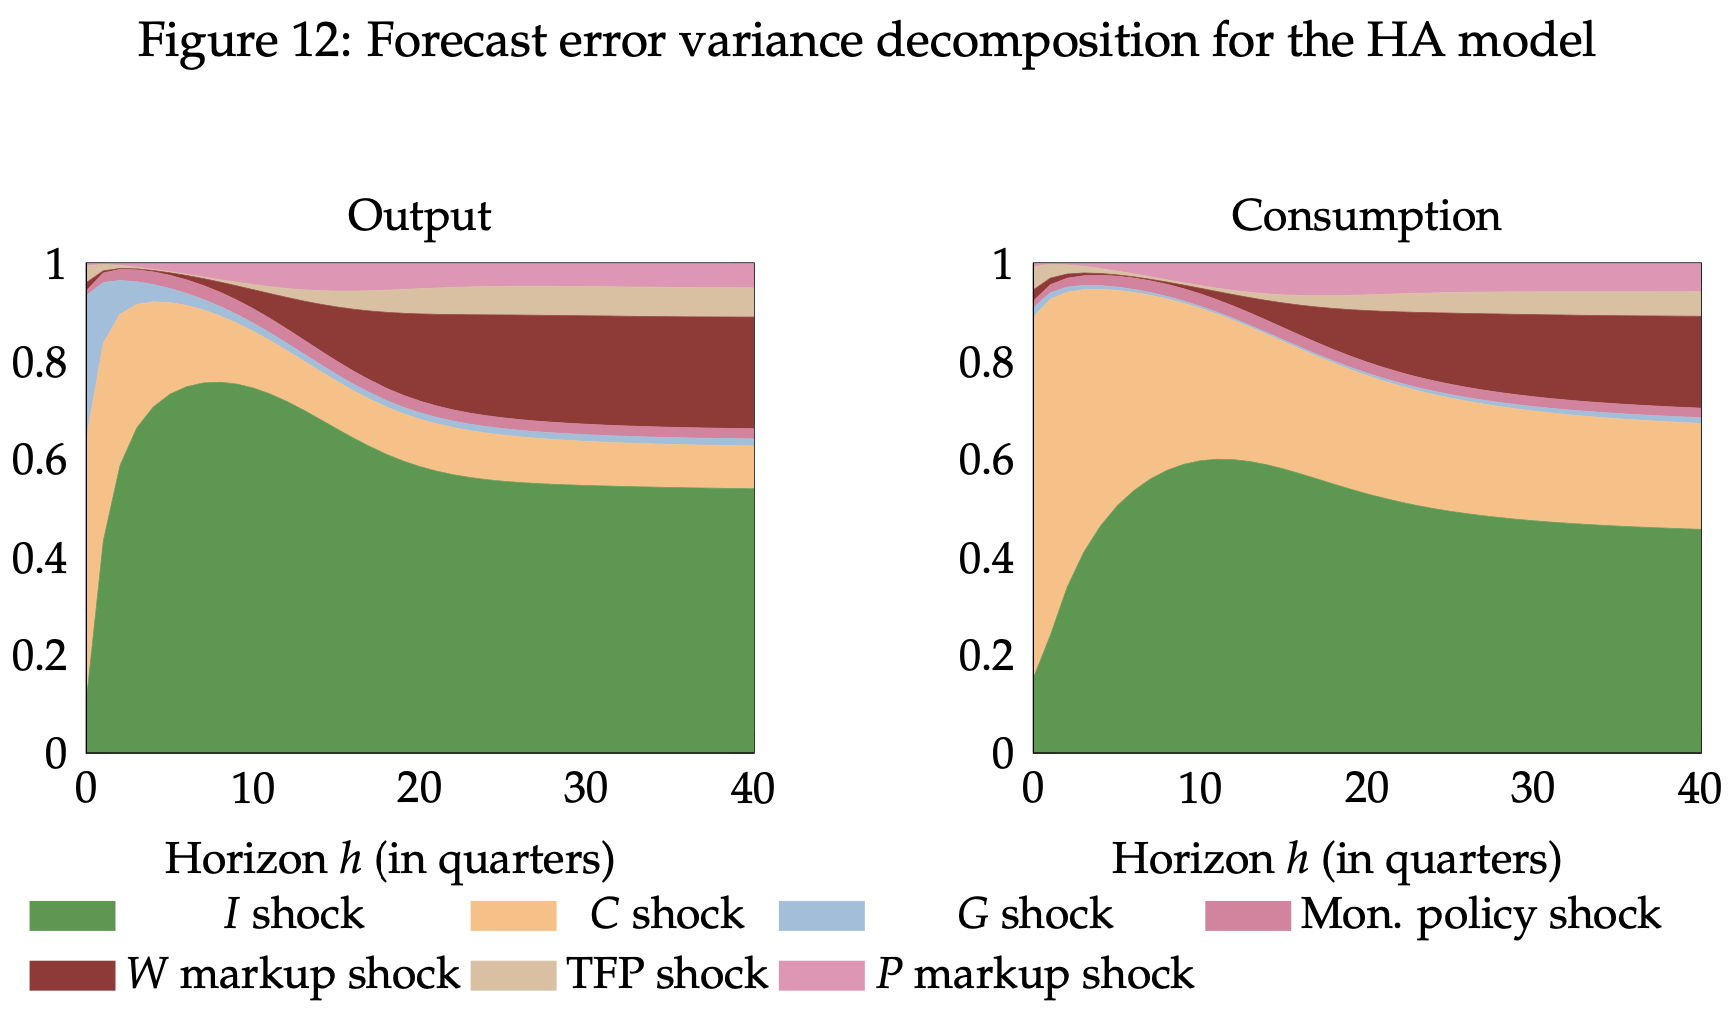
\includegraphics[scale=0.3]{figures/ARSFIG12.png}	
    \end{center}
\end{frame}




%%%%%%%%%%%%%%%%%%%%%%%%%%%%%%%%%%%%%%%%%%%%%%%%%%
\section{Berger, Milbradt, Tourre, Vavra (2021)}
%%%%%%%%%%%%%%%%%%%%%%%%%%%%%%%%%%%%%%%%%%%%%%%%%%



\begin{frame}
    \frametitle{Policy Space}
    \begin{itemize}
    	\item With ZLB constraining $i_t \ge 0$ (or small negative number), central banks can only lower interest rates a finite amount.
    	\item This means that central bank can only offset an AD shock of finite size. This is the ``policy space'' or ``limited ammunition.''
    	\item This paper: when lower interest rates today, then also reduce \emph{responsiveness} to future interest rate changes (up or down).
    	\item Means that past interest rate cuts limit future policy face as subsequent interest rate cuts less effective.
    \end{itemize}
\end{frame}


\begin{frame}
    \frametitle{Refinancing (Pre-payment)}
    \begin{itemize}
    	\item Estimate effect of rate gap on refinancing probability.
    	\begin{align*}
    	prepay_{i,j,t} = \beta_{gapbin} \bm{1}(gapbin)_{j,t} + \beta_X X_{i,j,t} + \delta_i + \epsilon_{i,j,t}
    \end{align*}
    \item Identification assumption?
    \end{itemize}
\end{frame}

\begin{frame}
    \frametitle{Refinancing (Pre-payment)}
    \begin{center}
    	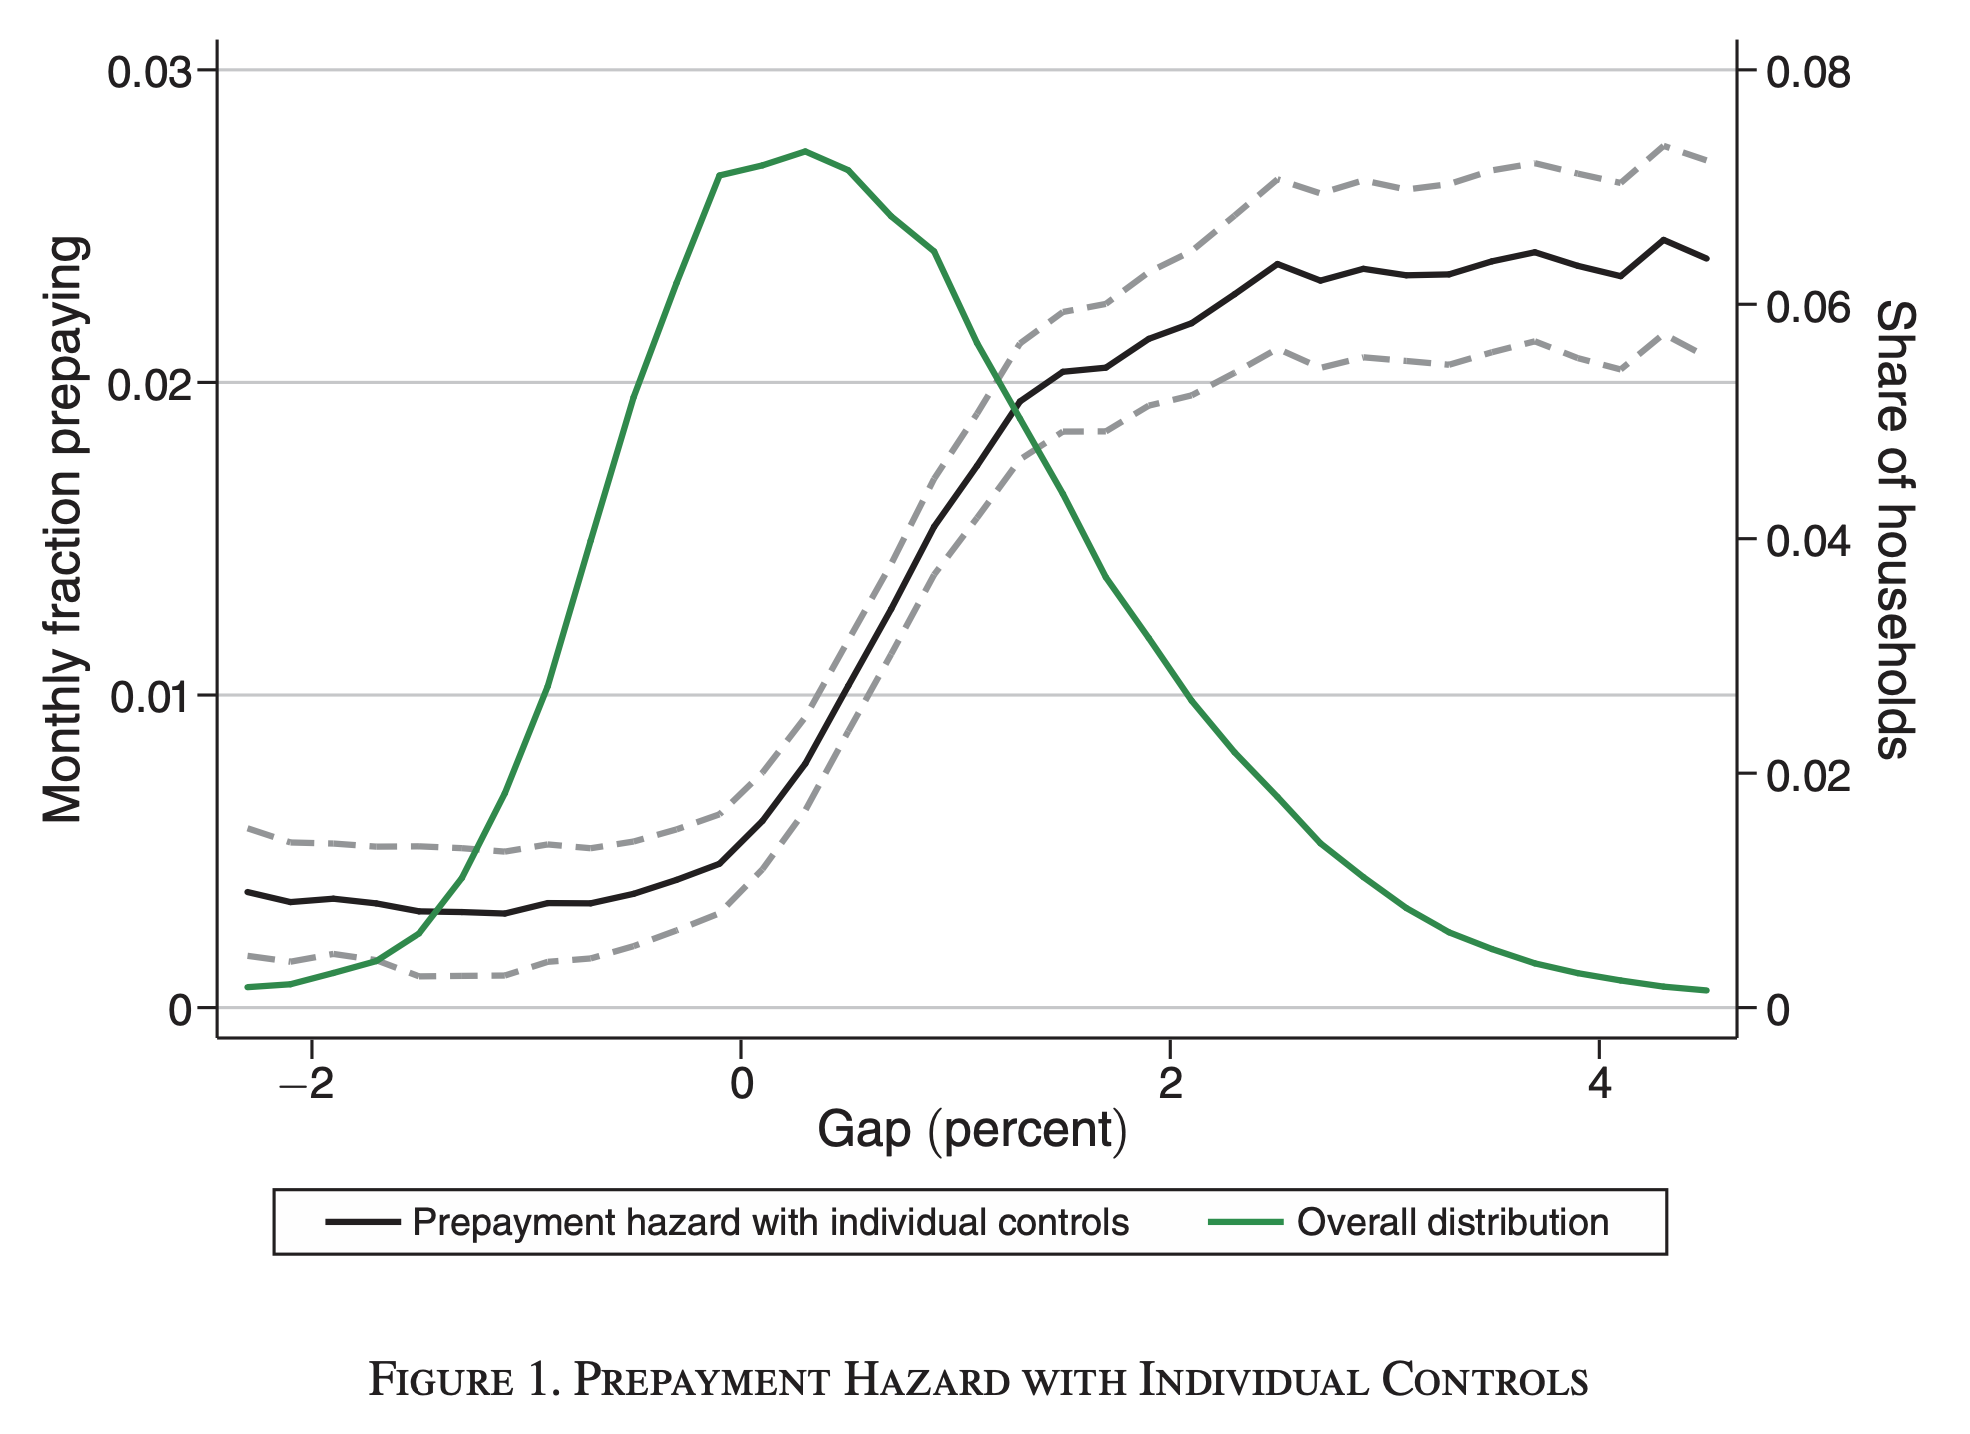
\includegraphics[scale=0.3]{figures/BMTVFIG1.png}	
    \end{center}
\end{frame}

\begin{frame}
    \frametitle{Motives}
    \begin{center}
    	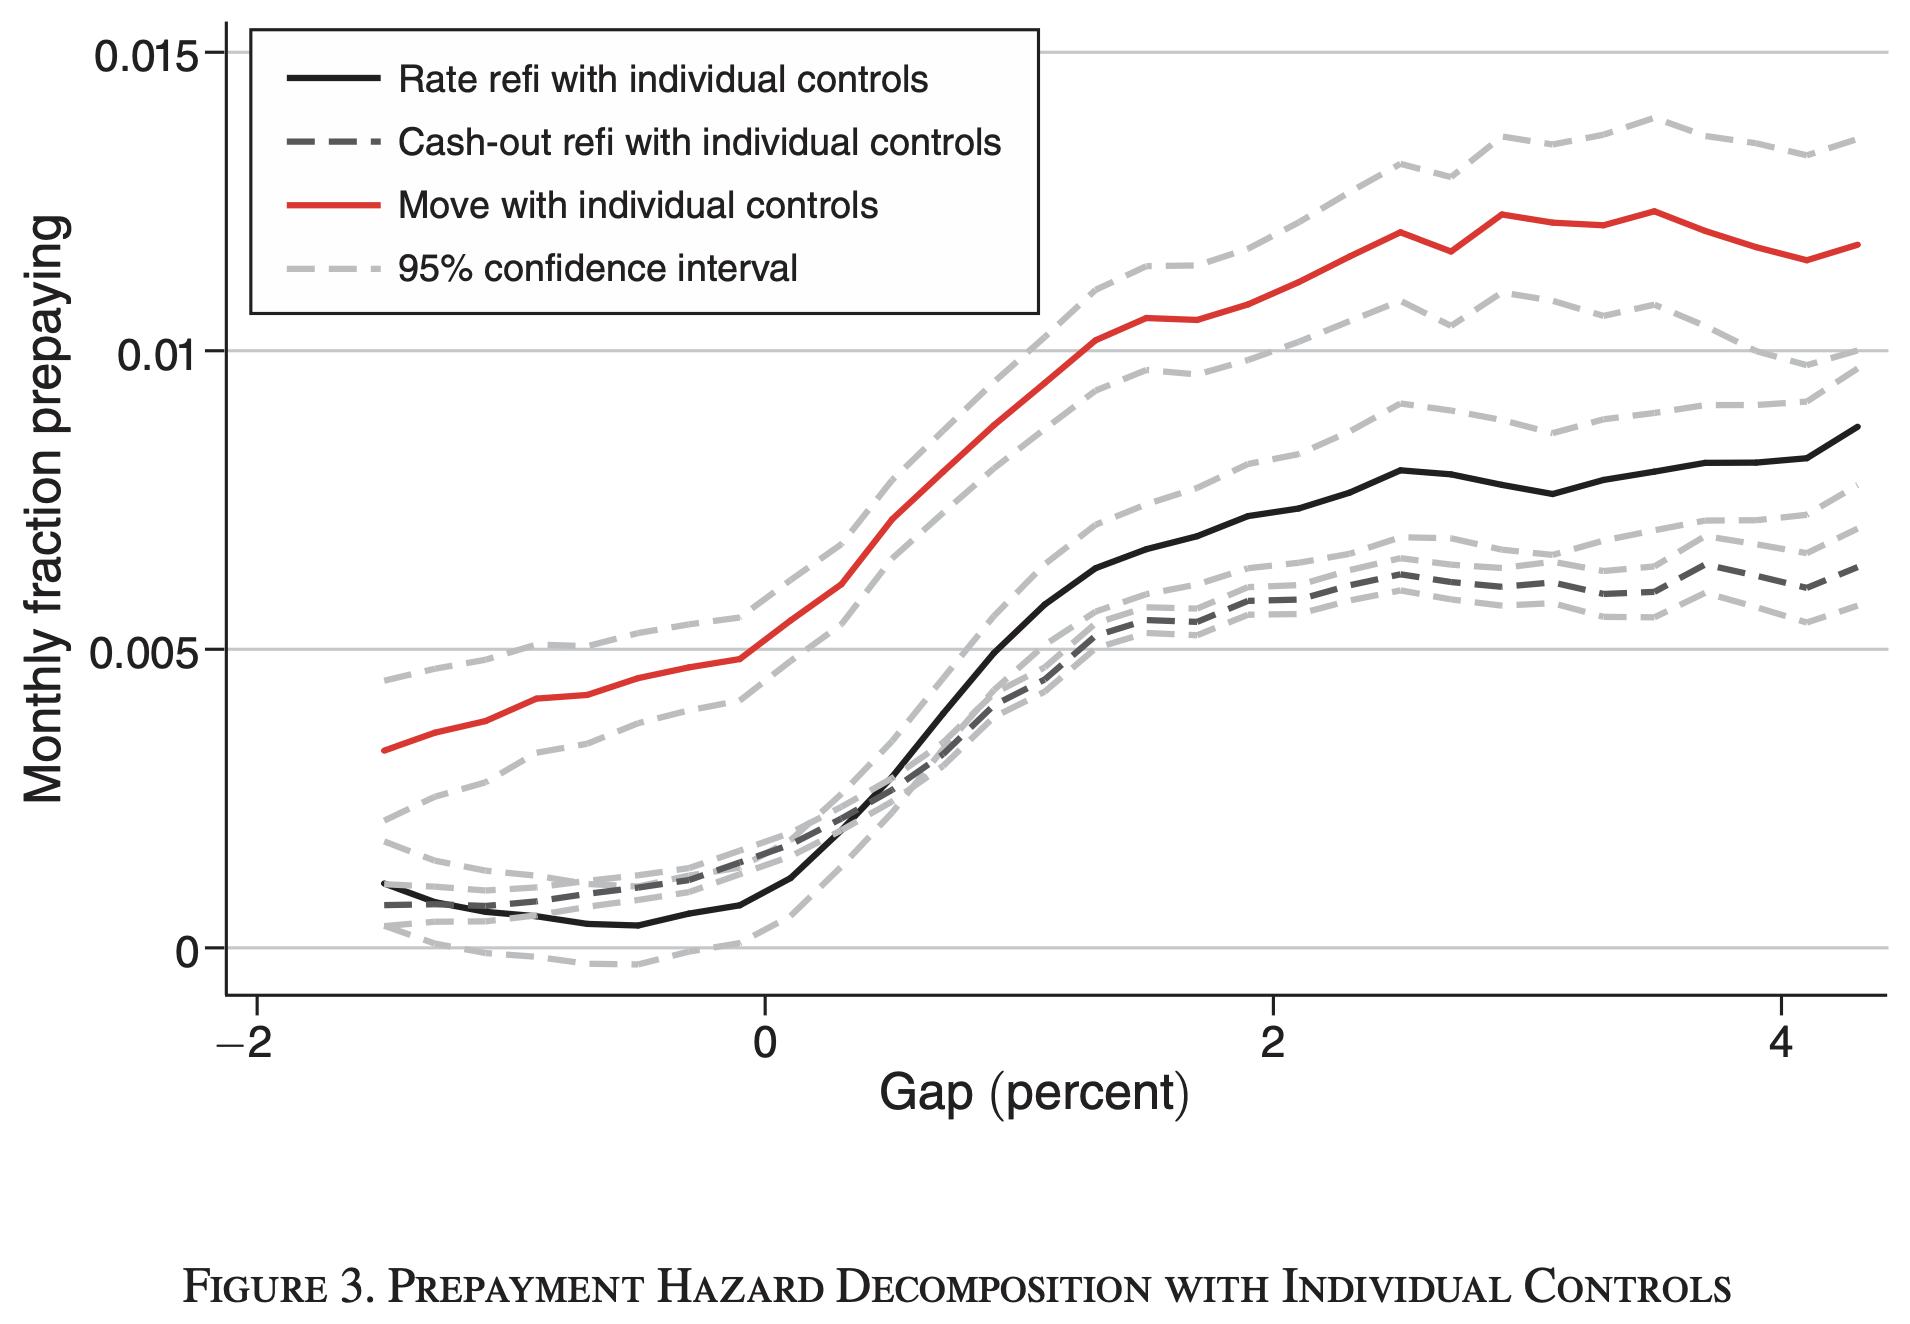
\includegraphics[scale=0.3]{figures/BMTVFIG3.png}	
    \end{center}
\end{frame}

\begin{frame}
    \frametitle{Aggregate Correlation}
    \begin{center}
    	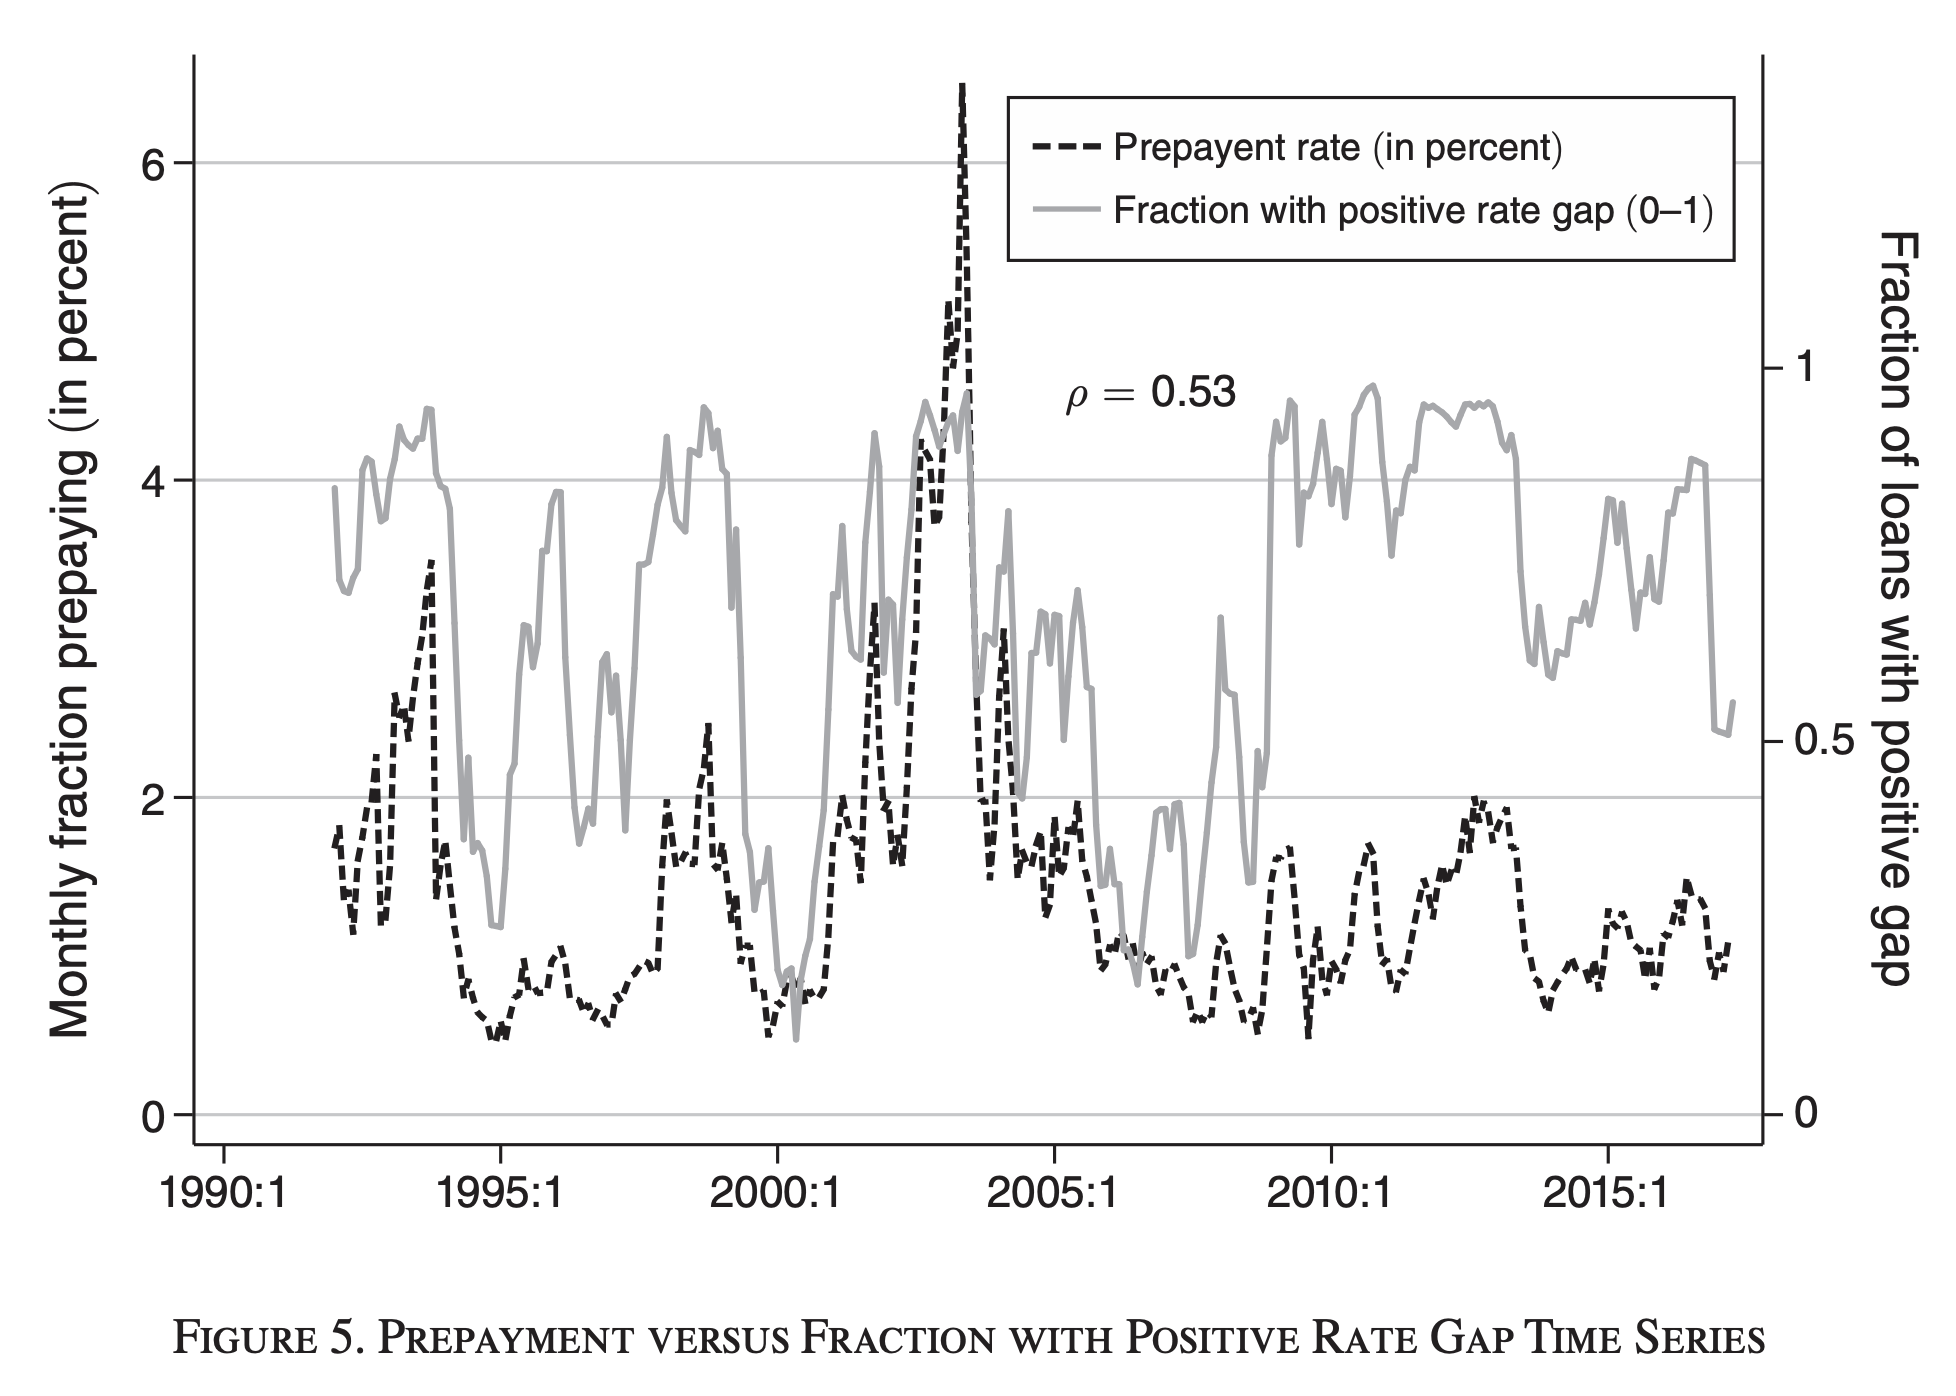
\includegraphics[scale=0.3]{figures/BMTVFIG4.png}	
    \end{center}
\end{frame}

\begin{frame}
    \frametitle{Spending}
    \begin{itemize}
    	\item Estimate effect of refinancing probability on spending.
    	\begin{align*}
    	\bm{1}(carloan)_{i,t} = \sum_k \bm{1}(refinanced)_{i,t-k}  + \delta_i + \delta_t + \epsilon_{i,t}
    \end{align*}
    \item Identification assumption?
    \end{itemize}
\end{frame}


\begin{frame}
    \frametitle{Spending}
    \begin{center}
    	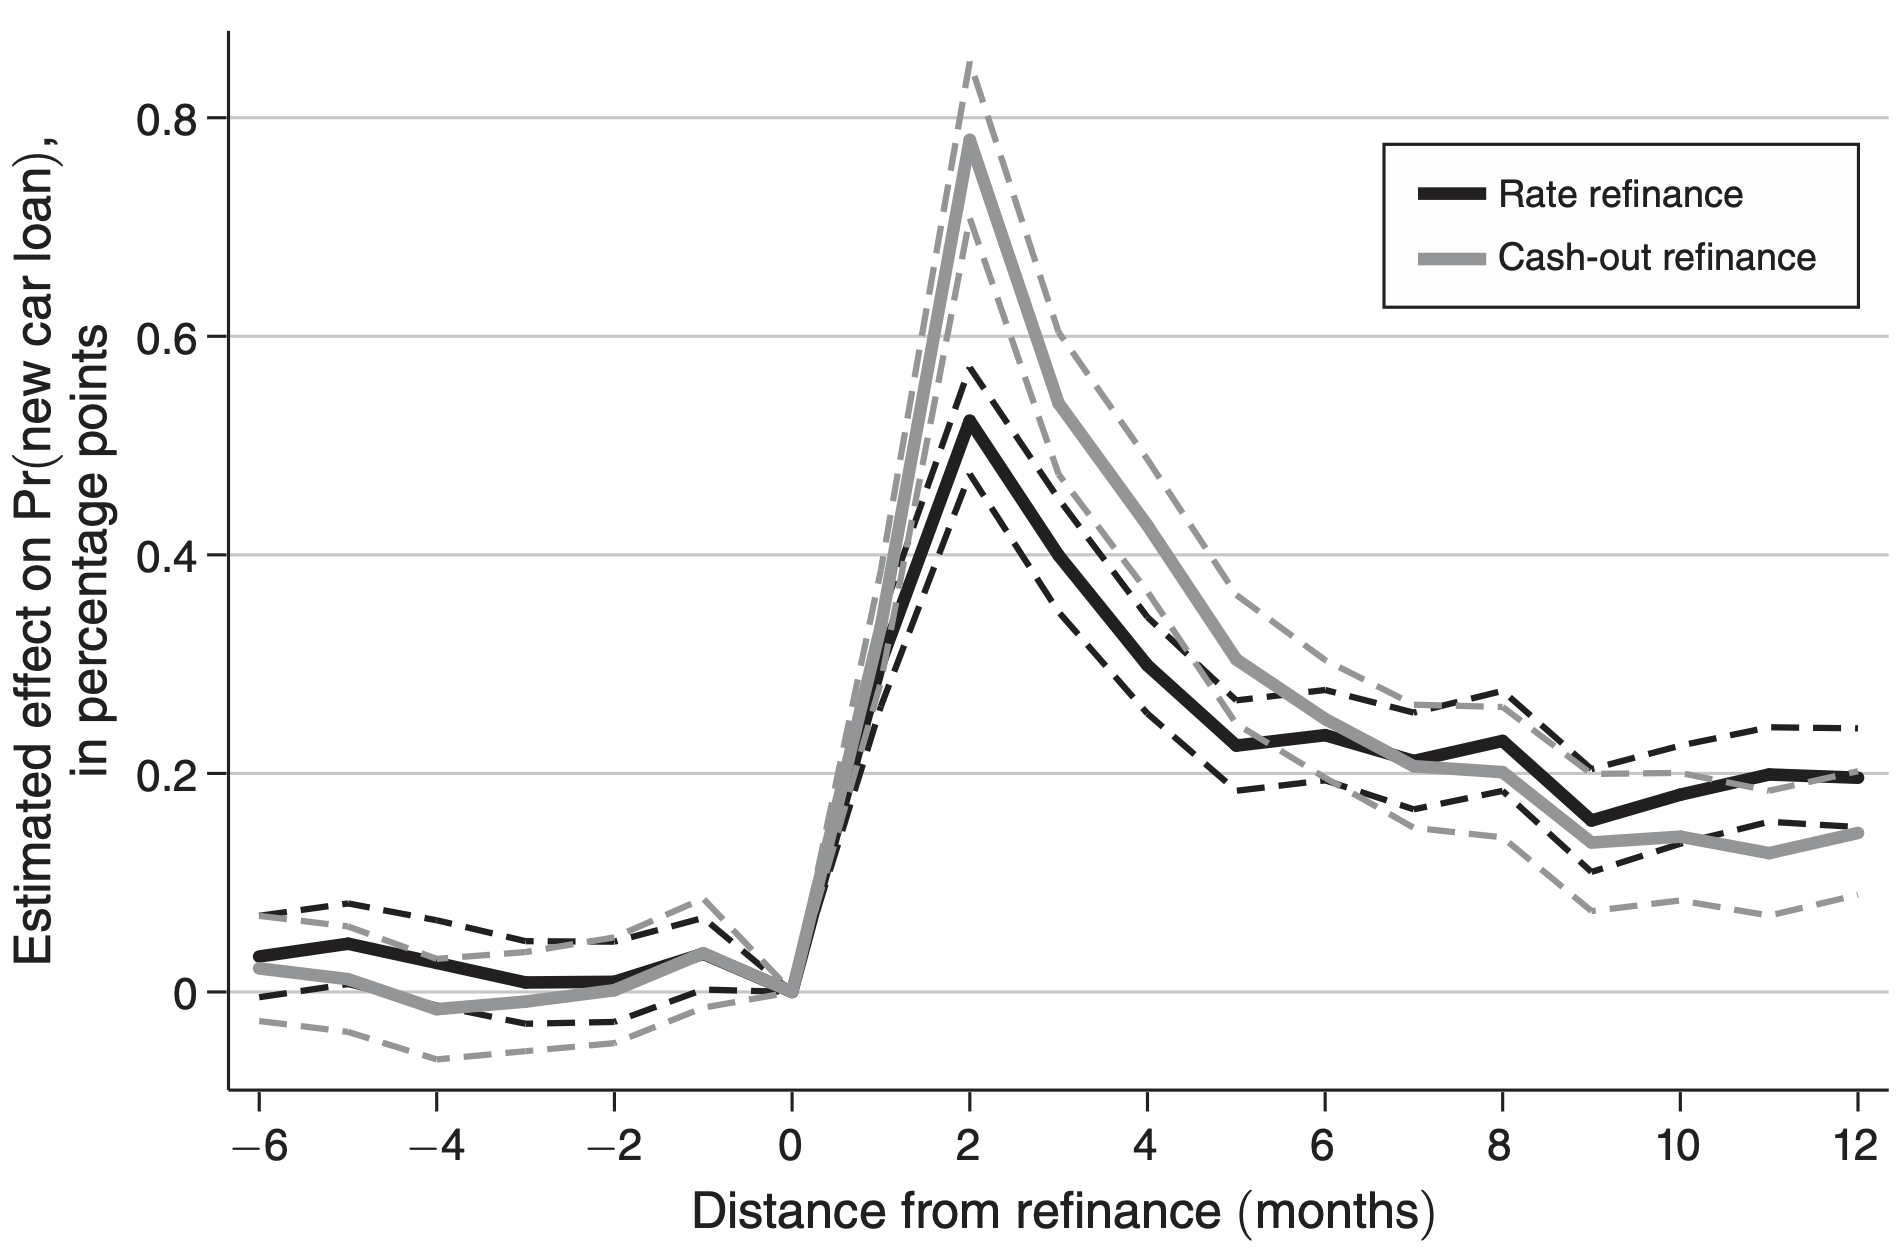
\includegraphics[scale=0.3]{figures/BMTVFIG5.png}	
    \end{center}
\end{frame}

\begin{frame}
    \frametitle{Why Do We Need a Model?}
\end{frame}

\begin{frame}
    \frametitle{Gaps and Frequency}
    \begin{center}
    	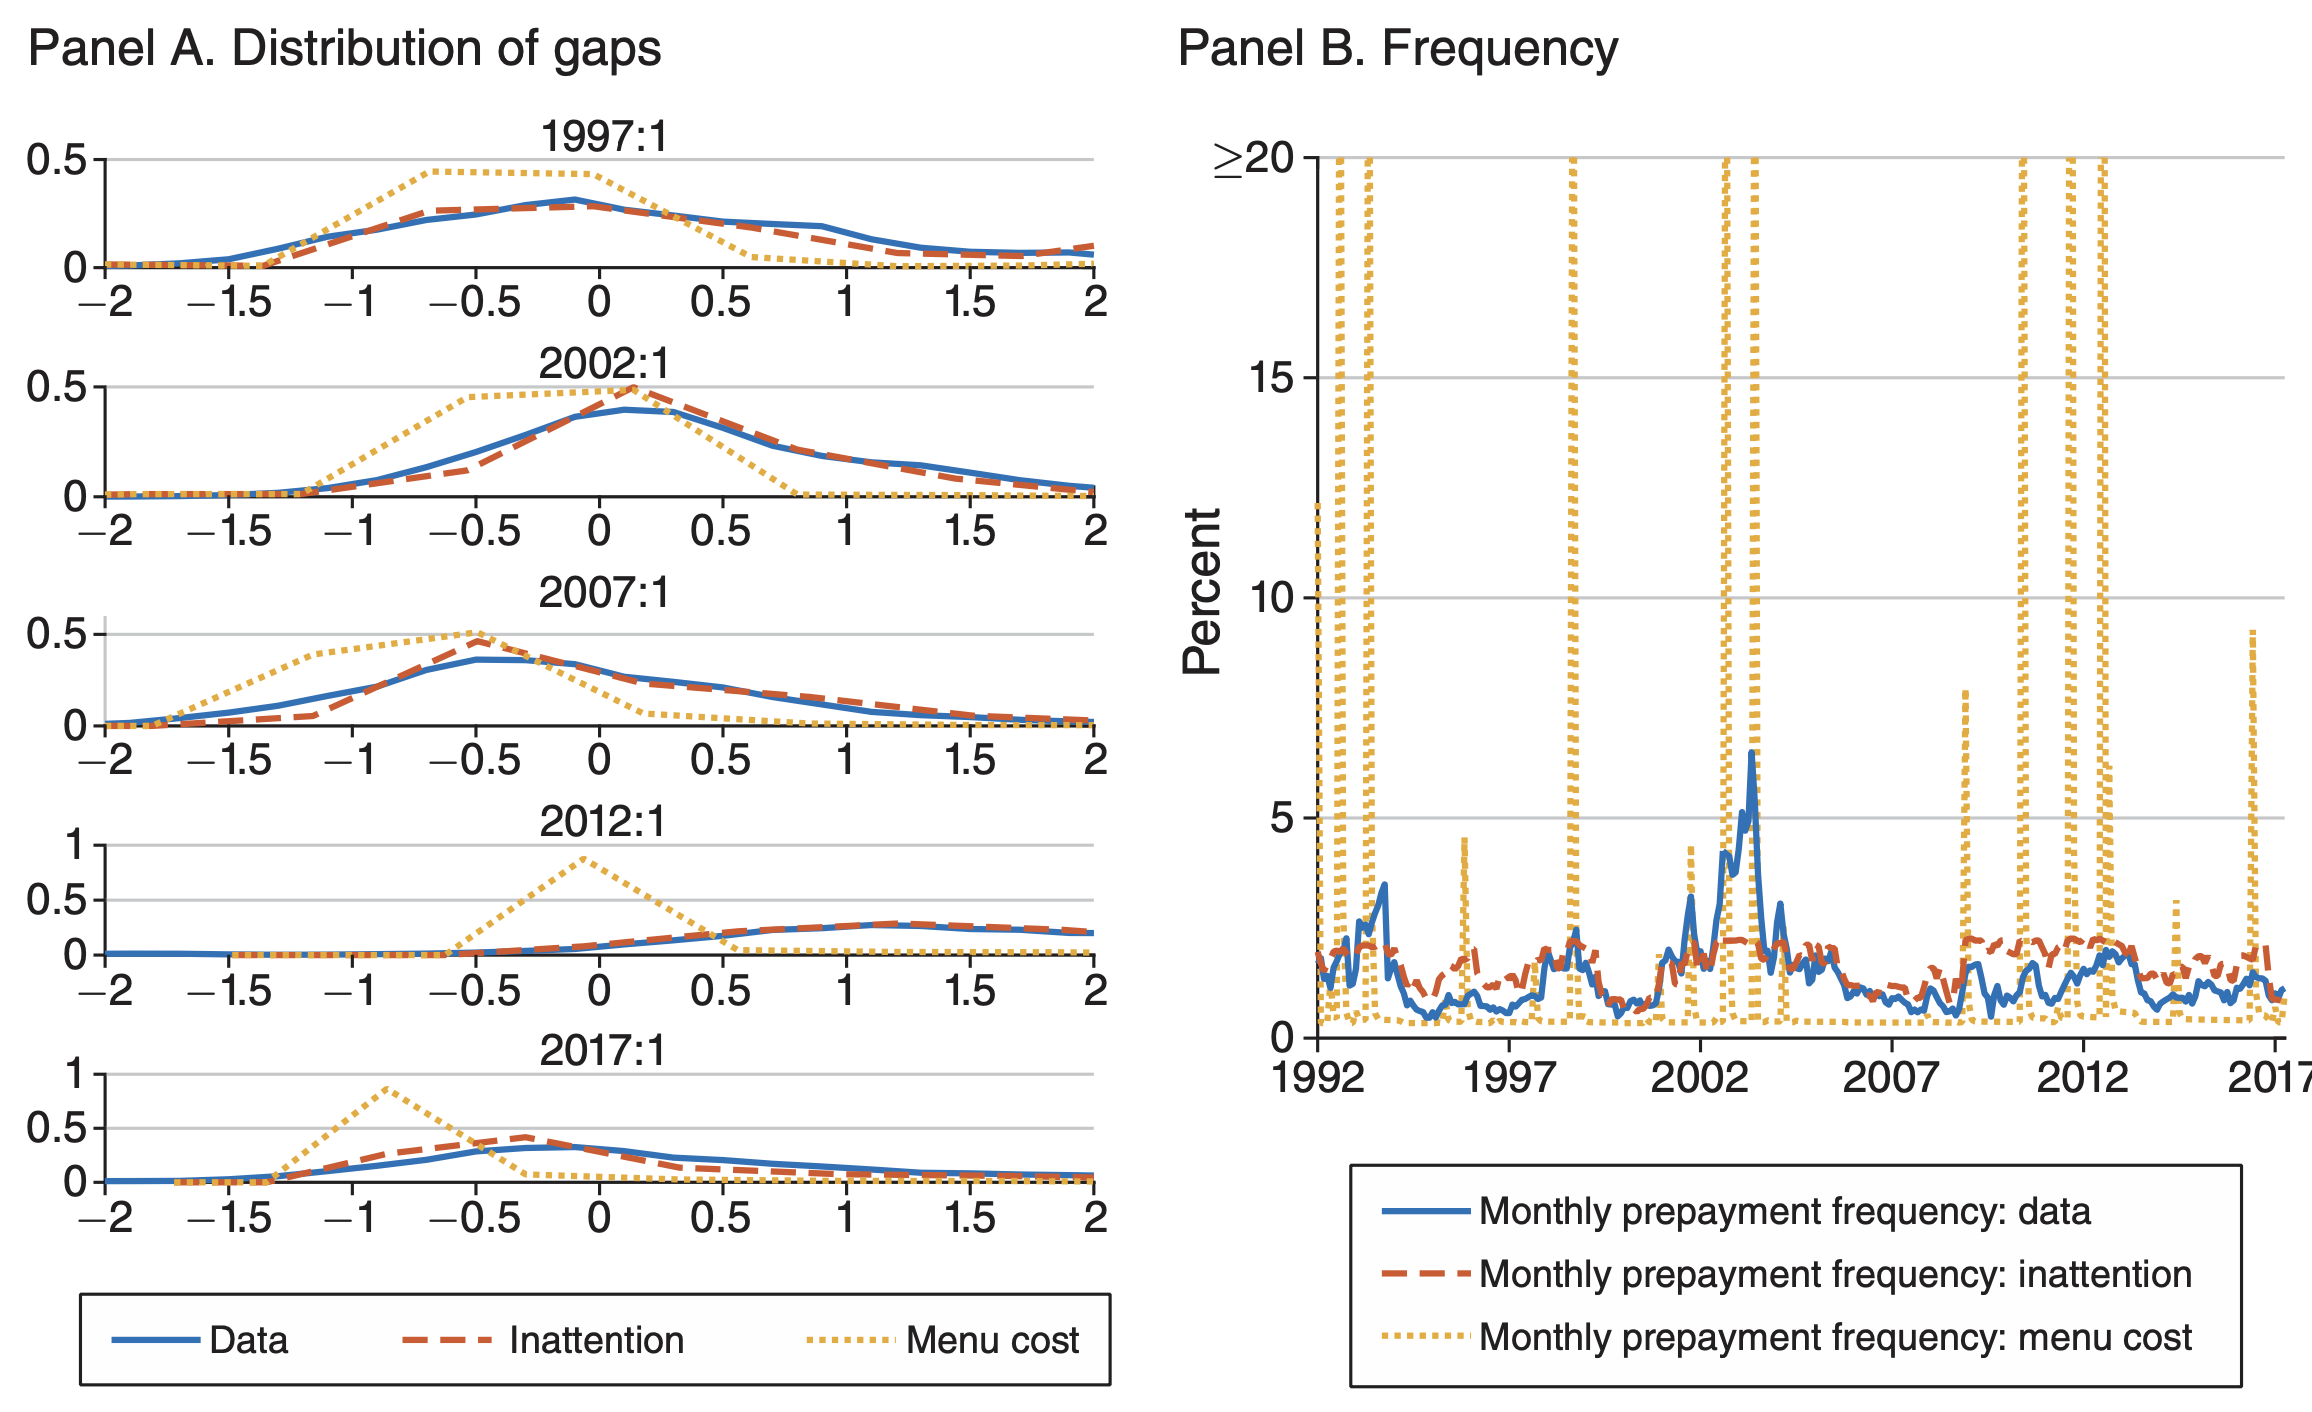
\includegraphics[scale=0.3]{figures/BMTVFIG9AB.png}	
    \end{center}
\end{frame}

\begin{frame}
    \frametitle{Hybrid Model}
    \begin{center}
    	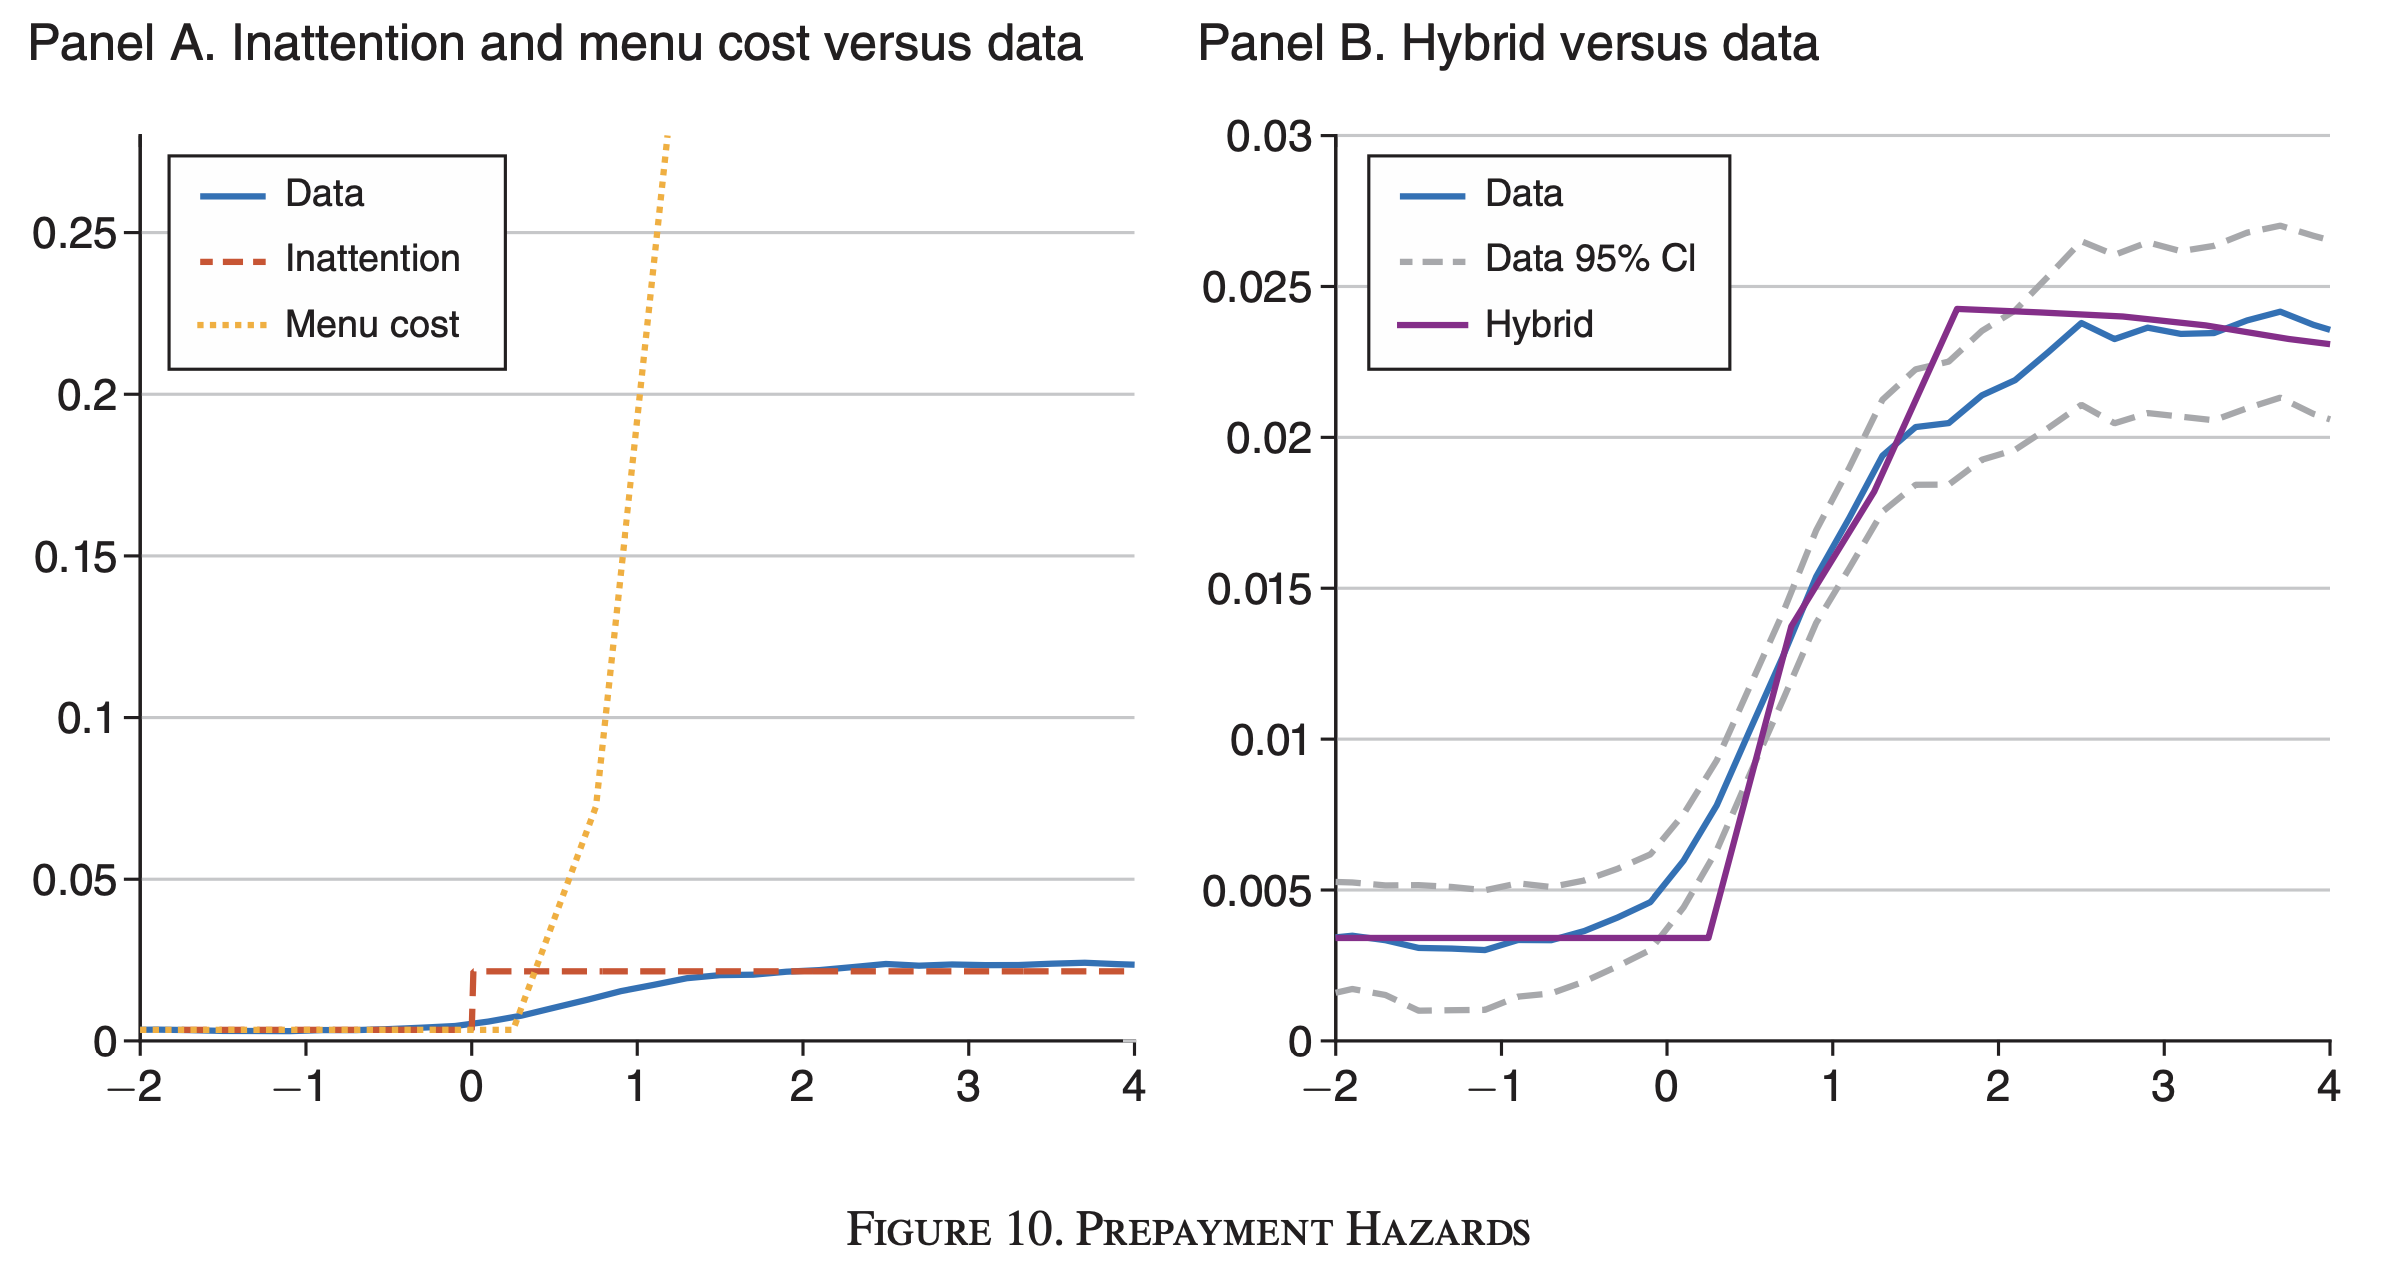
\includegraphics[scale=0.3]{figures/BMTVFIG10.png}	
    \end{center}
\end{frame}


\begin{frame}
    \frametitle{State Dependence}
    \begin{center}
    	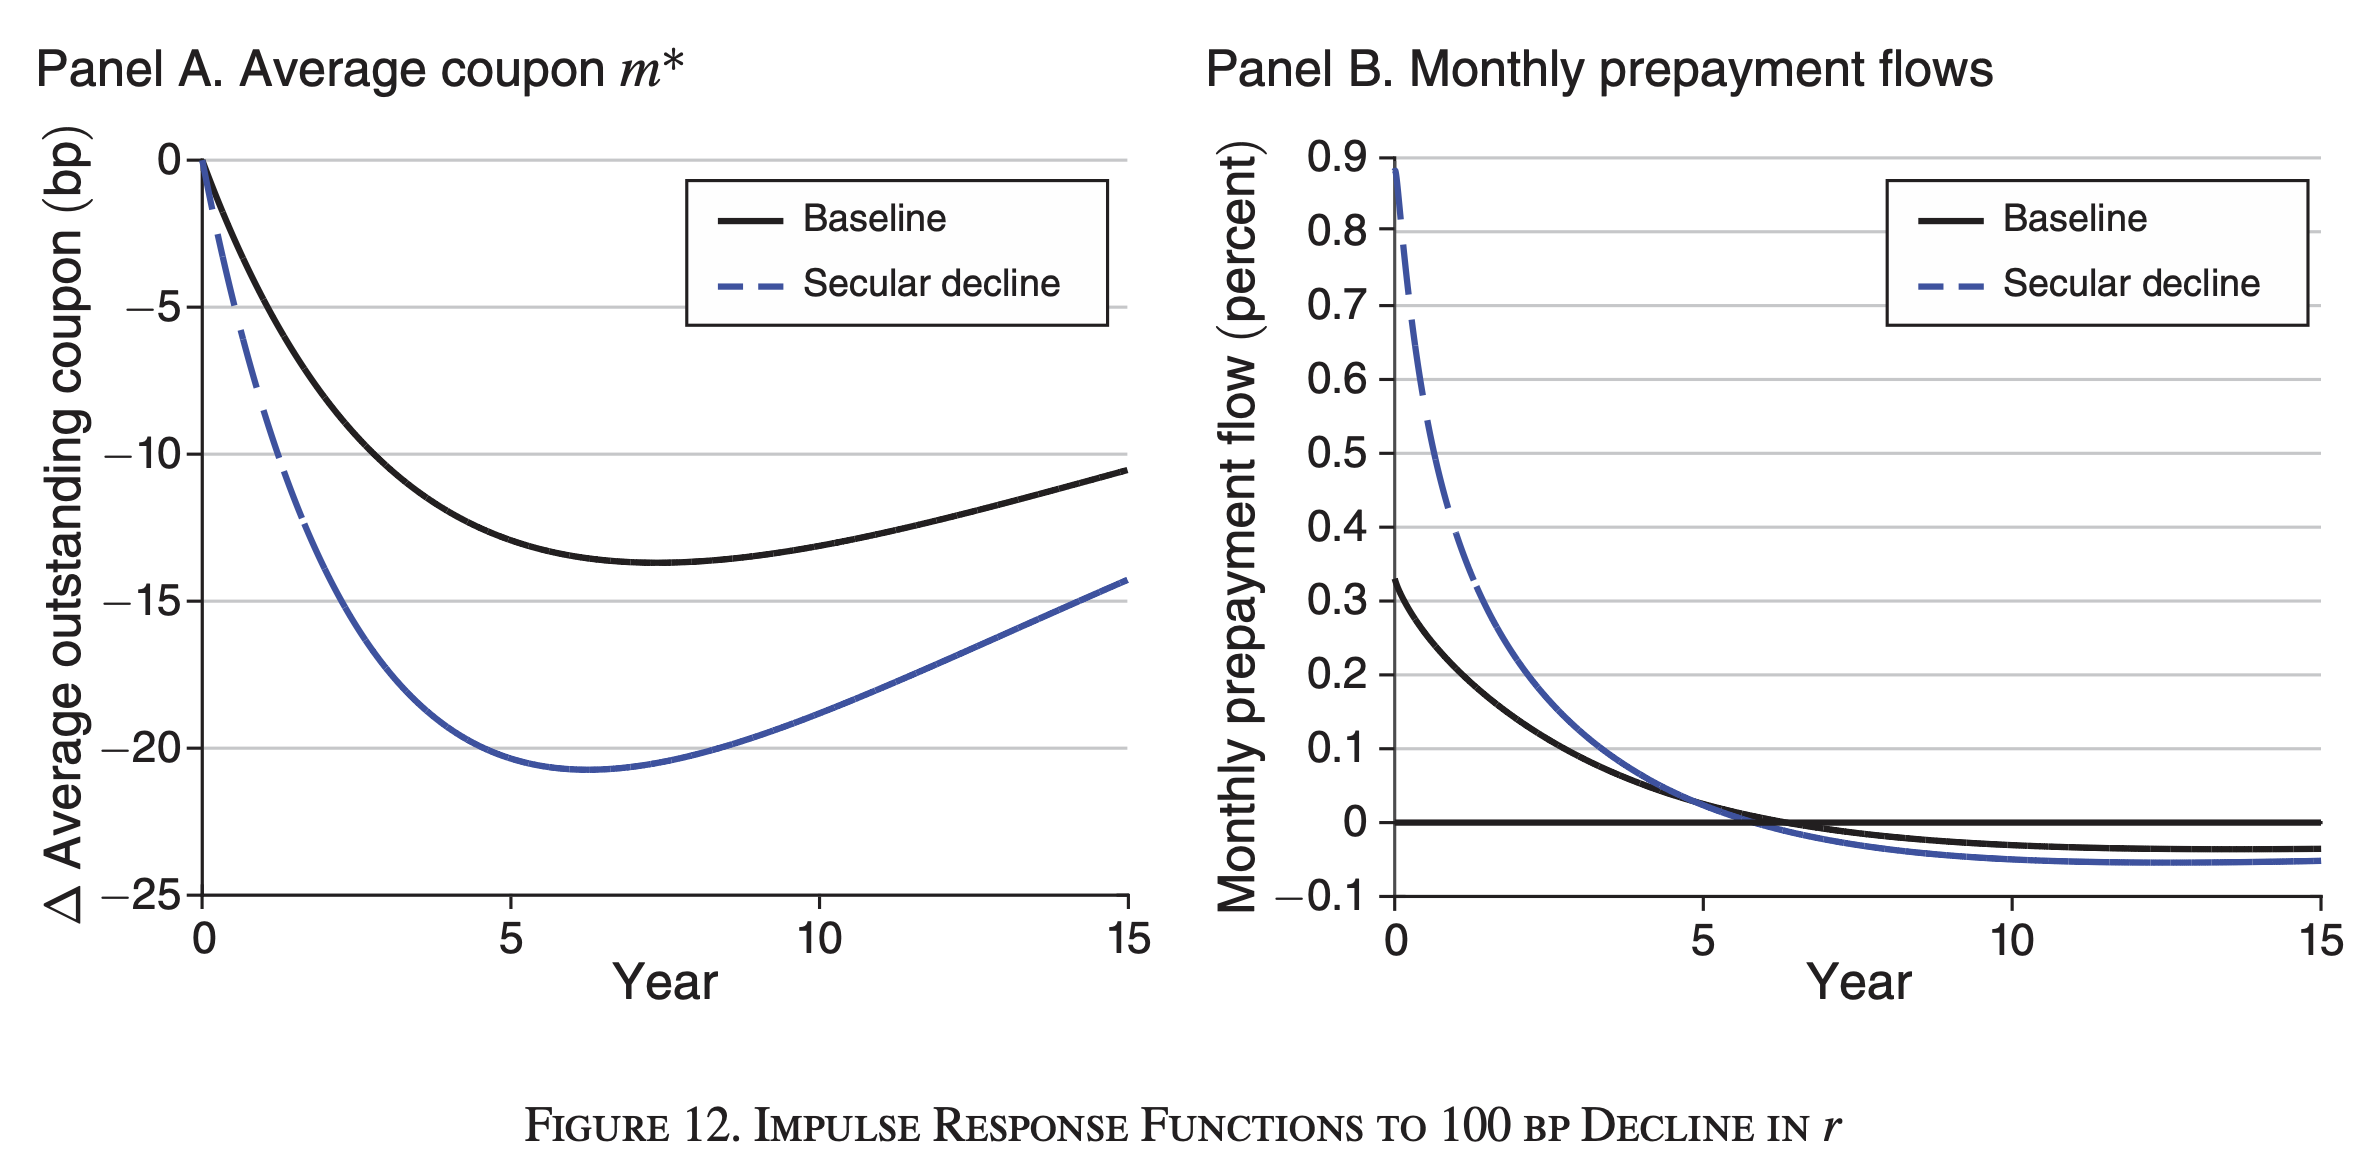
\includegraphics[scale=0.3]{figures/BMTVFIG12.png}	
    \end{center}
\end{frame}

\begin{frame}
    \frametitle{State Dependence}
    \begin{center}
    	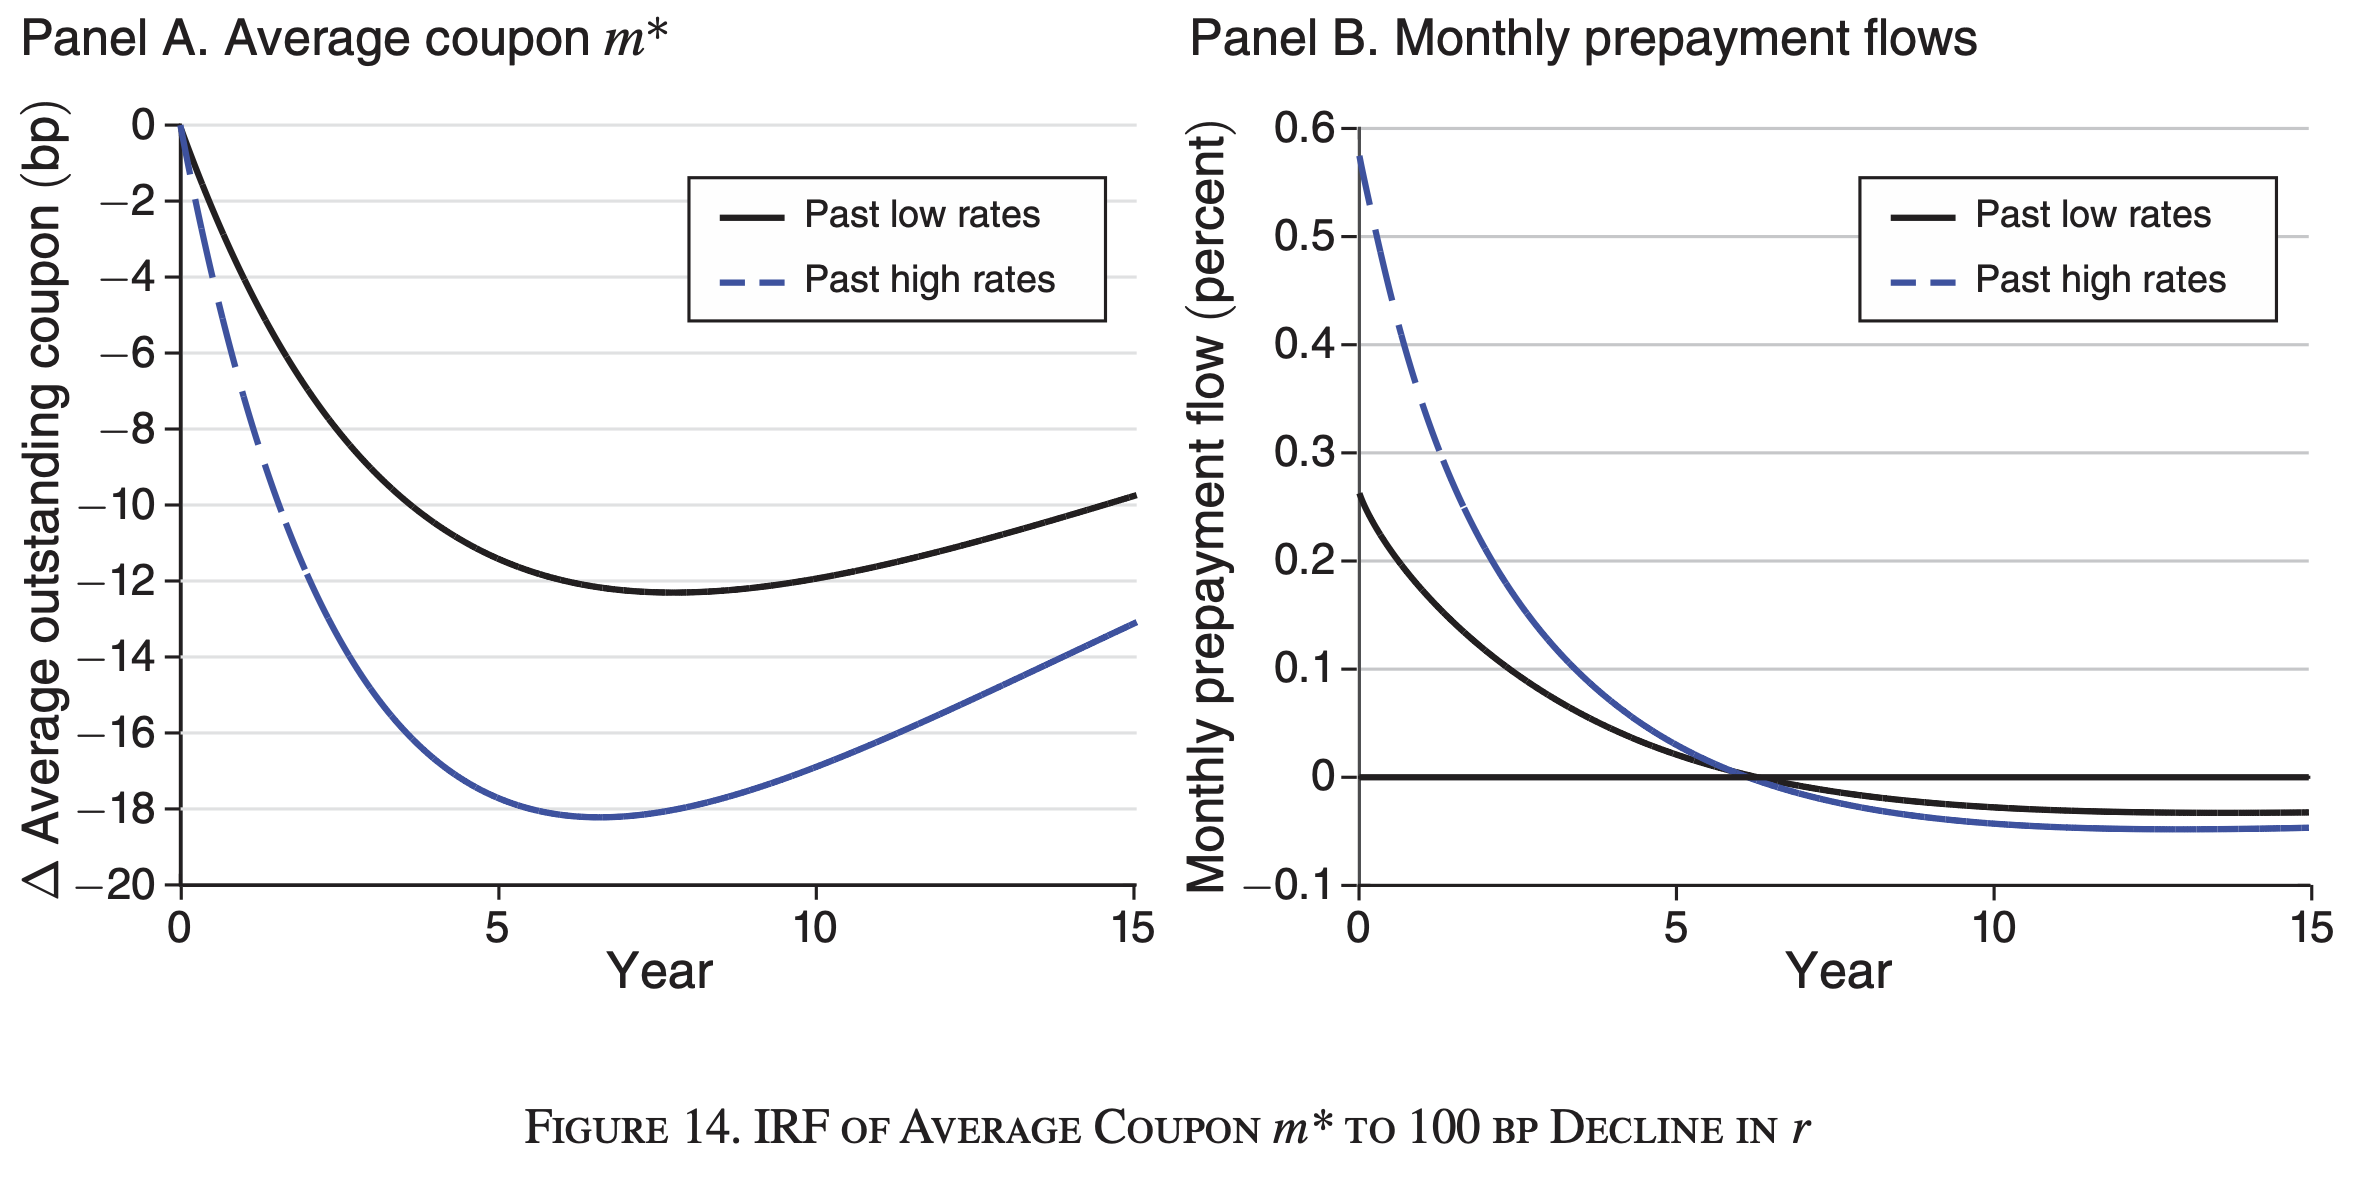
\includegraphics[scale=0.3]{figures/BMTVFIG13.png}	
    \end{center}
\end{frame}

\begin{frame}
    \frametitle{Shift in Policy Stance}
    \begin{center}
    	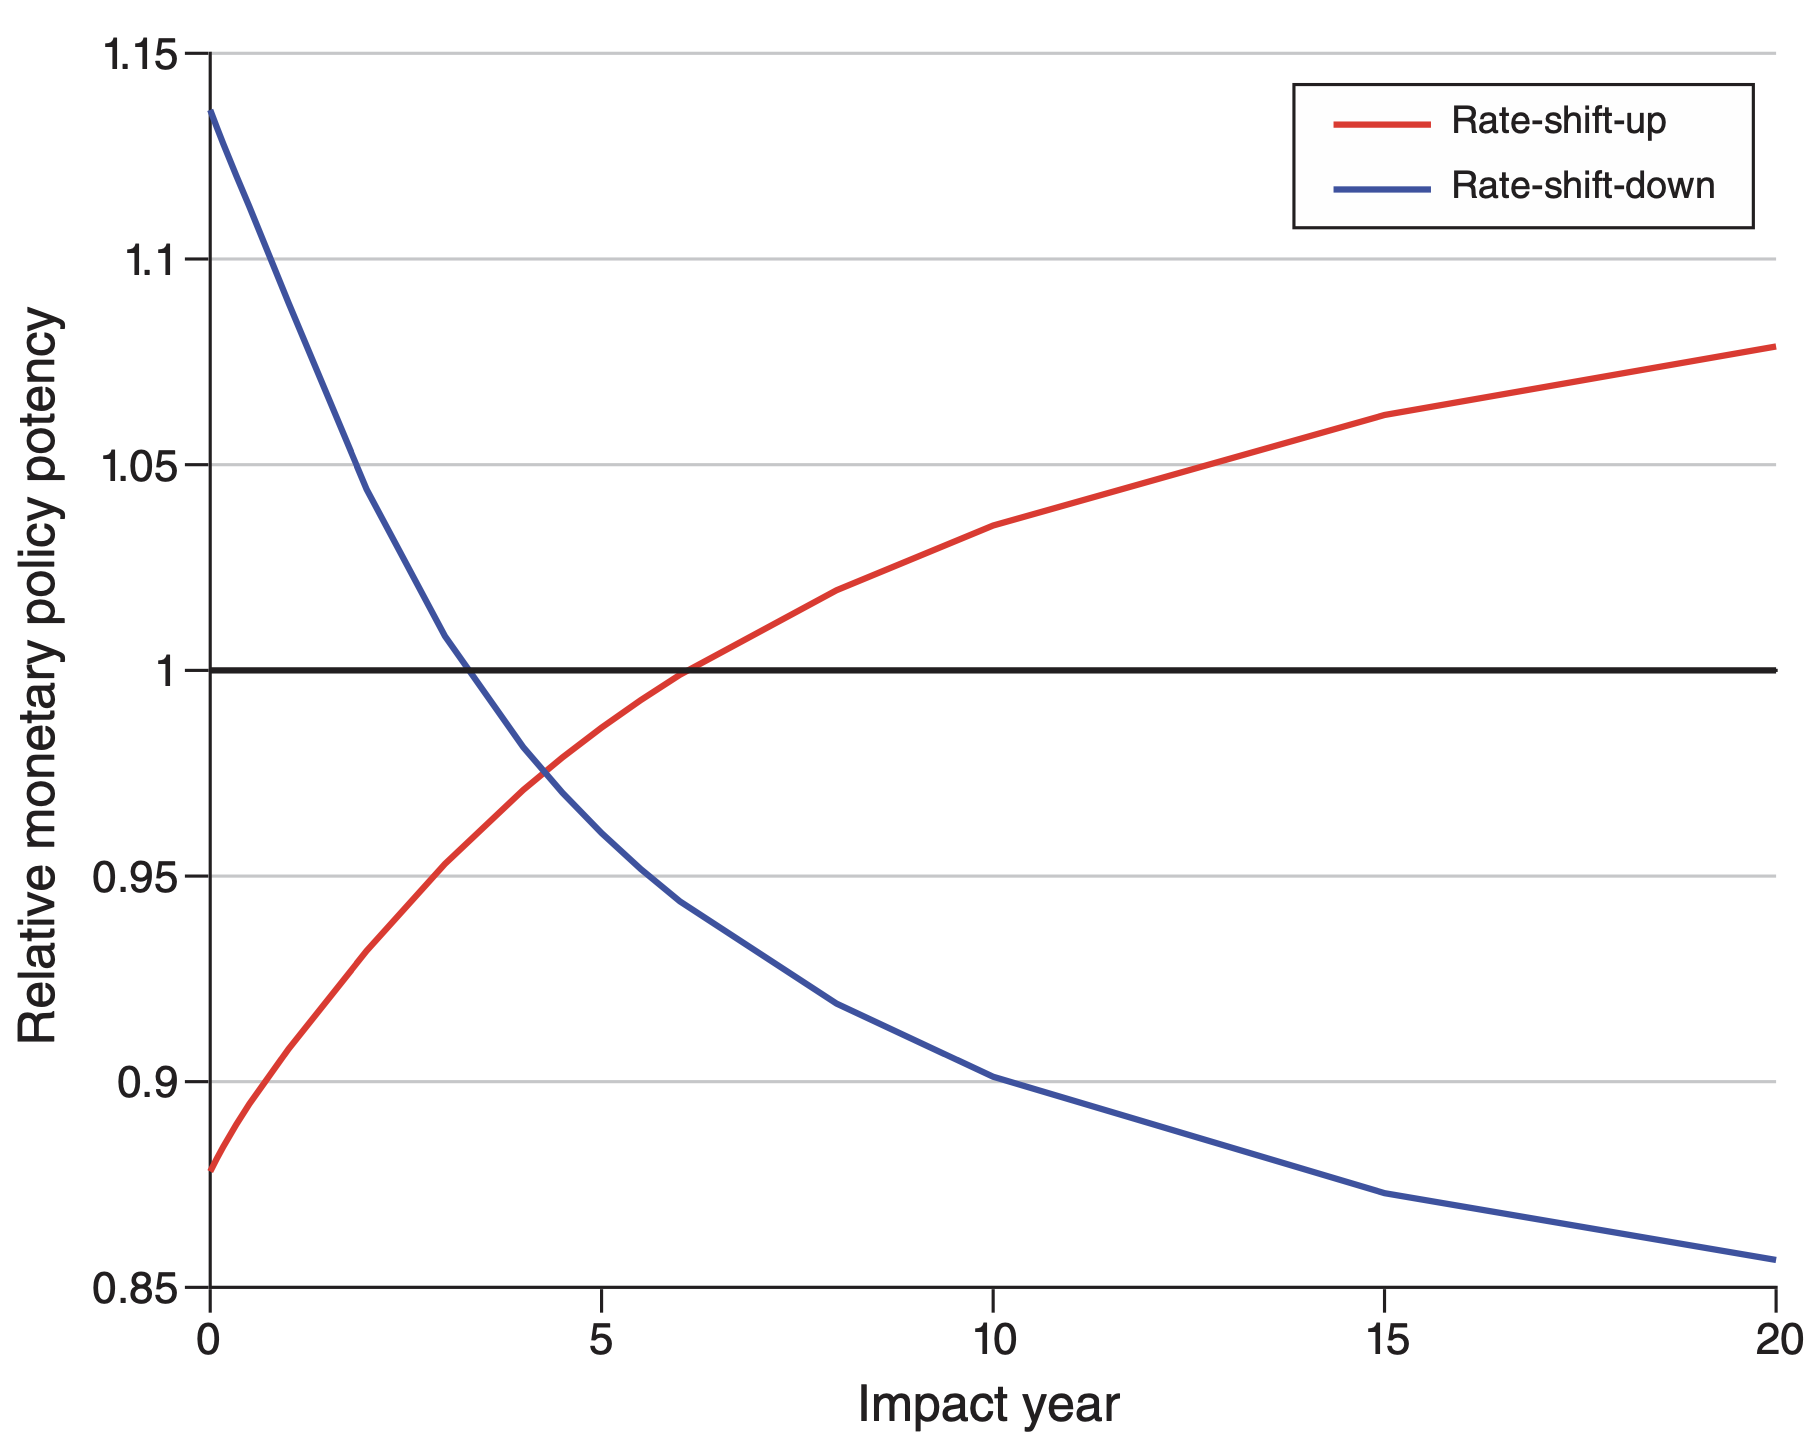
\includegraphics[scale=0.3]{figures/BMTVFIG14.png}	
    \end{center}
\end{frame}

\begin{frame}
    \frametitle{Consumption Effects}
    \begin{center}
    	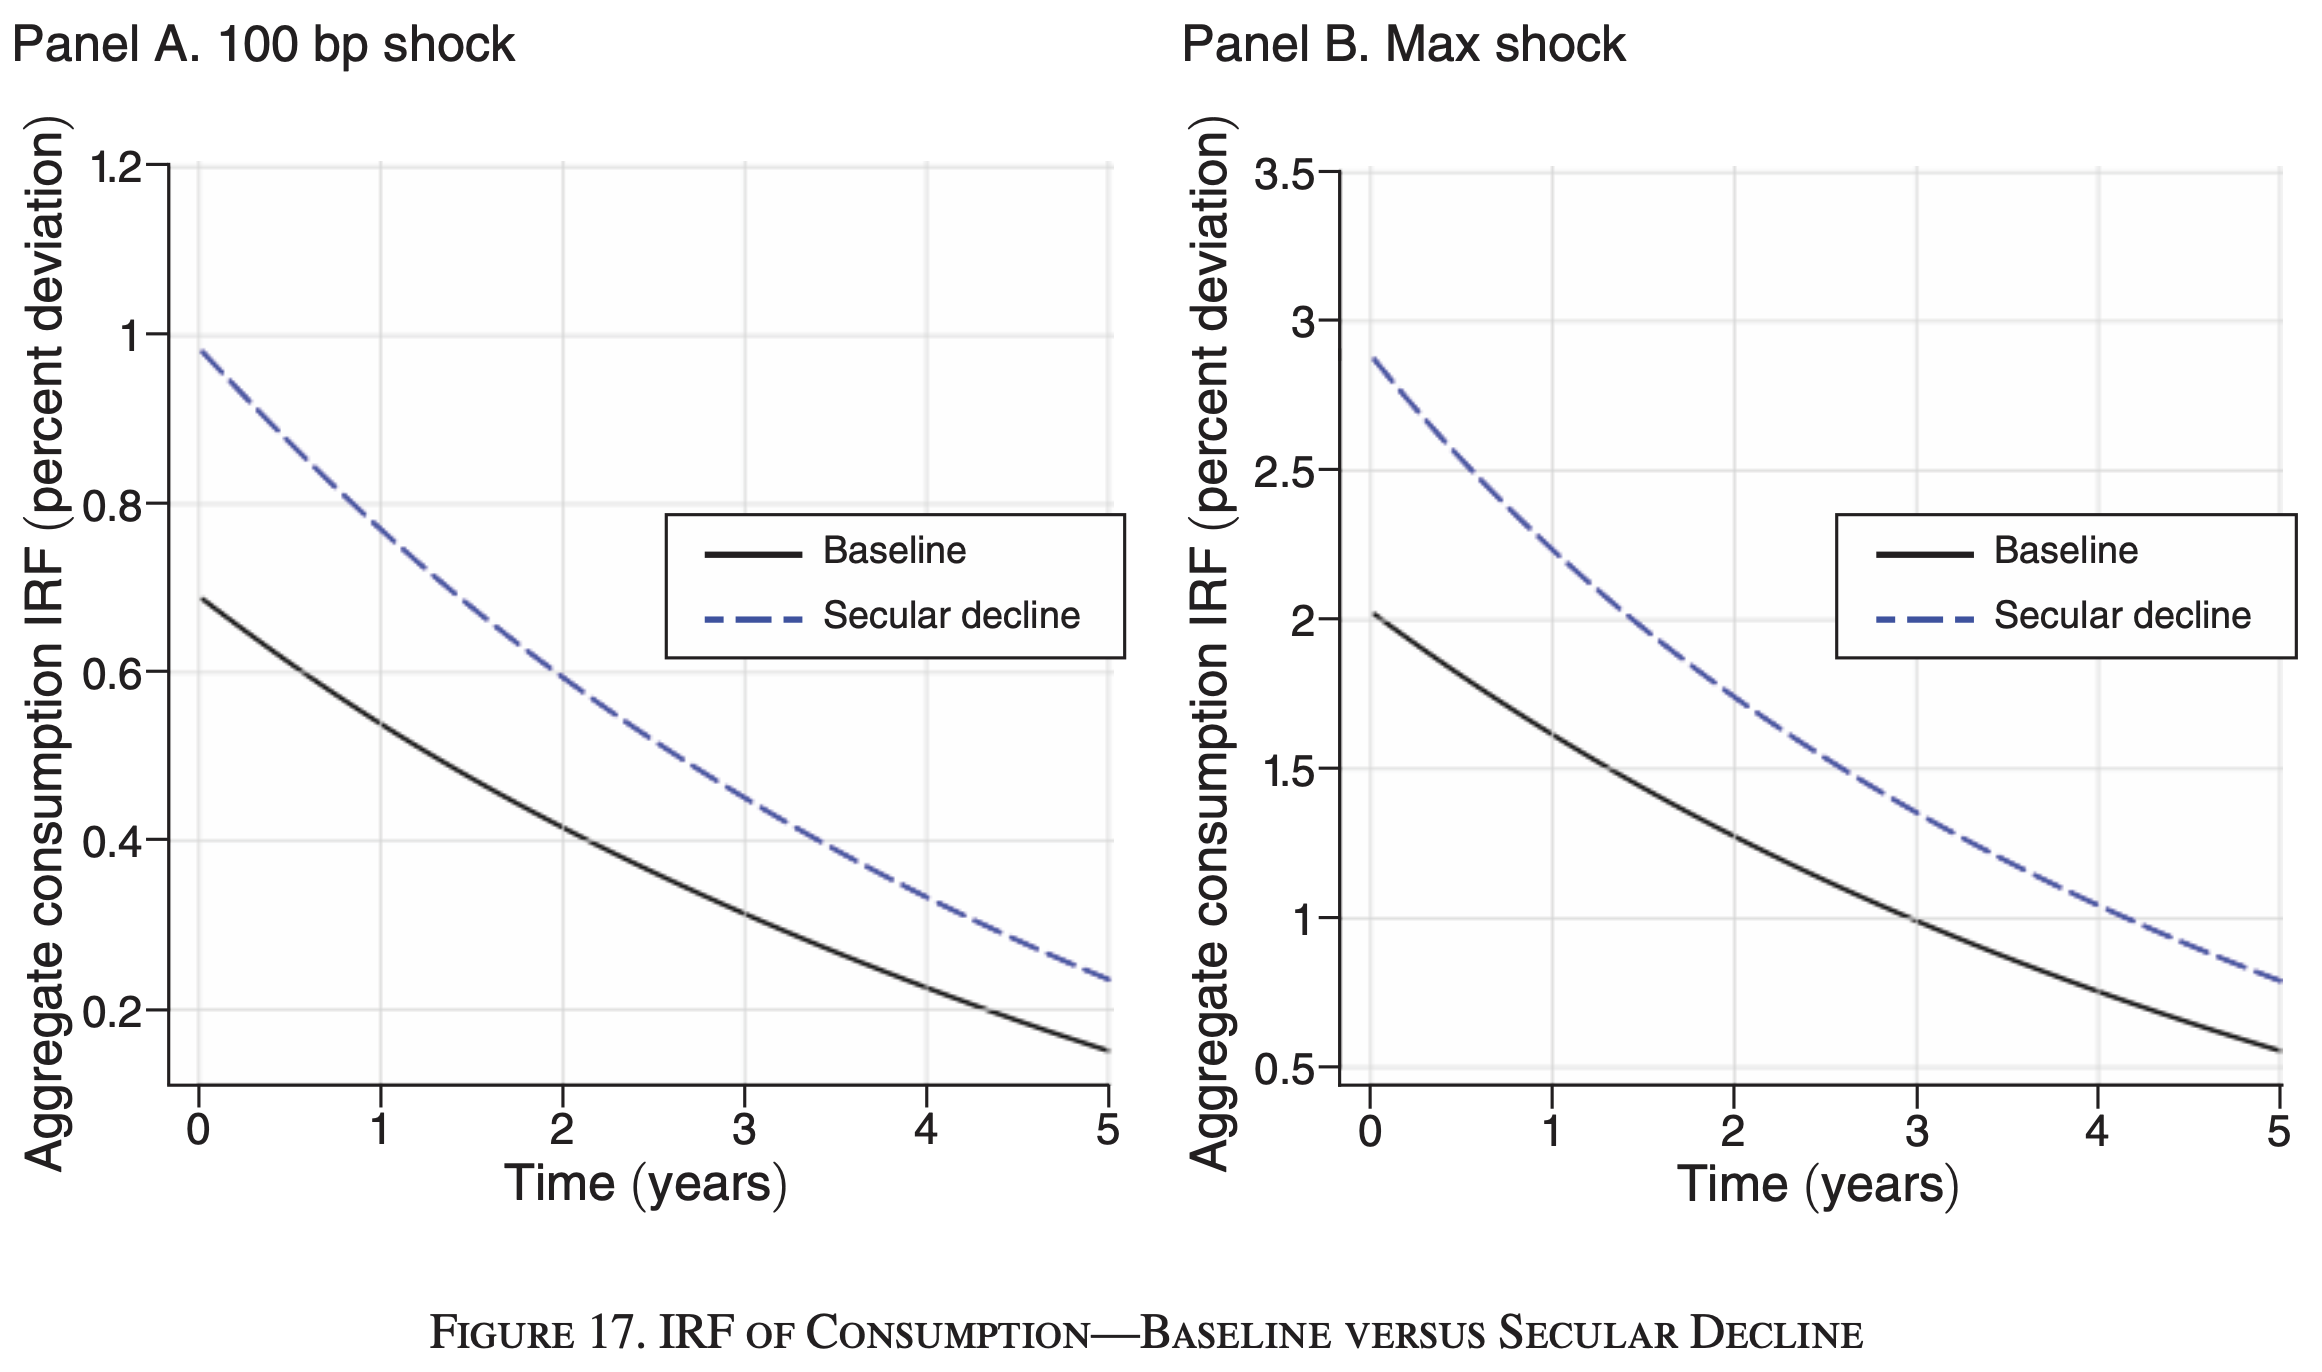
\includegraphics[scale=0.3]{figures/BMTVFIG17.png}	
    \end{center}
\end{frame}

\begin{frame}
    \frametitle{Questions}
	\begin{itemize}
		\item Convincing?
	\end{itemize}
\end{frame}


%%%%%%%%%%%%%%%%%%%%%%%%%%%%%%%%%%%%%%%%%%%%%%%%%%
\section{McKay, Wieland (2021)}
%%%%%%%%%%%%%%%%%%%%%%%%%%%%%%%%%%%%%%%%%%%%%%%%%%

\begin{frame}
    \frametitle{Does Central Bank Create or Borrow Demand?}
    \begin{itemize}
    	\item In standard NK model:
    	\begin{align*}
    		y_t  &= -\frac{1}{\sigma}r_t +  y_{t+1} \\
    		&= -\frac{1}{\sigma}\sum_{s=0}^{\infty}r_{t+s} + \lim_{T \rightarrow \infty} y_{t+1} 
    	\end{align*}
    	\item Central bank creates demand and output by changing $r_t$.
    	\item Past $r_t$ has no bearing on future AD.
    	\item[$\Rightarrow$] Central bank can create AD subject to ZLB constraint.
    	\item This paper: with durable goods, central bank is much more in the business of borrowing demand than creating demand.
    \end{itemize}
\end{frame}


\begin{frame}
\frametitle{Model: Households}
\begin{itemize}
\item Households consume non-durables and durables.
	\begin{align*}
%		\max  E_{i0}\int_{t=0}^{\infty}e^{-\rho t} \left[ u\left( c_{it}, \only<5->{\redtext{q_{it}}}\only<-4>{\phantom{q_{it}}} d_{it} \right) - v(n_{it})  \right]\dif t 
		\max  E_{i0}\int_{t=0}^{\infty}e^{-\rho t}   u\left( c_{it}, q_{it} d_{it} \right)  d t 
	\end{align*}
\item Durables subject to:
	\begin{itemize}
	\item fixed adjustment cost (if adjust) $a_{it}'+p_t d_{it}' = a_{it}+(1-f)p_t d_{it}$
	\item depreciation and maintenance cost $dt d_{it} = -(1-\chi)\delta d_{it} $
	\item operating cost (e.g. household utilities, gas, taxes) $\nu  d_{it}$
	\item match-quality shocks $q_{it} =1$, drops to zero with intensity $\theta$
	\end{itemize}
\item Idiosyncratic labor income risk\\ $y_{it} = \left(1-\tau_t\right) Y_t z_{it}$\hspace{2cm}
$d \ln z_{it} = -\rho_z \ln z_{it} + \sigma_z d \mathcal W_{it} $
\item Save in liquid assets
         $dt a_{it} = r_t a_{it} + r_t^b a_{it}I_{\{a_{it}<0\}} - c_{it} +  y_{it}-(\chi\delta p_t + \nu)  d_{it}$ 
\item Collateralized borrowing $a_{it} \ge -\lambda(1-f)p_{t} d_{it}$
\item Sticky information (Carrol et al, 2018; Auclert et al, 2020).
\end{itemize}
\end{frame}

\begin{frame}
    \frametitle{Hazard Rate}
    \begin{center}
    	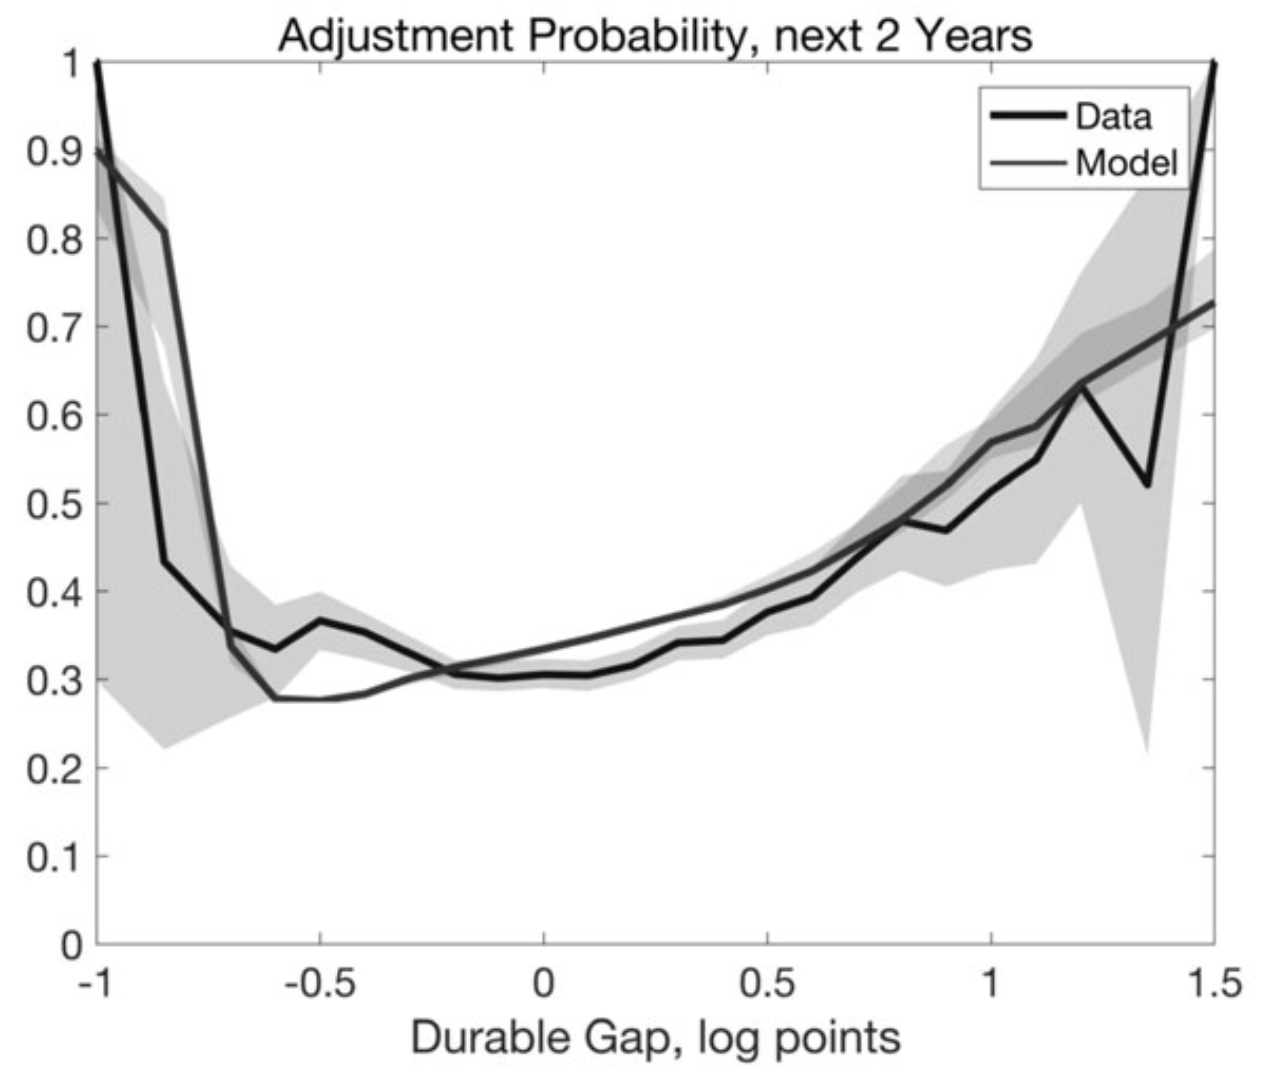
\includegraphics[scale=0.3]{figures/MWFIG1.png}	
    \end{center}
\end{frame}

\begin{frame}
    \frametitle{Intertemporal Shifting in the Data}
    \begin{center}
    	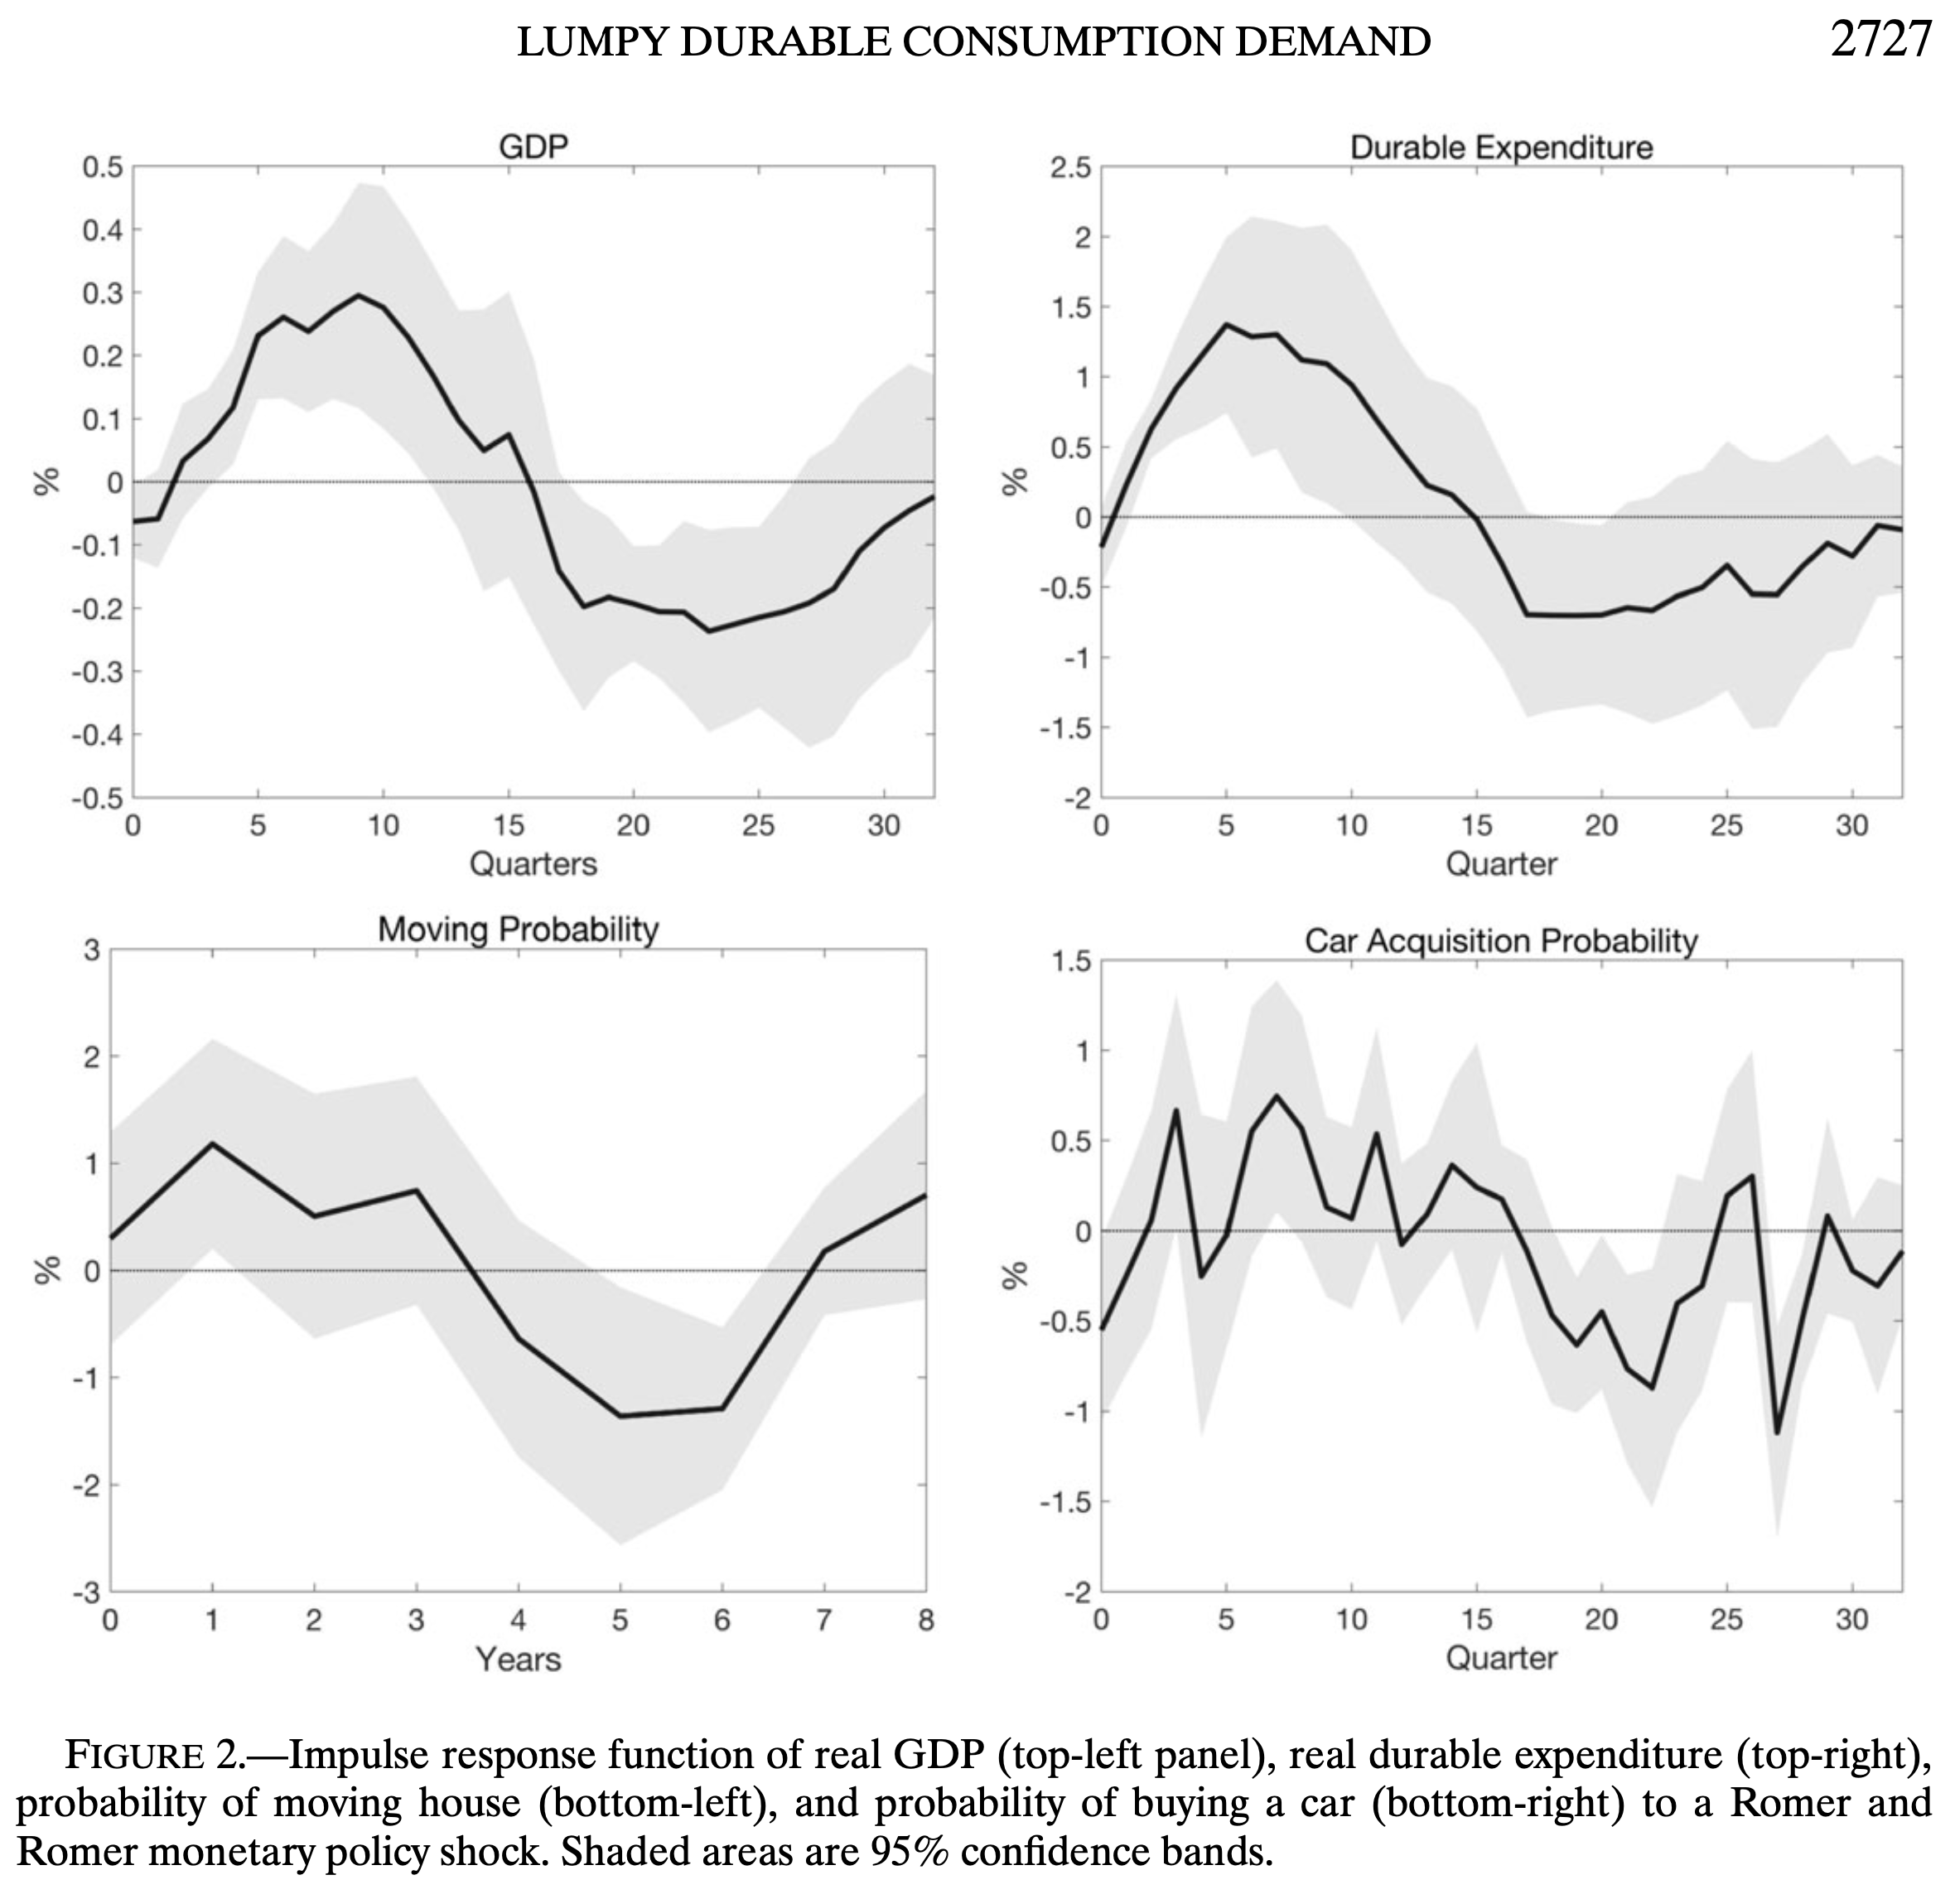
\includegraphics[scale=0.2]{figures/MWFIG2.png}	
    \end{center}
\end{frame}

\begin{frame}
    \frametitle{Intertemporal Shifting in the Data}
    \begin{center}
    	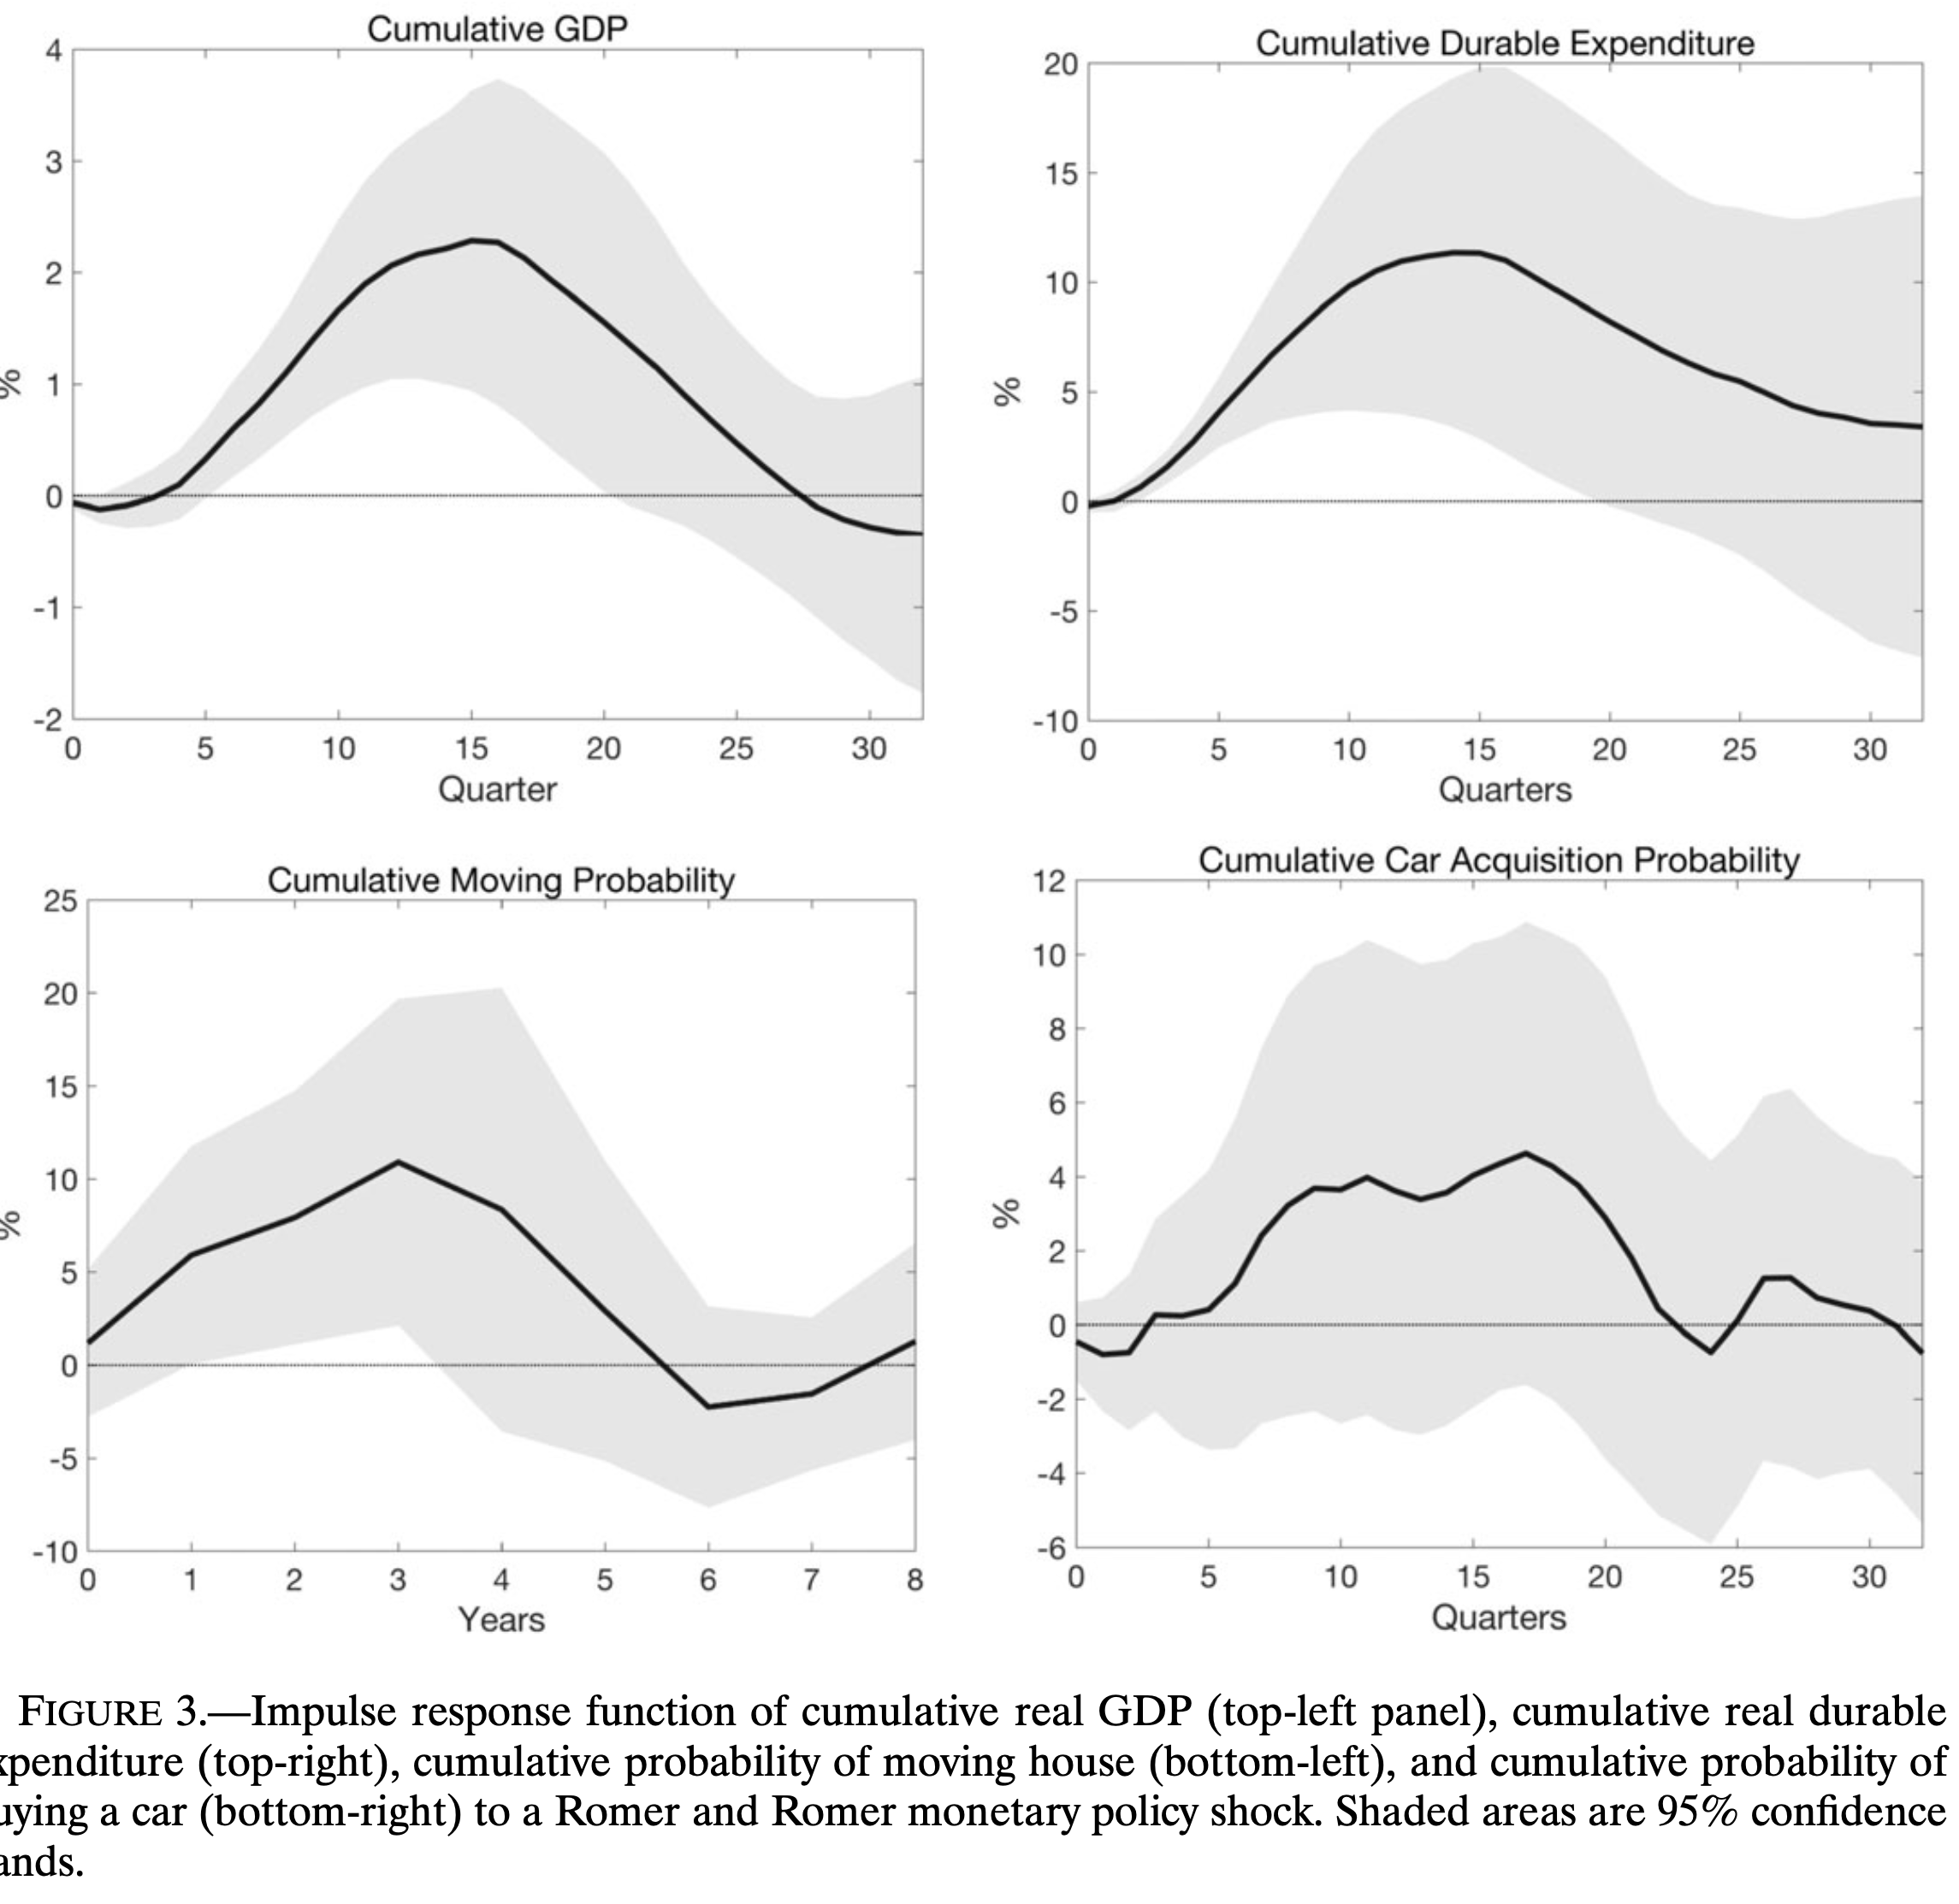
\includegraphics[scale=0.2]{figures/MWFIG3.png}	
    \end{center}
\end{frame}

\begin{frame}
    \frametitle{Model vs Data}
    \begin{center}
    	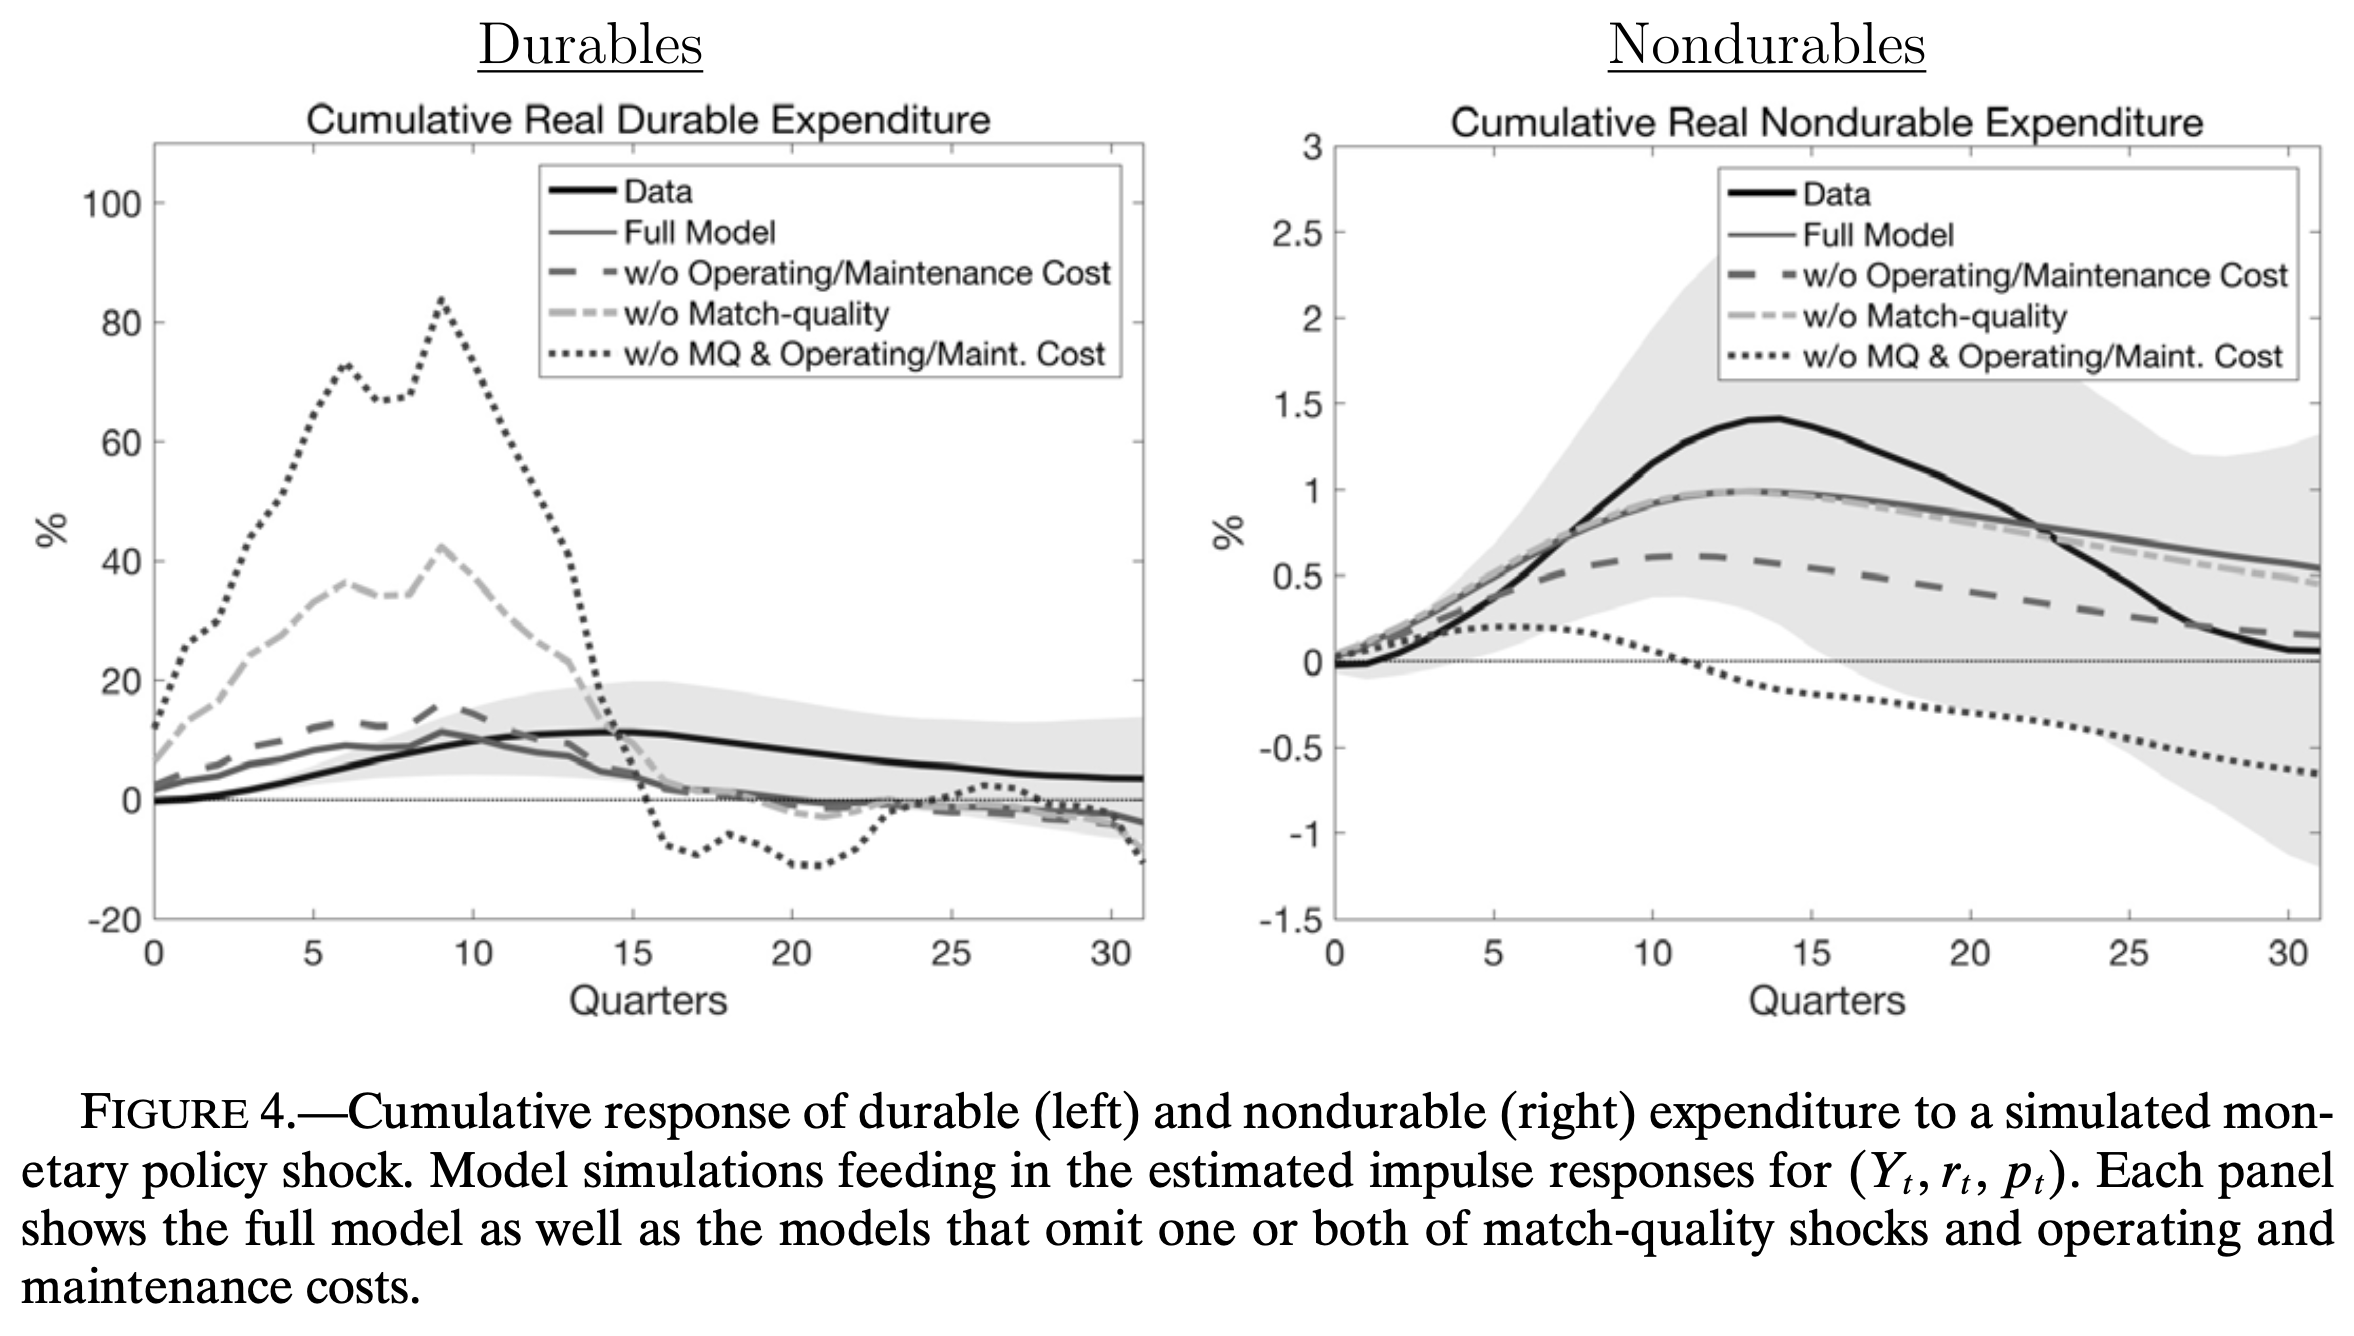
\includegraphics[scale=0.3]{figures/MWFIG4.png}	
    \end{center}
\end{frame}

\begin{frame}
    \frametitle{Model vs Data}
    \begin{center}
    	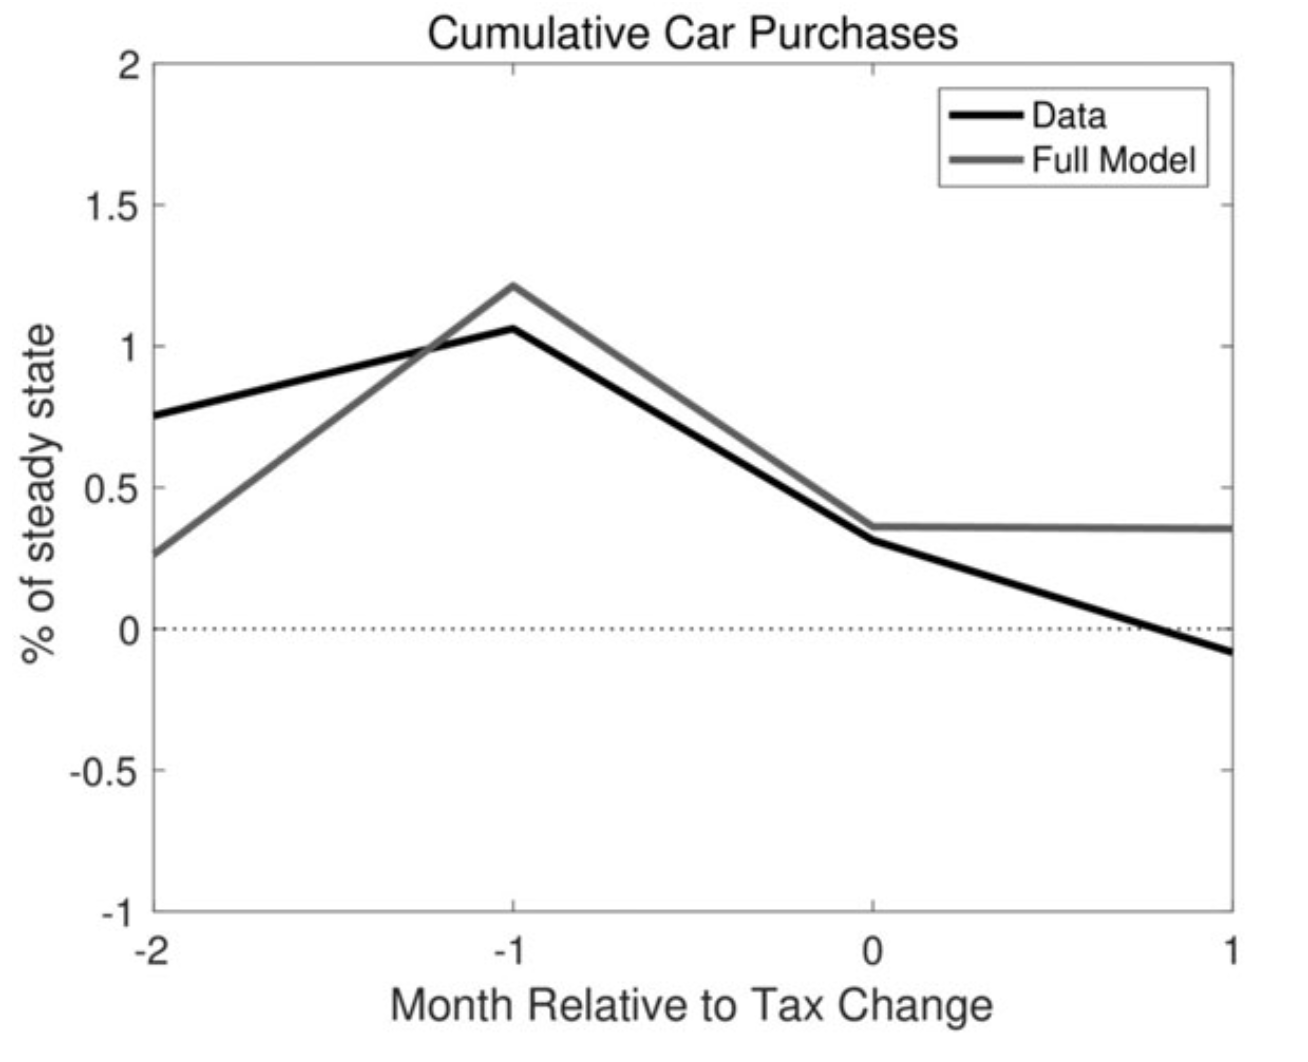
\includegraphics[scale=0.3]{figures/MWFIG6.png}	
    \end{center}
\end{frame}


\begin{frame}\frametitle{The Monetary Transmission Matrix}
\begin{itemize}
\item Solve model with sequence space methods. 
\item The ``monetary transmission matrix'':
\begin{align*}
  \mathcal{M} =\begin{pmatrix}
    \frac{d \hat{Y}_0}{d r_0} & \frac{d \hat{Y}_0}{d r_{1}} & \frac{d \hat{Y}_0}{d r_{2}} & \hdots \\
    \frac{d \hat{Y}_{1}}{d r_0} & \frac{d \hat{Y}_1}{d r_{1}} & \frac{d \hat{Y}_1}{d r_{2}} & \hdots \\
    \frac{d \hat{Y}_{2}}{d r_0} & \frac{d \hat{Y}_2}{d r_{1}} & \frac{d \hat{Y}_2}{d r_{2}} & \hdots \\
    \vdots & \vdots & \vdots & \ddots 
  \end{pmatrix}
\end{align*}
\item GE effect of monetary news on output gap.\\
\begin{itemize}
	\item Below-diagonal elements capture intertemporal-shifting effects.
	\item Above-diagonal elements capture forward guidance effects.
\end{itemize}
\end{itemize}
\end{frame}

\begin{frame}
    \frametitle{IRF to $r_0$ and News}
    \begin{center}
    	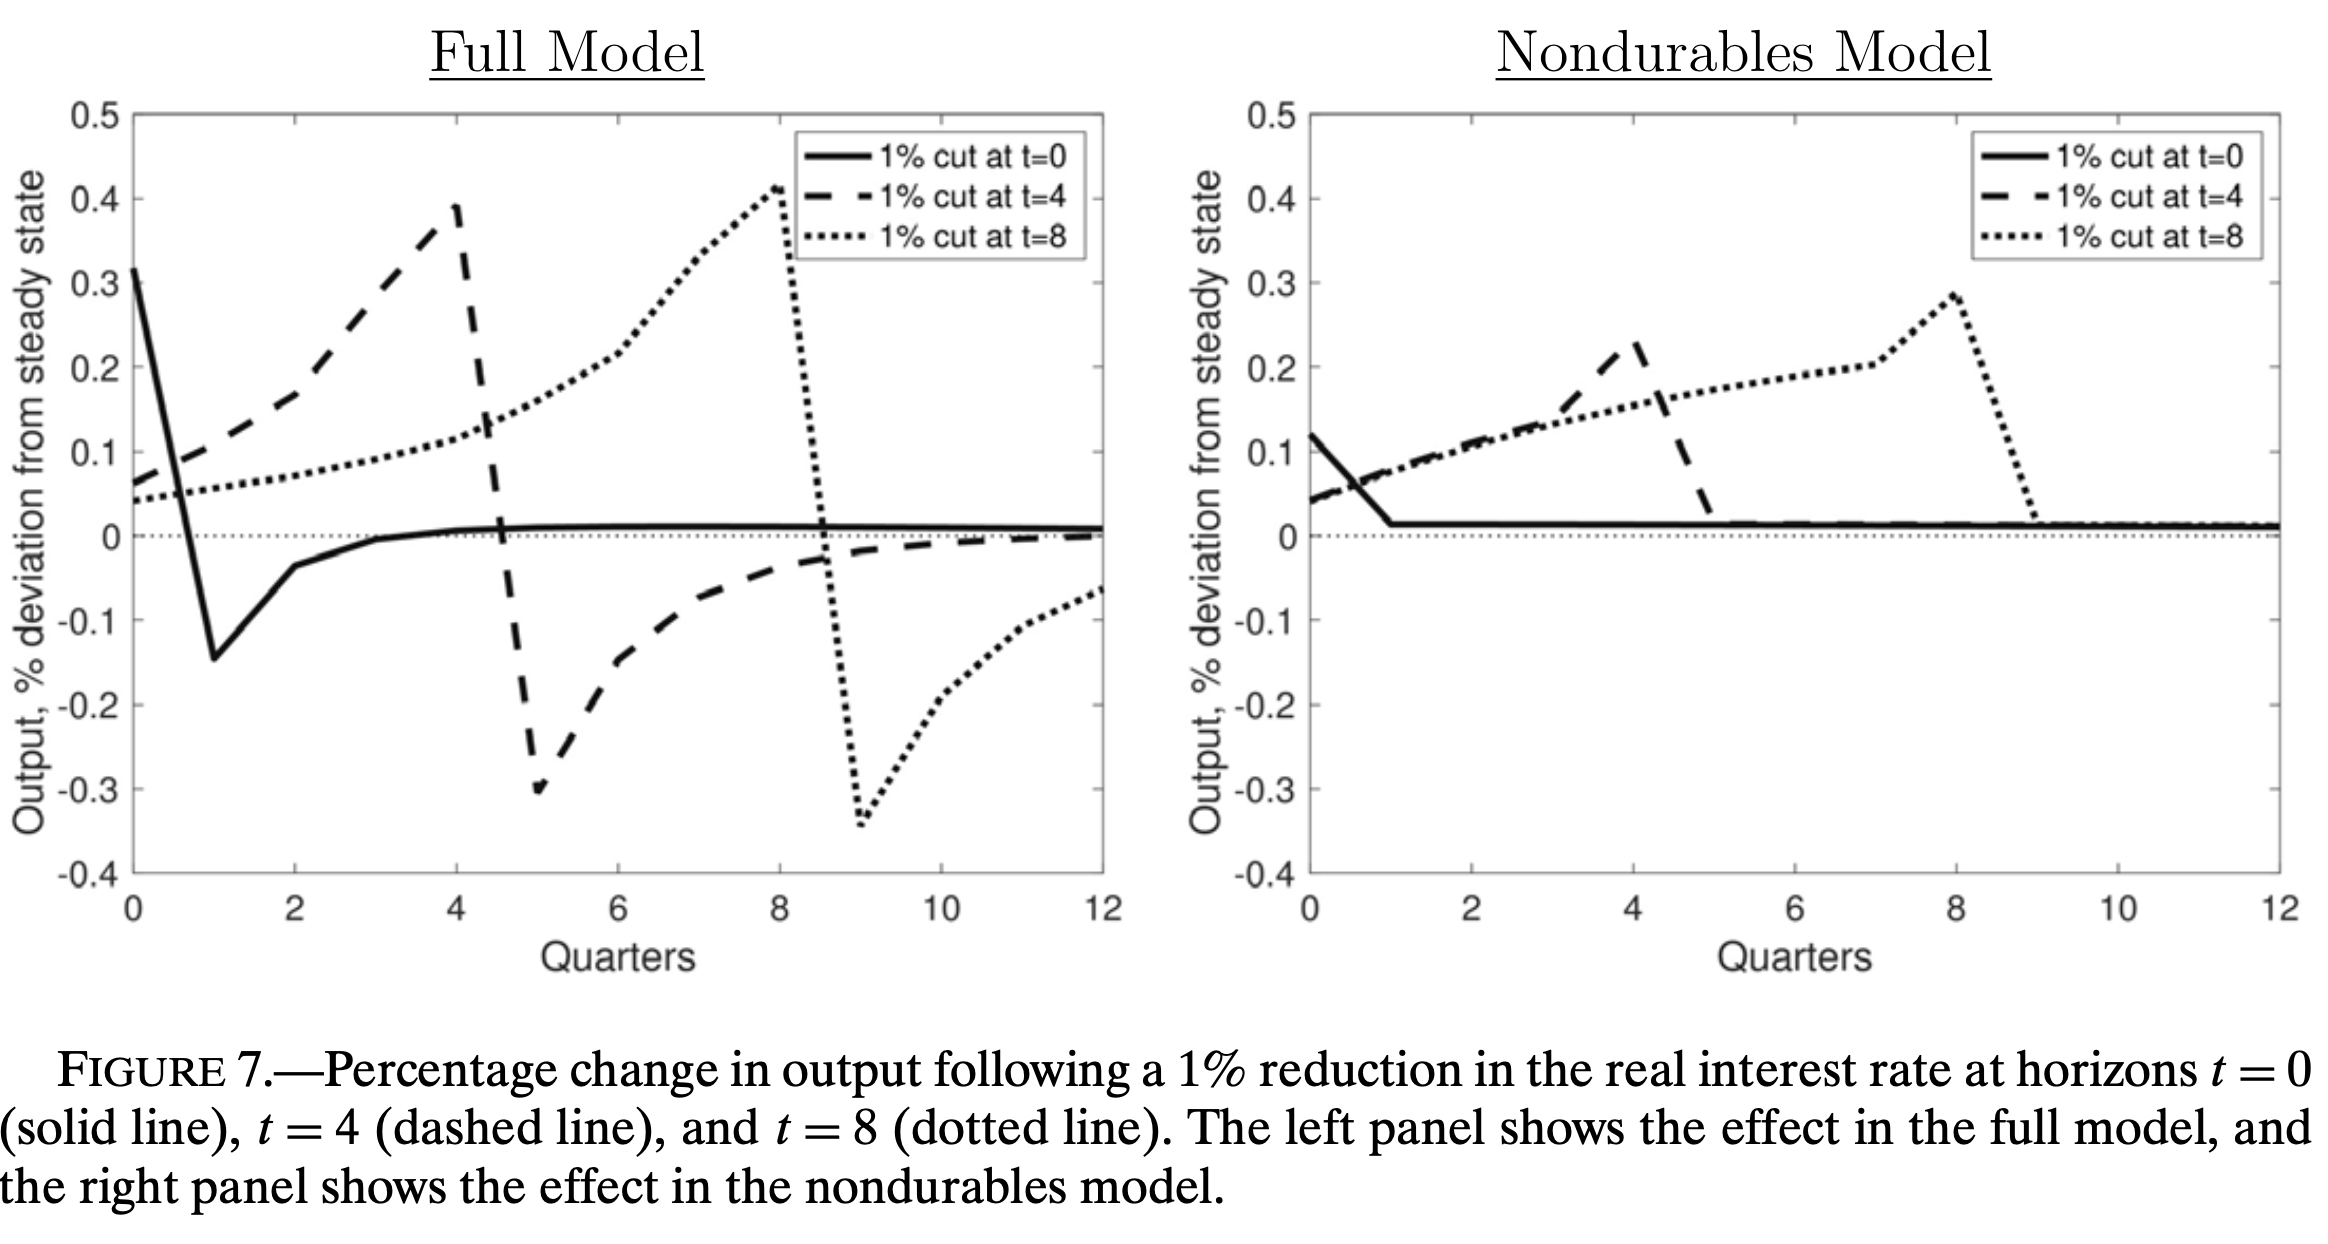
\includegraphics[scale=0.3]{figures/MWFIG7.png}	
    \end{center}
\end{frame}

\begin{frame}\frametitle{Great Recession--Filtering the Data}
\begin{itemize}
\item Construct IRFs for shocks to $Z_t,G_t,r^b_t,\eta_t$. \vfill
\item Match time series:
	\begin{itemize}
	\item output gap, 
	\item durable spending,
	\item real interest rate,
	\item mortgage-treasury spread.
	\end{itemize} \vfill
\item Unique sequence of shocks that fit data exactly given initial condition. (Kalman filter with no observational error.)
\begin{itemize}
	\item No need for state transition matrix.\vfill
	\end{itemize}
\item Account for zero lower bound using monetary news shocks.
\end{itemize}
\end{frame}

\begin{frame}
   \frametitle{Model predicts slow normalization of real rate}
    \begin{center}
    	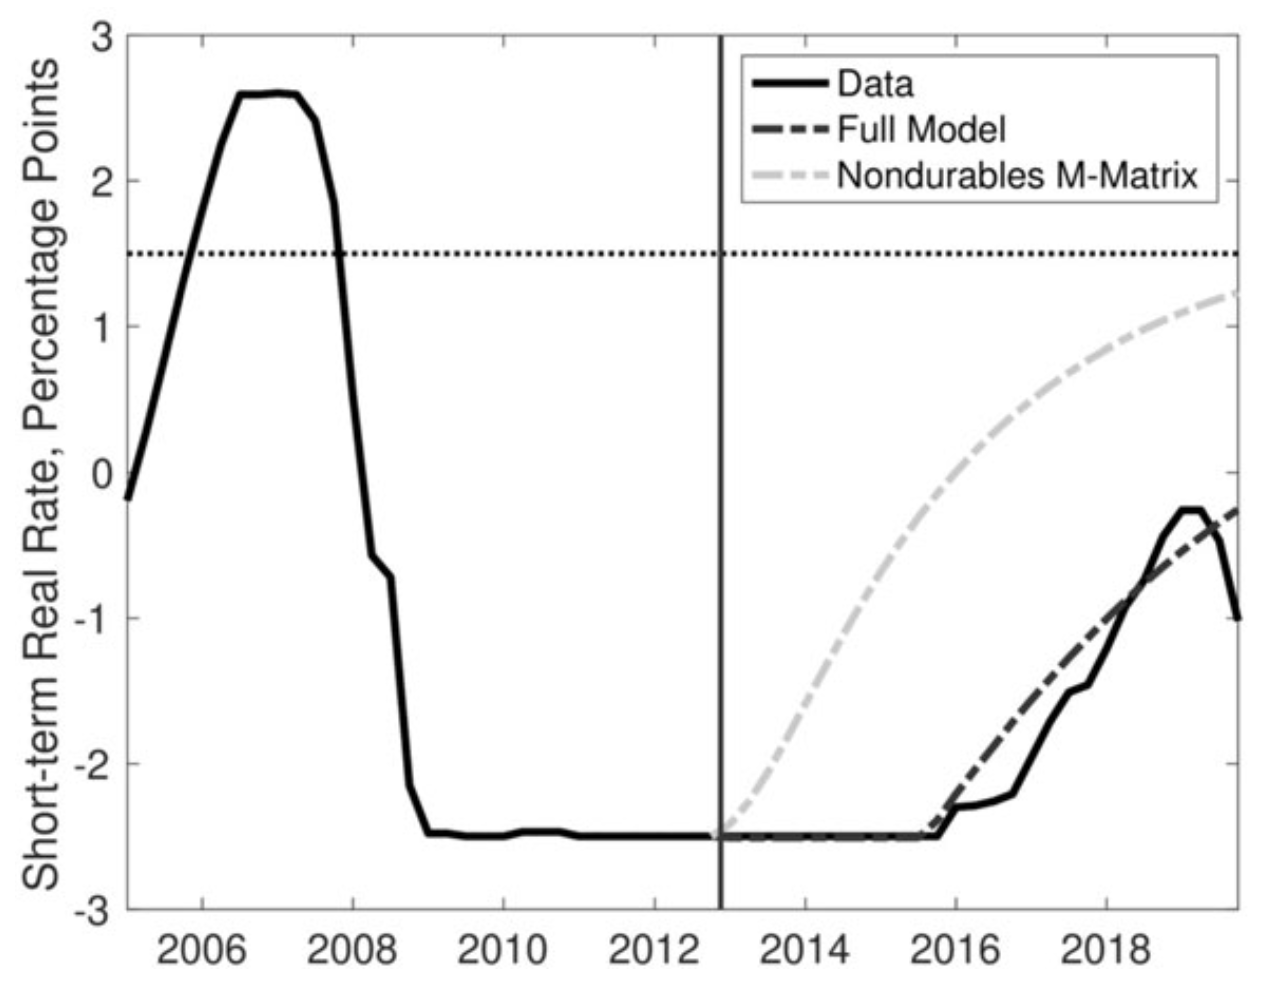
\includegraphics[scale=0.3]{figures/MWFIG9.png}	
    \end{center}
\end{frame}

\begin{frame}
    \frametitle{Contribution of Intertemporal Shifting to $r^*$}
    \begin{center}
    	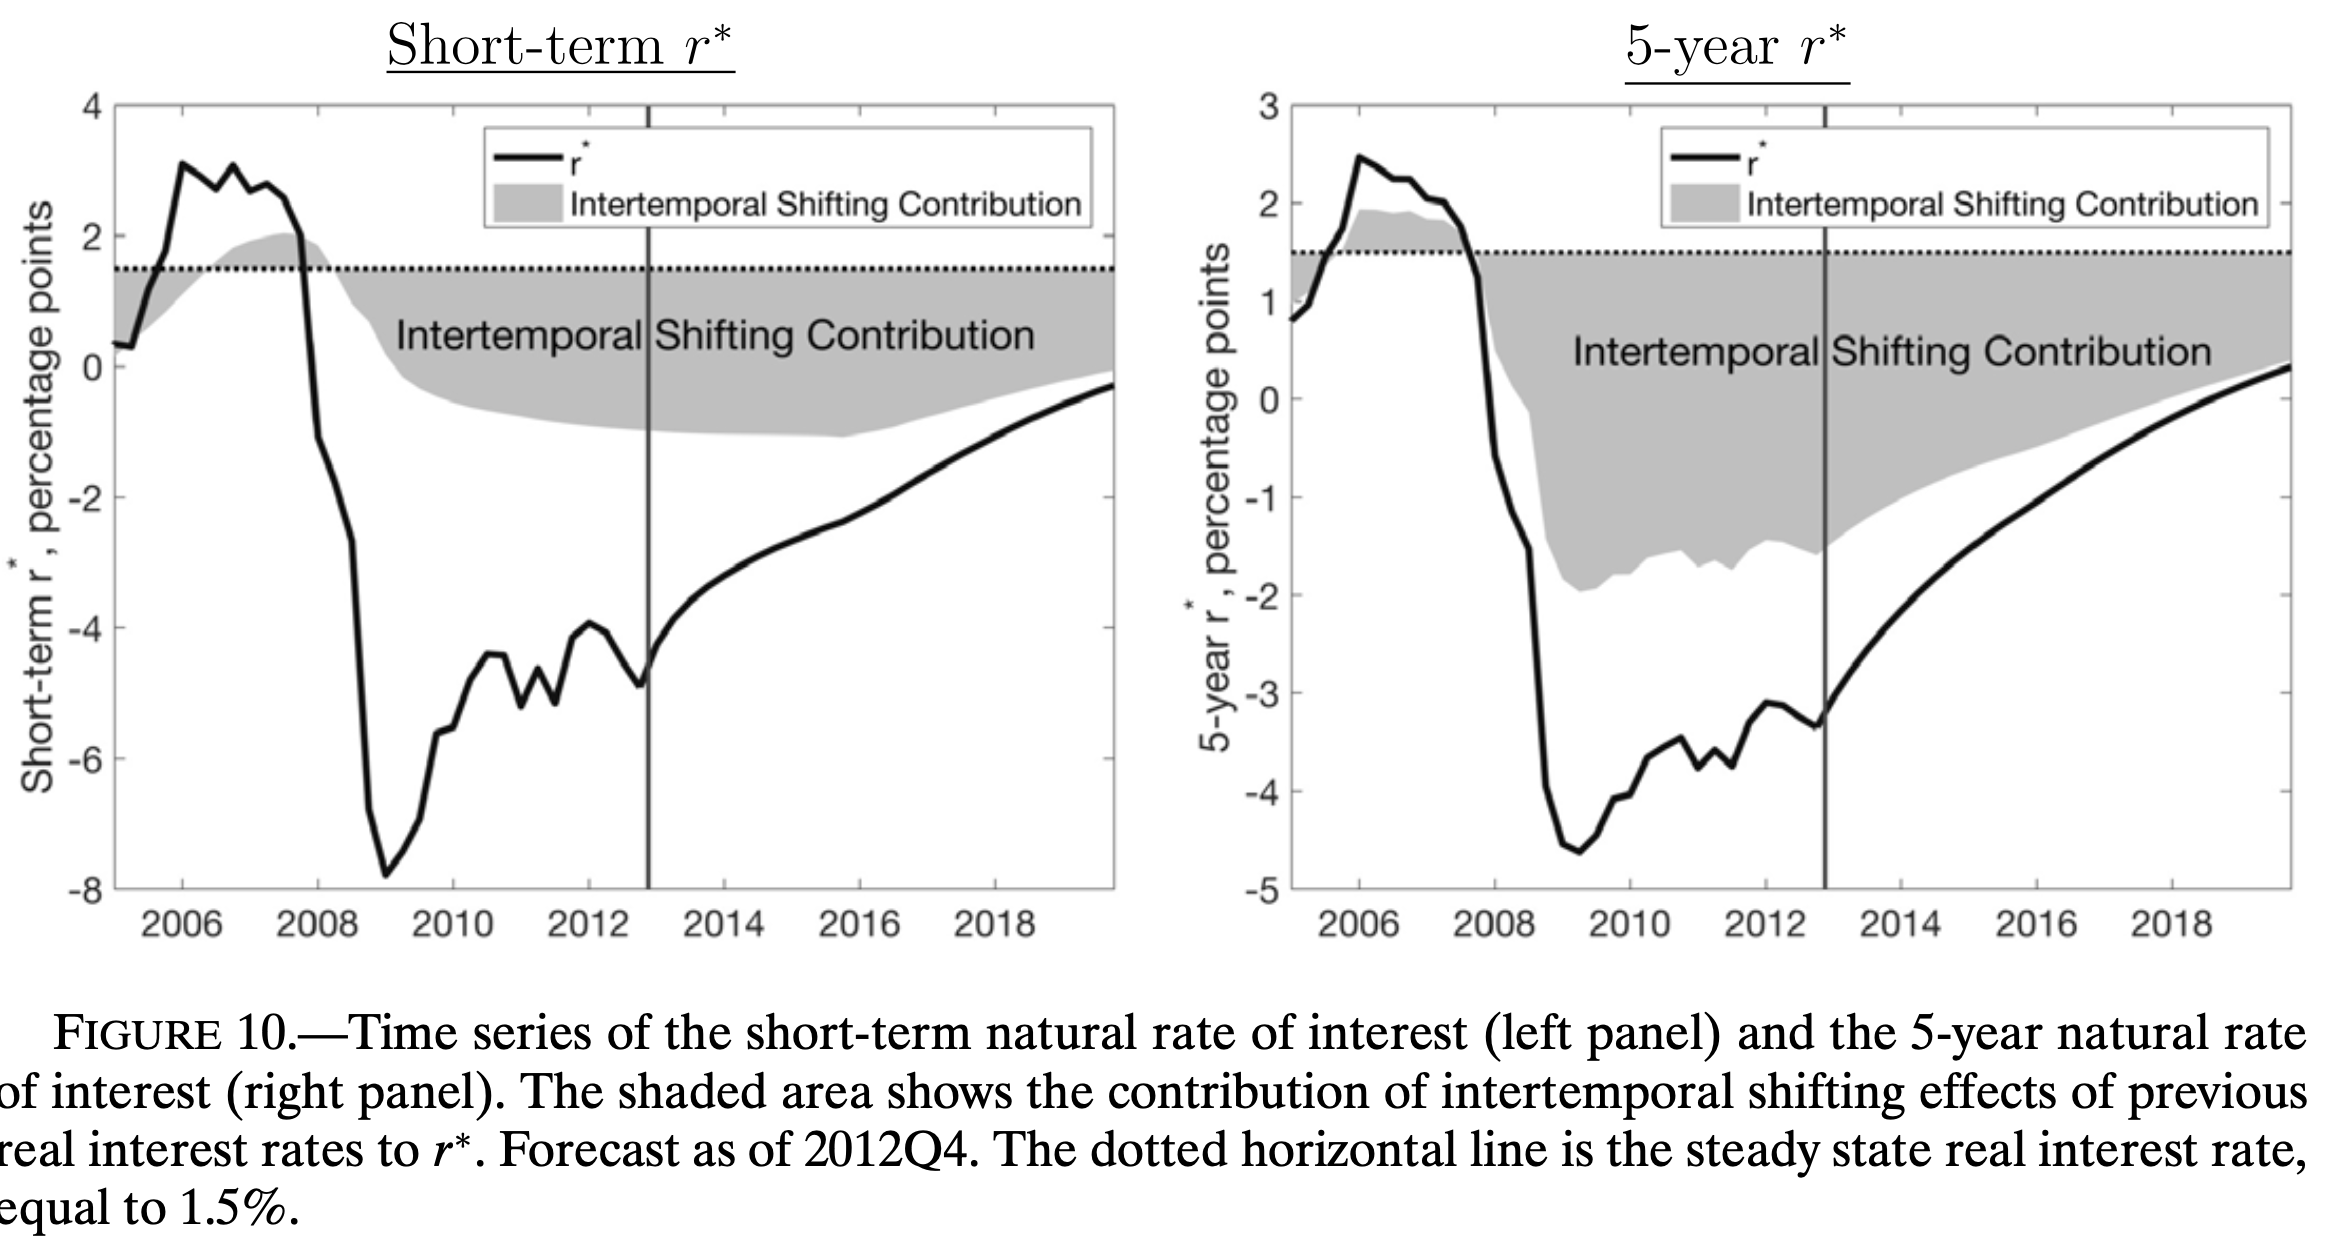
\includegraphics[scale=0.3]{figures/MWFIG10.png}	
    \end{center}
\end{frame}

\begin{frame}
    \frametitle{Contribution Shocks to $r^*$}
    \begin{center}
    	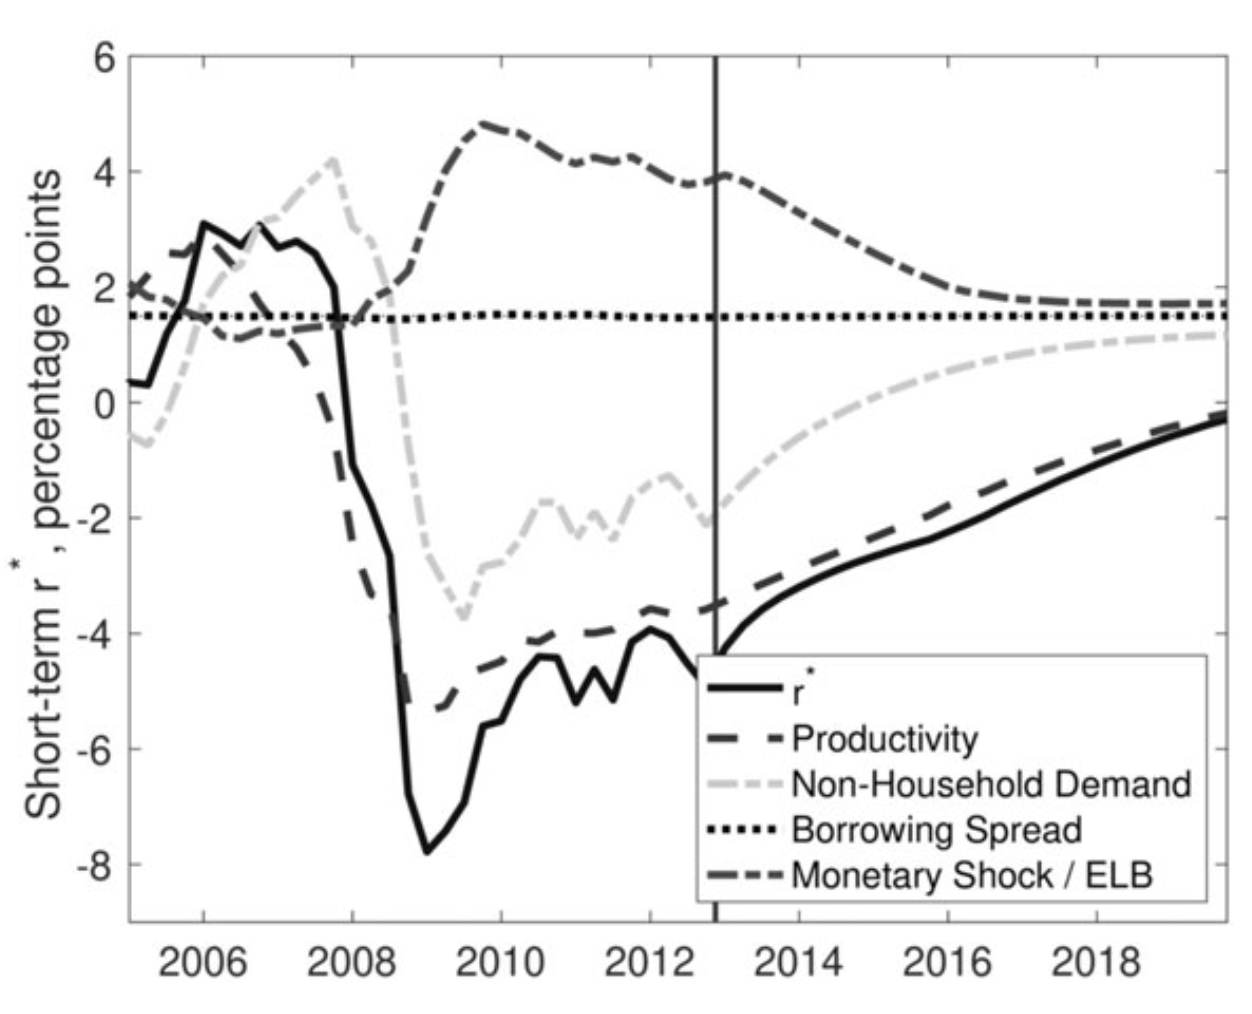
\includegraphics[scale=0.3]{figures/MWFIG11.png}	
    \end{center}
\end{frame}

\begin{frame}
    \frametitle{Questions}
	\begin{itemize}
		\item Convincing?
		\item What role does the micro evidence play?
	\end{itemize}
\end{frame}

%%%%%%%%%%%%%%%%%%%%%%%%%%%%%%%%%%%%%%%%%%%%%%%%%%
\section{McKay, Wieland (2022)}
%%%%%%%%%%%%%%%%%%%%%%%%%%%%%%%%%%%%%%%%%%%%%%%%%%

\begin{frame}
    \frametitle{Forward Guidance Puzzle}
    \begin{itemize}
    	\item In standard NK model:
    	\begin{align*}
    		y_t  &= -\frac{1}{\sigma}r_t +  y_{t+1} \\
    		&= -\frac{1}{\sigma}\sum_{s=0}^{\infty}r_{t+s} + \lim_{T \rightarrow \infty} y_{t+1} 
    	\end{align*}
    	\item Credible future real rate change has the same effect on current output regardless of how distant it is.
    \end{itemize}
\end{frame}

\begin{frame}
    \frametitle{With Durable Goods}
    \begin{itemize}
    	\item MRS between durable and nondurable good is equal to user cost:
    	\begin{align*}
    		\left(\frac{\psi}{1-\psi}\frac{c_{it}}{d_{it}}\right)^{\frac{1}{\xi}} = p_t(r_t + \nu +\delta) - \dot{p}_t \equiv r_t^d
    	\end{align*}
    	\item Special role for contemporaneous real rate in durable goods demand.
    \end{itemize}
\end{frame}

\begin{frame}
    \frametitle{Frictionless Durable Model}
    \begin{center}
    	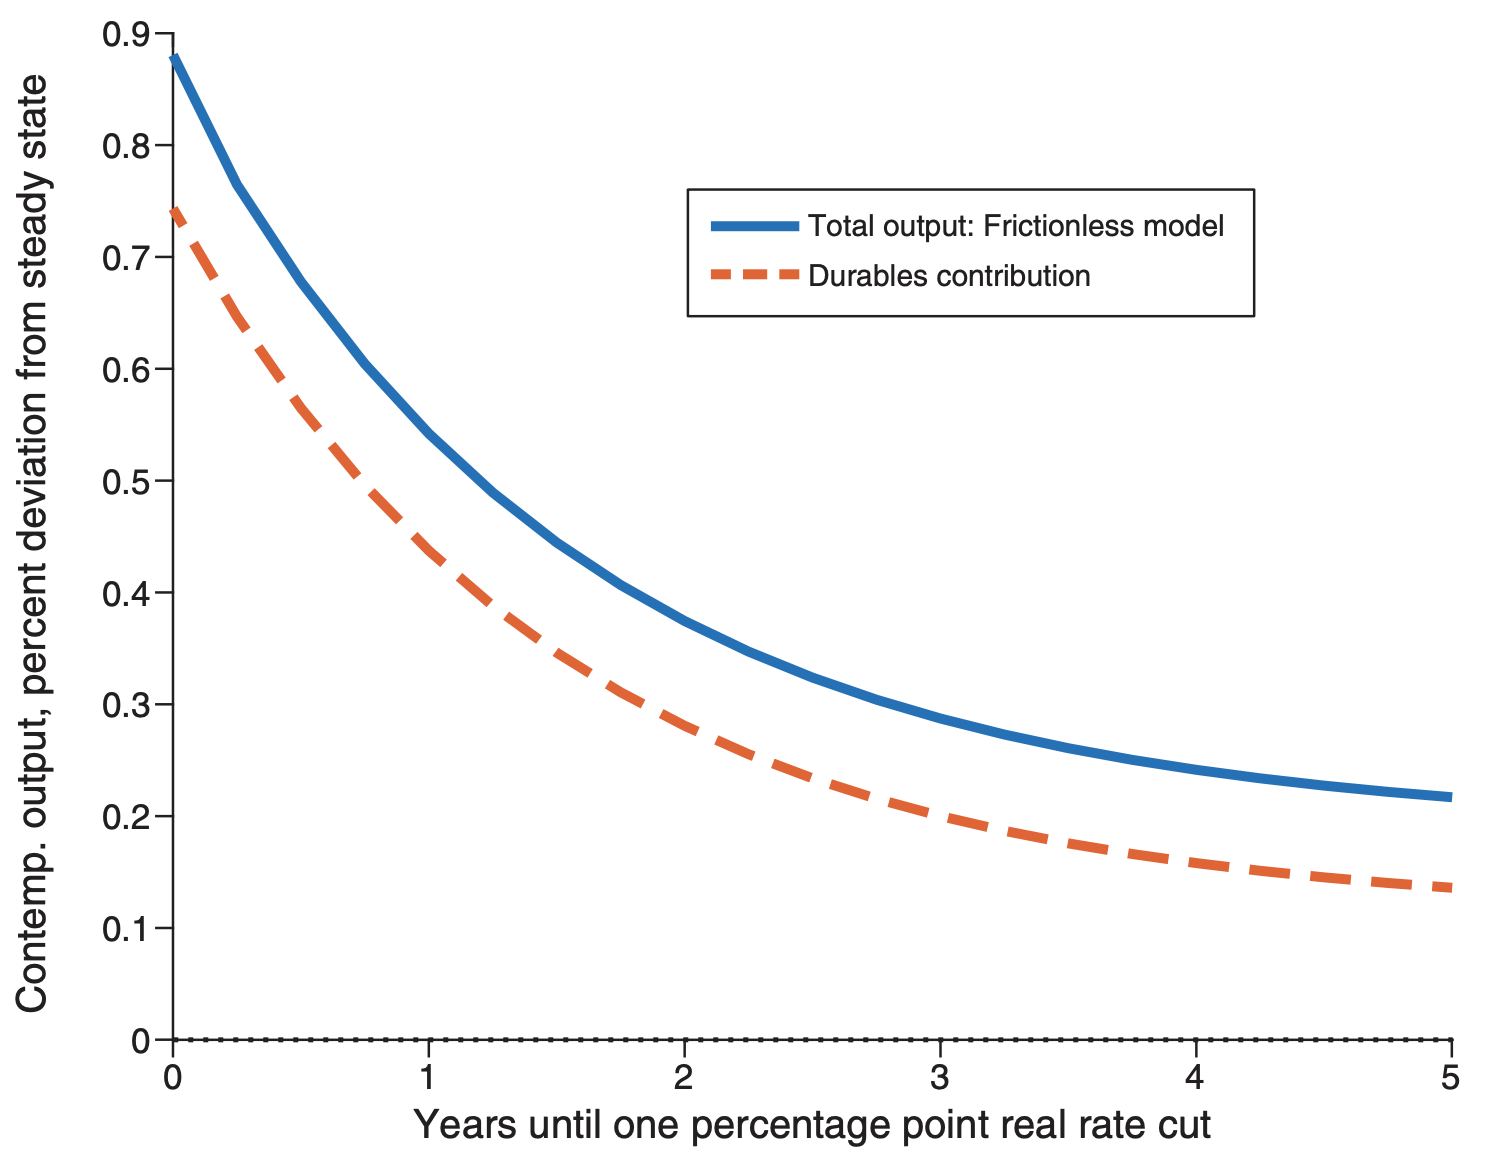
\includegraphics[scale=0.3]{figures/MWFGFIG1.png}	
    \end{center}
\end{frame}


\begin{frame}
    \frametitle{Lumpy durables}
    \begin{itemize}
    	\item Frictionless model inconsistent with lumpy nature of durable adjustment. 
    	\item[$\Rightarrow$] How credible are the results?
    \end{itemize}
\end{frame}

\begin{frame}
    \frametitle{Fixed Cost Durable Model}
    \begin{center}
    	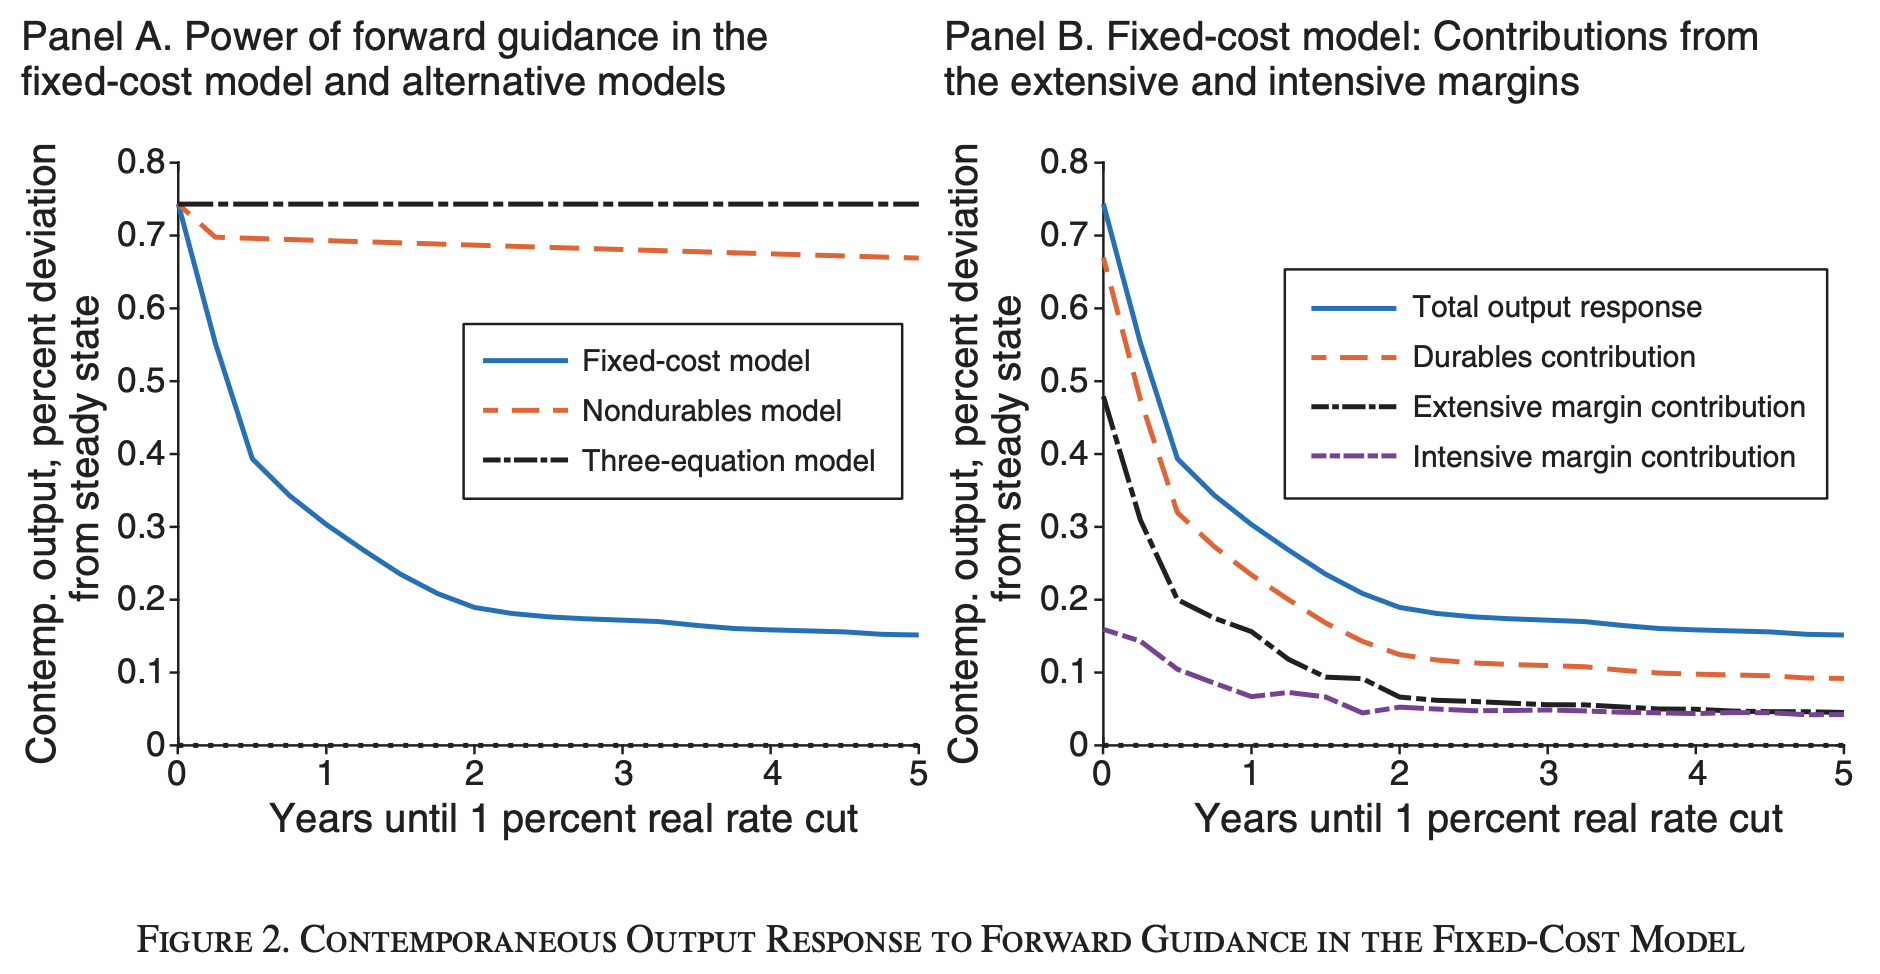
\includegraphics[scale=0.3]{figures/MWFGFIG2.png}	
    \end{center}
\end{frame}

\begin{frame}
    \frametitle{Extensive Margin}
    \begin{align*}
&\frac{u(c_t^*,d_t^*)- u(c_t,d)}{V_{a,t}(a_t^*,d_t^*,z)}= 
     r_t^d \left(d_t^*-d\right)
	+ \left[r_t^d - (\nu + \delta \chi)p_t \right]fd +  (c_t^* - c_t)  \\
	&\quad + \frac{\frac{V_{d,t}(a_t^*,d_t^*,z)}{p_t V_{a,t}(a_t^*,d_t^*,z)}-1}{1-\lambda(1-f)} \left\{\frac{a}{p_t}\left[r_t^d - (\nu + \delta \chi)p_t \right] +z (1-\tau_t)Y_t - c_t - (\nu + \delta \chi)p_t d\right\}\\
\end{align*}
\begin{itemize}
	\item Intuition: adjust now vs a little bit later.
\end{itemize}
\end{frame}

\begin{frame}
    \frametitle{Importance of Contemporaneous User Cost}
    \begin{center}
    	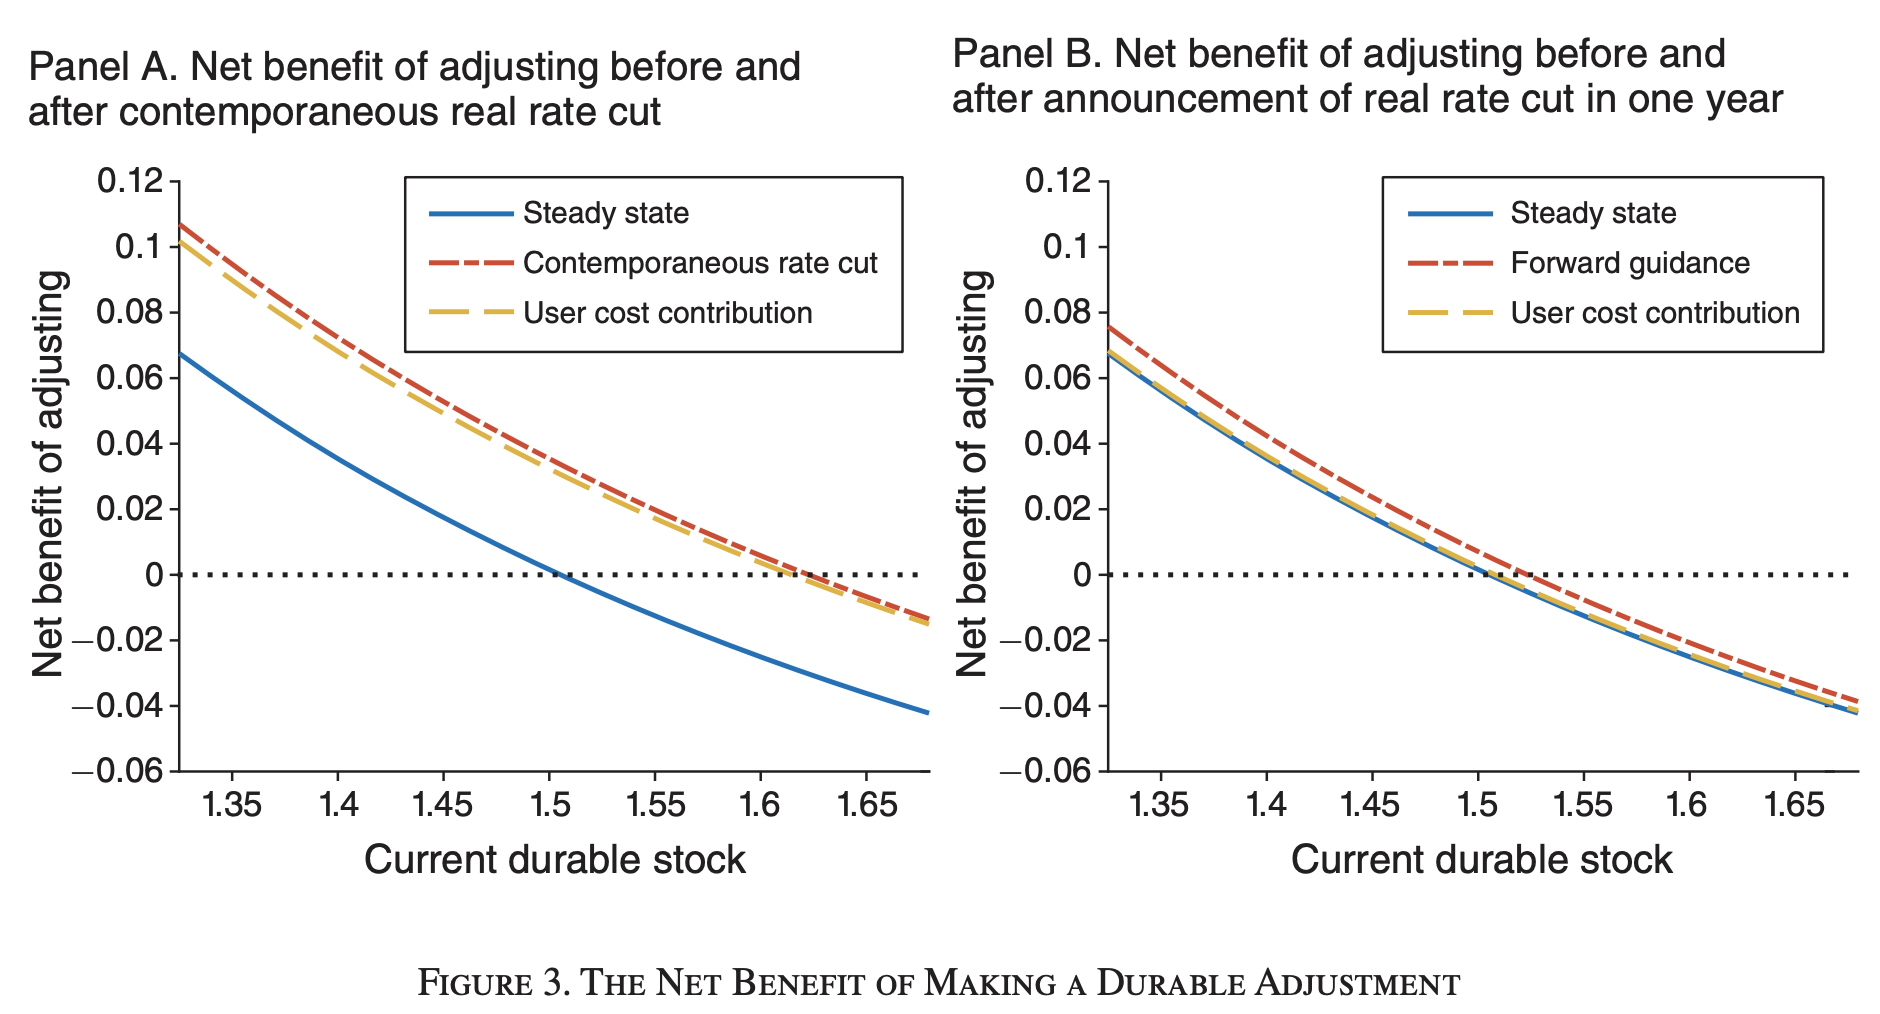
\includegraphics[scale=0.3]{figures/MWFGFIG3.png}	
    \end{center}
\end{frame}

\begin{frame}
    \frametitle{Intensive Margin}
\begin{align*}
		\E_t\int_0^{\tau} &e^{-(\rho+\delta(1-\chi)) s} u_d(c_{t+s},e^{-\delta(1-\chi) s}d)ds \\
		&=   \E_t e^{-\rho \tau}V_{x,t+\tau}^{adj}\left[r^d_{t,t+\tau}  + e^{-\delta(1-\chi) \tau}p_{t+\tau} f\right] \\
		& \qquad + \E_t\int_0^{\tau}e^{-\rho s}\Psi_{t+s}\left[r^d_{t,t+s} + (1-\lambda(1-f))e^{-\delta(1-\chi)s}p_{t+s}\right]ds \\
	\end{align*}
\begin{itemize}
	\item Intuition: survival probability decreasing in time.
\end{itemize}
\end{frame}

\begin{frame}
    \frametitle{Long-term financing}
\begin{itemize}
	\item FOC for extensive margin the same when durable financed with long-term debt.
	\item Intuition: adjust now vs a little bit later, so expected change in financing cost matters for adjustment.
\end{itemize}
\end{frame}

\begin{frame}
    \frametitle{Questions}
	\begin{itemize}
		\item Convincing?
		\item What role does the micro evidence play?
	\end{itemize}
\end{frame}

%%%%%%%%%%%%%%%%%%%%%%%%%%%%%%%%%%%%%%%%%%%%%%%%%%
\section{Beraja and Zorzi (2024)}
%%%%%%%%%%%%%%%%%%%%%%%%%%%%%%%%%%%%%%%%%%%%%%%%%%

\begin{frame}
    \frametitle{Question}
	\begin{itemize}
		\item How large a stimulus to close the output gap?
		\item Want to think about durables since important in determining MPCs as well as size and state-dependence.
		\item Why a model?
		% \item Involves both state dependence and time dependence.
		% \item Intertemporal dimension?
		% \item What disciplines size dependence?
	\end{itemize}
\end{frame}

% \begin{frame}
%     \frametitle{Why a Model?}
% 	% \begin{itemize}
% 	% 	\item Contradicting evidence in the empirical literature. (but lotteries should help?)
%     % 	\item Separate state dependence and size dependence? E.g., larger stimulus in deeper recession.
%     % 	\item Existing models focus on nondurables.
%     % 	\item Is this a question about state or size dependence?
% 	% \end{itemize}
% \end{frame}

\begin{frame}
    \frametitle{Model}
	\begin{itemize}
		\item Value function:
		\begin{align*}
            V_t(x,\epsilon) = \max\{V_t^{adj}(x) - \epsilon,V_t^{noadj}(x)\}
        \end{align*}
        where $x=(d,m,y)$.
        \item Adjustment utility:
        \begin{align*}
            V_t^{adj}(x) &= \max_{c,d',a'} u(x,d') + \beta \int V_{t+1}(d',m',y',\epsilon')d\mathcal{E}(\epsilon) \Gamma(dy',y) \\
            \text{s.t.} \; &\theta d' + c + m' = \mathcal{Y}(x,T_t) + ((1-\delta) - (1-\theta))d \\
            &m'\ge 0
        \end{align*}
        \item No adjustment utility:
        \begin{align*}
            V_t^{noadj}(x) &= \max_{c,a'} u(x,d') + \beta \int V_{t+1}(d',m',y',\epsilon')d\mathcal{E}(\epsilon) \Gamma(dy',y) \\
            \text{s.t.} \; &  c + m' = \mathcal{Y}(x,T_t) -\iota \delta d - (1-\theta)(d-d') \\
            &d' = (1 - (1-\iota)\delta) d \\
            &m'\ge 0 
        \end{align*}
	\end{itemize}
\end{frame}

\begin{frame}
    \frametitle{Importance of the Hazard}
    \begin{center}
    	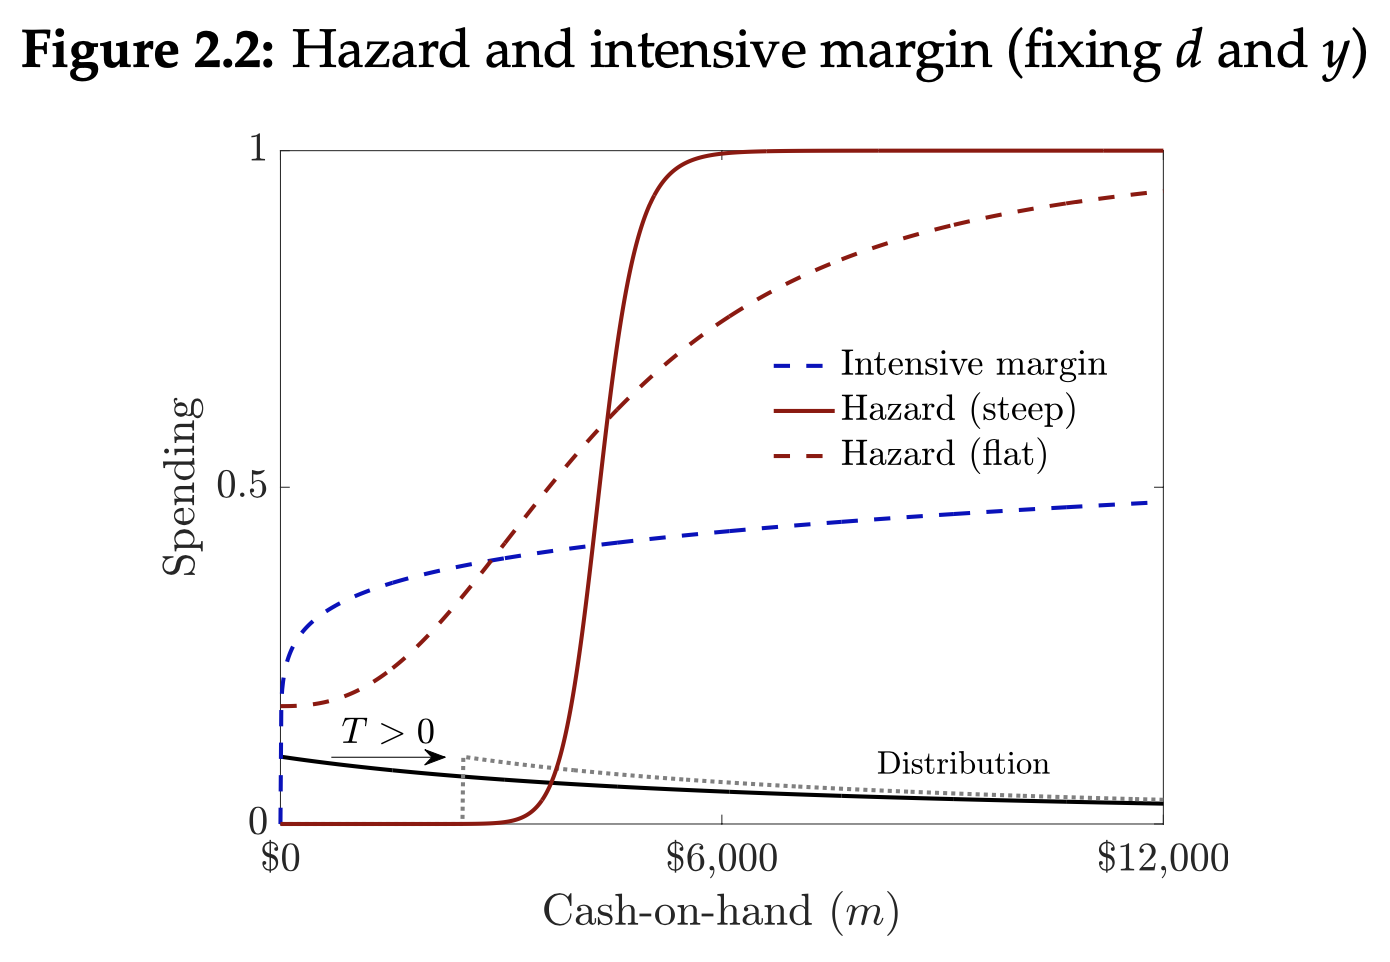
\includegraphics[scale=0.4]{figures/BZFIG22.png}	
    \end{center}
\end{frame}

\begin{frame}
    \frametitle{Why is this a good model?}
	\begin{itemize}
		\item How convincing did you find section 3?
	\end{itemize}
\end{frame}

% \begin{frame}
%     \frametitle{Thoughts}
% 	\begin{itemize}
% 		\item v Calvo plus: different way of targeting. is it apples to apples?
% 		\item must be that calvo plus hazard is steeper so more interest rate senstitive?
% 		\item seems plausible since the smooth hazard means we take more HH away from the edges of the adjustment bands.
% 	\end{itemize}
% \end{frame}



\begin{frame}
    \frametitle{Calibrating the Hazard (1)}
    \begin{center}
    	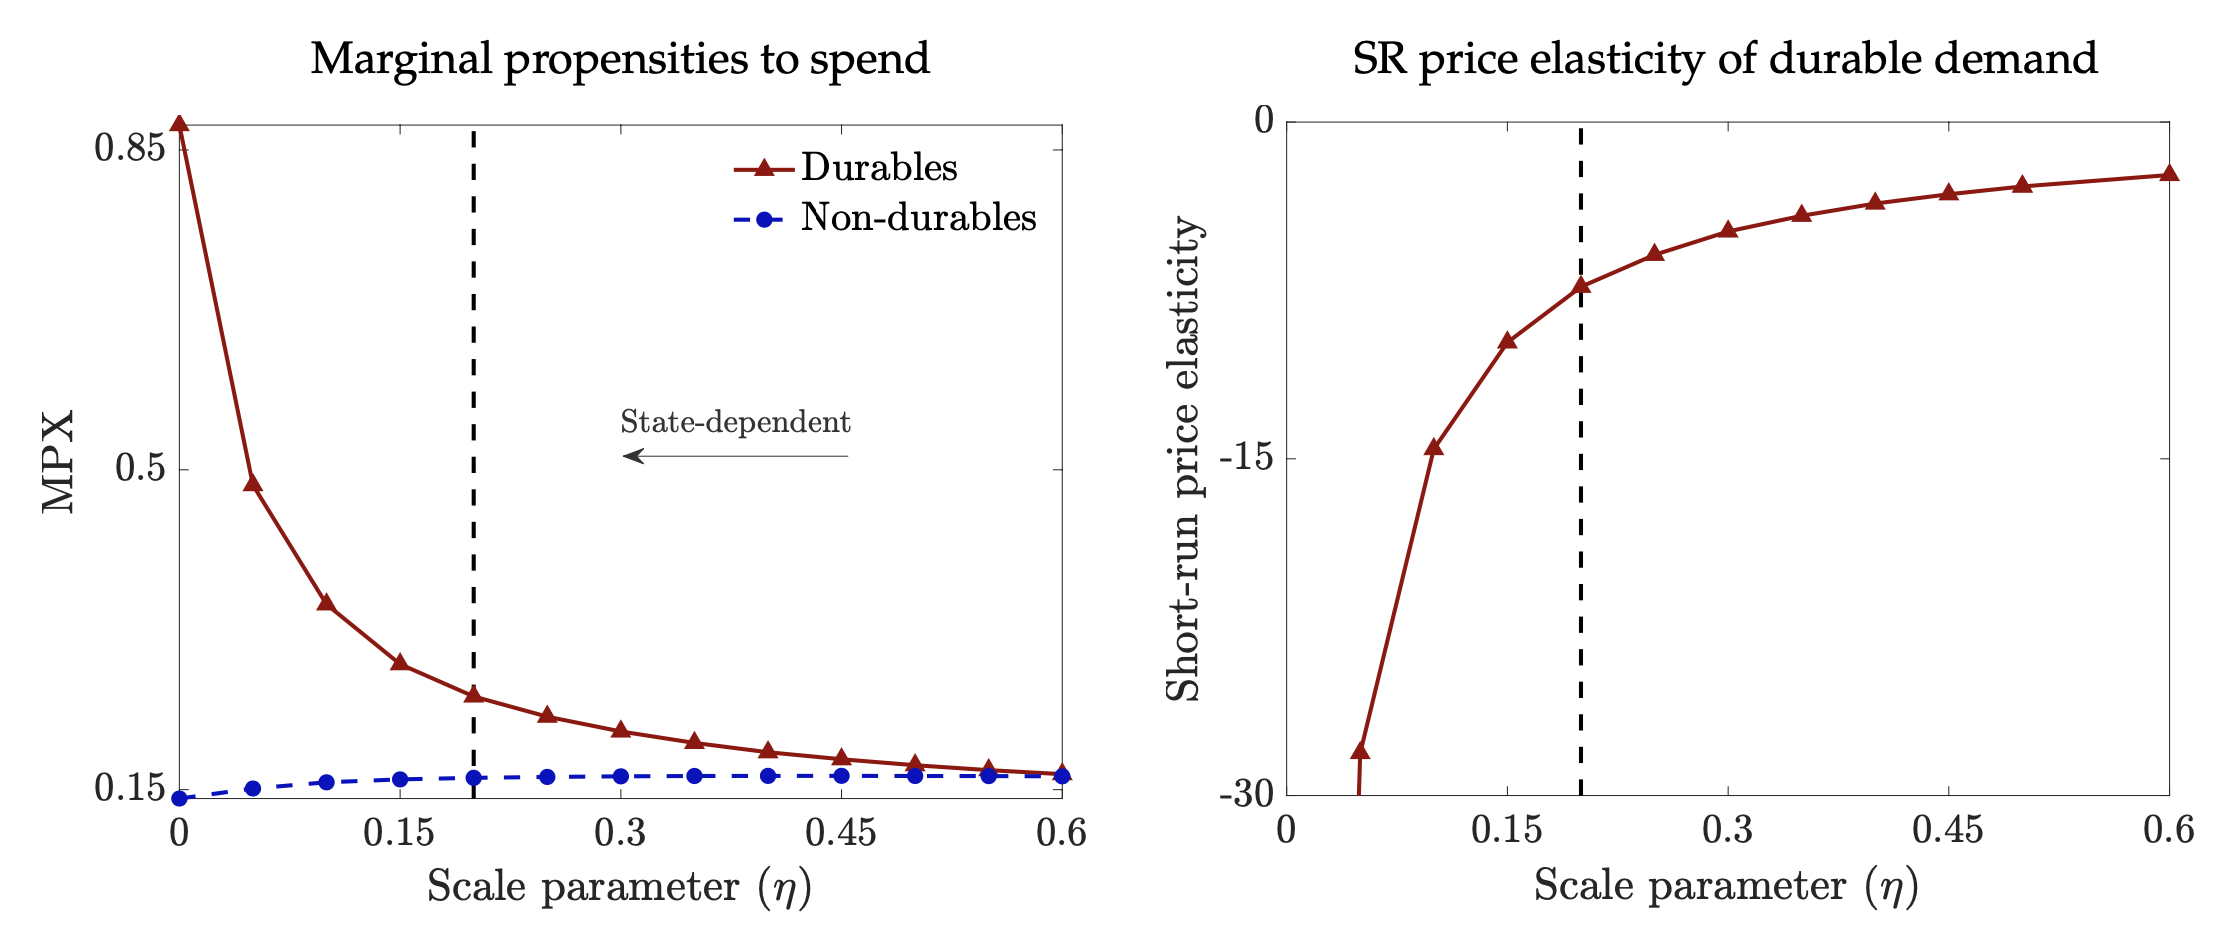
\includegraphics[scale=0.3]{figures/BZFIG31.png}	
    \end{center}
\end{frame}

\begin{frame}
    \frametitle{Calibrating the Hazard (2)}
    \begin{center}
    	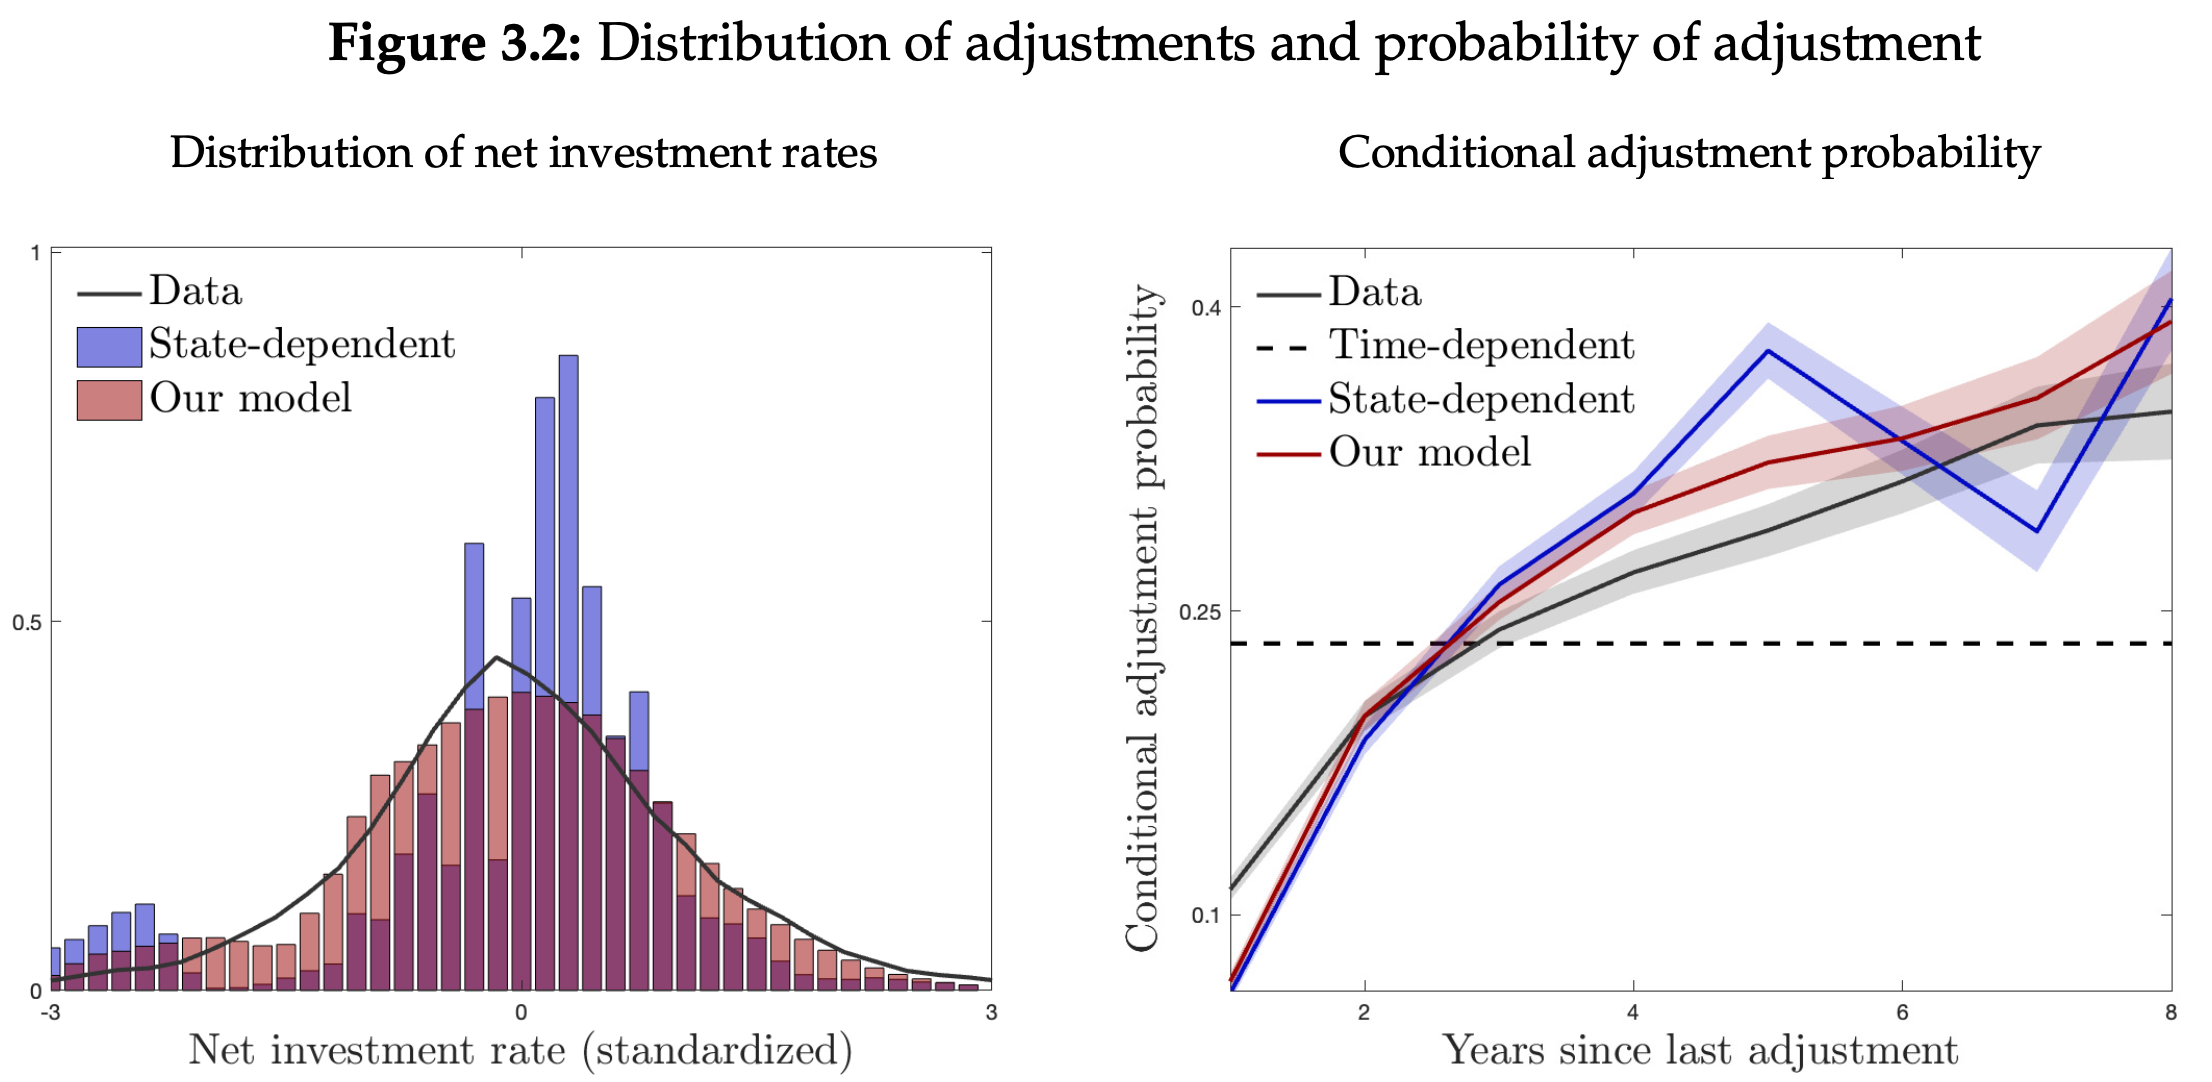
\includegraphics[scale=0.3]{figures/BZFIG32.png}	
    \end{center}
\end{frame}

\begin{frame}
    \frametitle{MPX in the Model vs Alternatives}
    \begin{center}
    	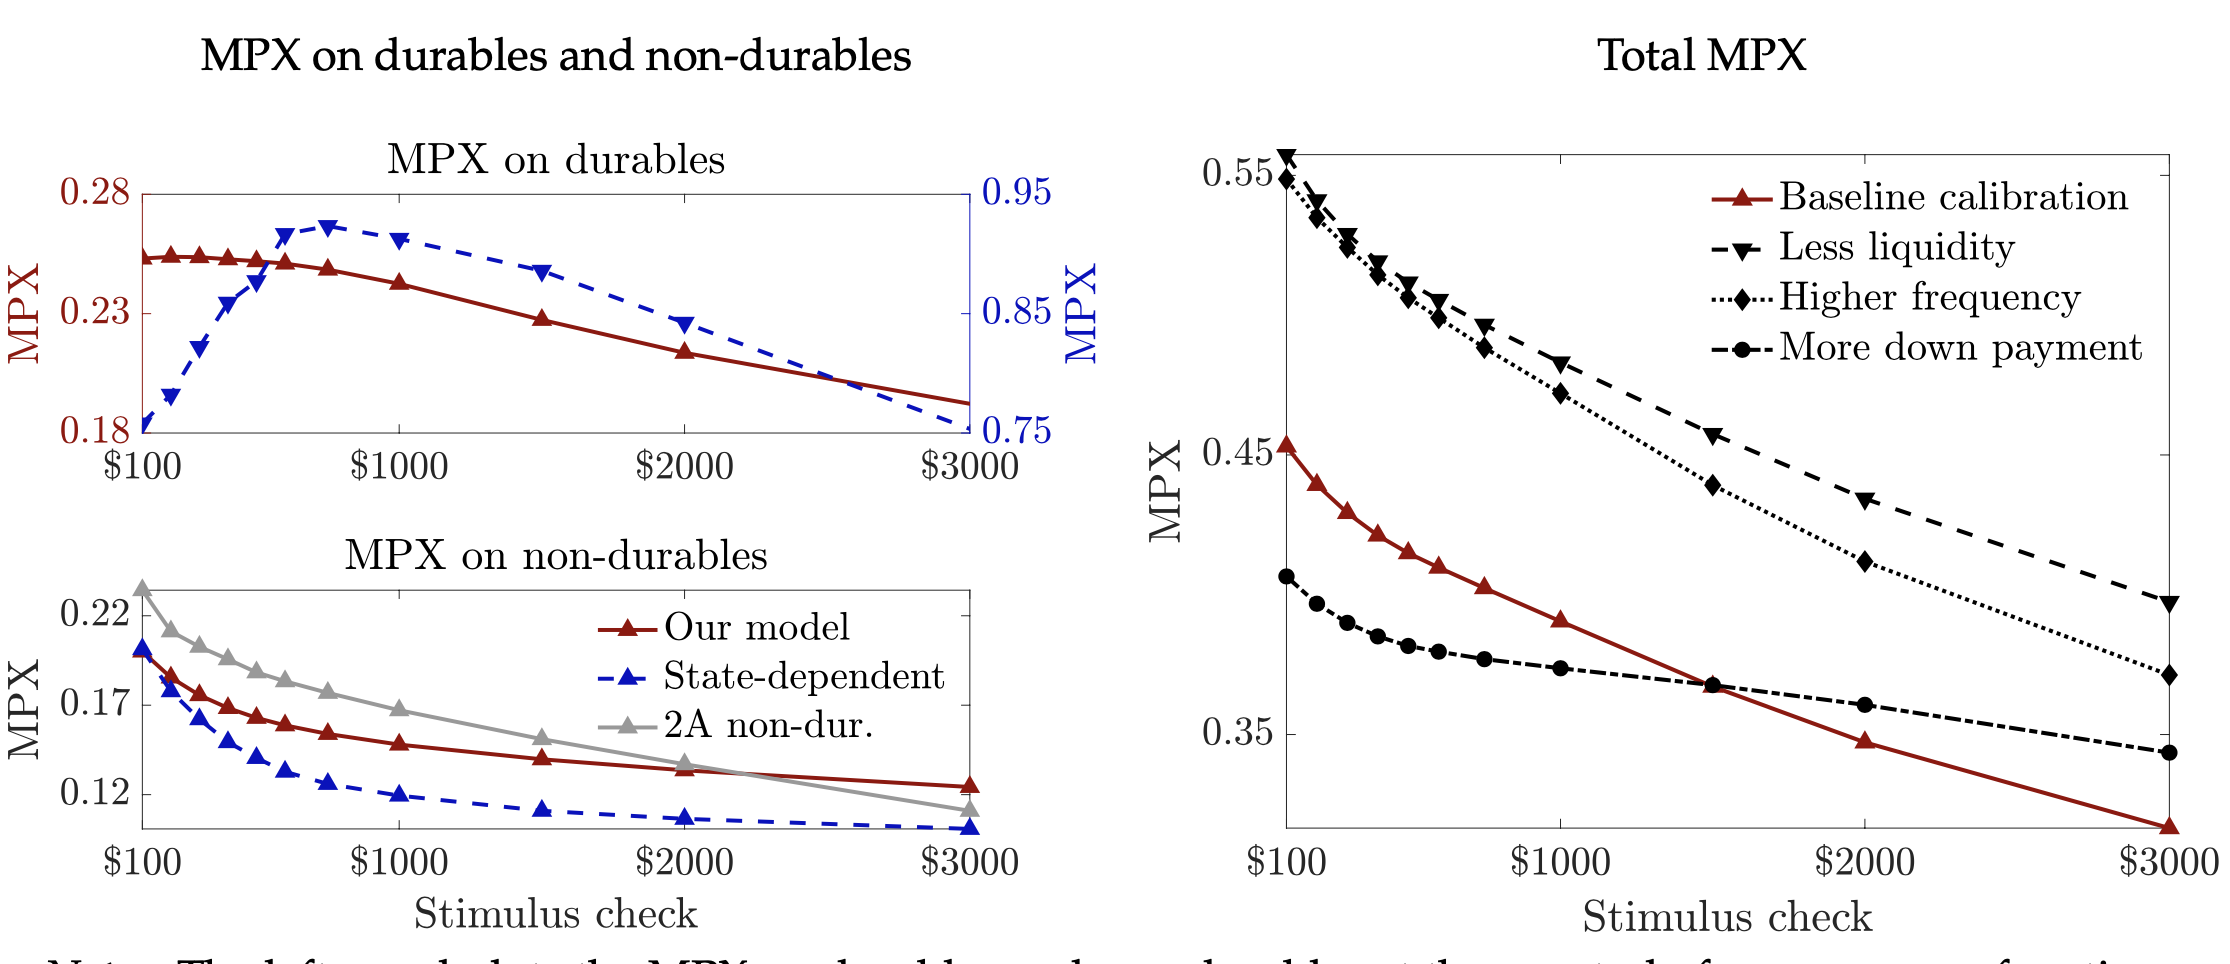
\includegraphics[scale=0.3]{figures/BZFIG41.png}	
    \end{center}
\end{frame}

\begin{frame}
    \frametitle{GE MPCs}
    \begin{center}
    	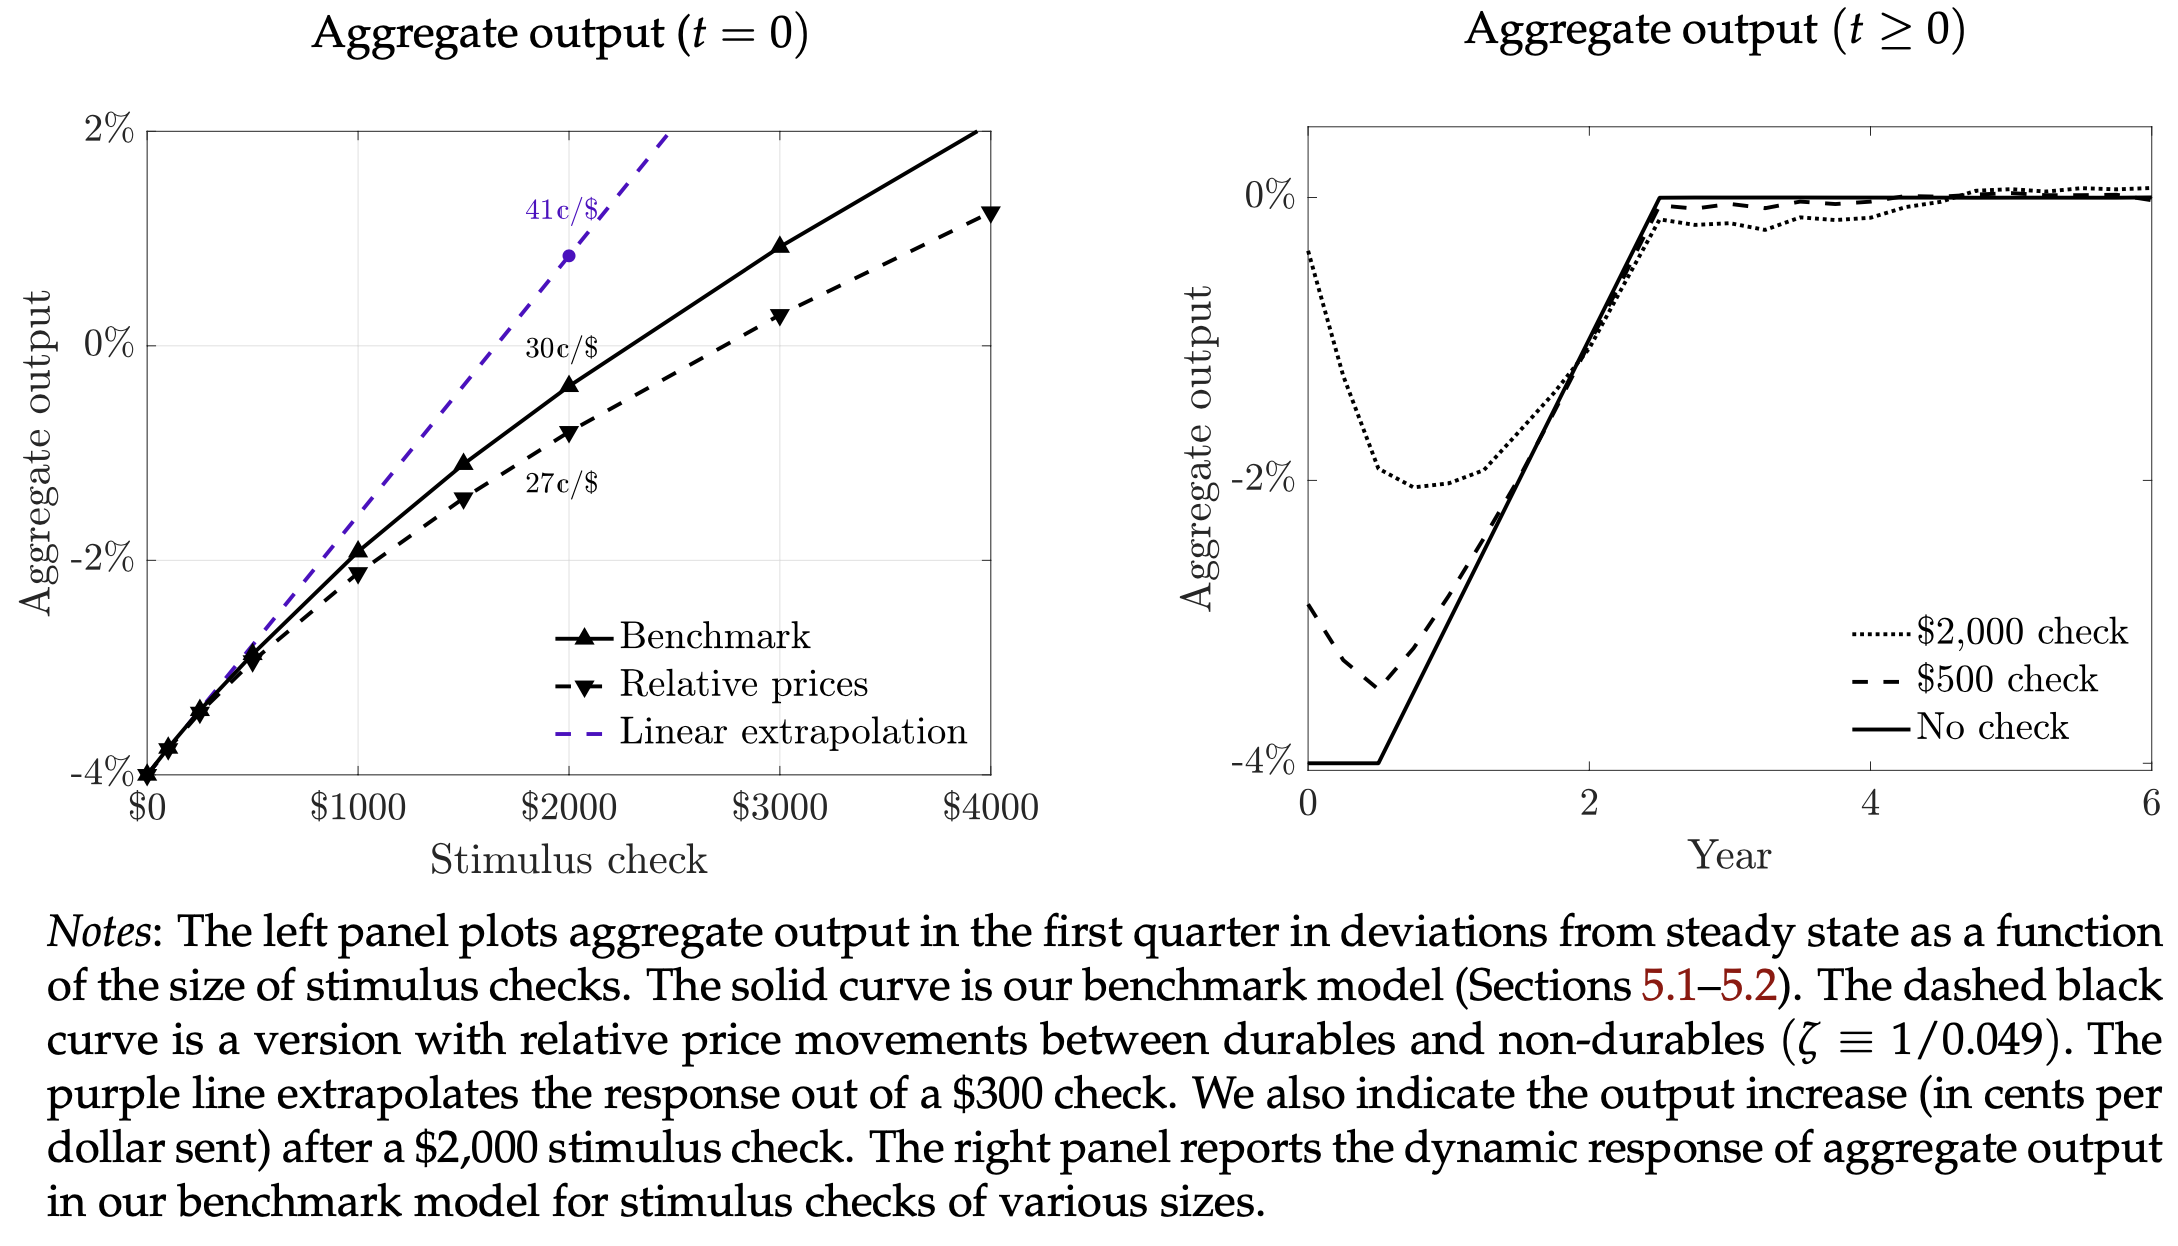
\includegraphics[scale=0.3]{figures/BZFIG51.png}	
    \end{center}
\end{frame}



\begin{frame}
    \frametitle{What did you think?}
	% \begin{itemize}
	% 	\item Better empirical description.
	% 	\item Controls size dependence (sufficient statistic?)
	% 	\item Targets: small shock MPX, short-run price elasticity, durable adjustment distribution
	% \end{itemize}
\end{frame}

\end{document}